\documentclass[11pt,DIV=13,BCOR=5mm,a4paper,headinclude]{scrbook}
%\usepackage[ngerman]{babel}
\usepackage[english]{babel}
\usepackage[latin1]{inputenc}
\usepackage[T1]{fontenc}
\usepackage{lmodern}
\usepackage{upgreek}
%\usepackage{graphicx}
\usepackage[figuresright]{rotating}	% l�dt auch graphicx
\usepackage{caption}
\usepackage{xcolor}
\usepackage{amsmath}
\usepackage{amssymb}
\usepackage[version=3]{mhchem} % Formula subscripts using \ce{}
\usepackage{setspace}
\usepackage{titletoc}
\usepackage{scrpage2}
\usepackage{textcomp}
\usepackage{ragged2e}
\usepackage{booktabs}
\usepackage{threeparttable}
\usepackage[sf,SF]{subfigure}
\renewcommand\thesubfigure{\,(\alph{subfigure})}
\usepackage{rotating}
\usepackage{enumitem}
\usepackage{multirow}
\usepackage{color}
\usepackage{ulem}
\usepackage{etoolbox}
\usepackage{bibentry}
\usepackage{placeins}
\usepackage{cite}
%\nobibliography*

\clubpenalty = 10000
\widowpenalty = 10000

\linespread{1.25}
\KOMAoptions{DIV=last}

%Links im Inhaltsverzeichnis
\usepackage{hyperref}
\hypersetup{colorlinks,citecolor=black,filecolor=black,linkcolor=black,urlcolor=black}

%Eigene Befehle
\newcommand*{\mystrut}{\rule[-.2\baselineskip]{0pt}{-.2\baselineskip}}
\renewcommand*{\dictumwidth}{0.618\textwidth}
\renewcommand*{\partpagestyle}{empty}
\setlength{\parskip}{0pt}

%Eigene Mathebefehle
\def\mathbi#1{\textbf{\em #1}}
\renewcommand{\vec}[1]{\mathbi{#1}}
\renewcommand{\i}{{\mathrm{i}}}
\addtokomafont{disposition}{\boldmath}

%�berschriften
\addtokomafont{part}{\huge}
\addtokomafont{chapter}{\LARGE}
\addtokomafont{section}{\Large}
\addtokomafont{subsection}{\large}
\addtokomafont{subsubsection}{\large\sffamily\textit}

%Captions anpassen
\setcapindent{1em}
\setkomafont{captionlabel}{\sffamily\bfseries}
\setkomafont{caption}{\sffamily}
%\addtokomafont{caption}{\small\sffamily}
\KOMAoption{captions}{outerbeside}

%Fu�noten
\usepackage[bottom,hang]{footmisc}
\setlength{\skip\footins}{\baselineskip}
\setlength{\footnotesep}{0.75\baselineskip}
\deffootnote[1.0em]{0.0em}{1.0em}{\textsuperscript{\thefootnotemark~}}

%Listen anpassen
\setlist[enumerate]{rightmargin=\leftmargin,noitemsep,label=(\arabic*)}

%Boxen anpassen
\setlength{\fboxsep}{0pt}
\setlength{\fboxrule}{1pt}

%Kopfzeile
\pagestyle{scrheadings}
\clearscrheadfoot
\renewcommand*{\partmarkformat}{}
\automark[section]{chapter}
\lehead[]{\leftmark}
\rohead[]{\rightmark}
\lefoot[\pagemark]{\pagemark}
\rofoot[\pagemark]{\pagemark}

%Appendix
\newcommand*{\appendixmore}{
\renewcommand{\thesection}{\Alph{section}}
\numberwithin{equation}{section}
\numberwithin{table}{section}
}

%Literaturverzeichnis
%\addto\captionsngerman{
\addto\captionsenglish{
\renewcommand{\bibname}{}%
\renewcommand{\refname}{}}

%Worttrennung
\hyphenation{Dis-per-sion}
\hyphenation{Dis-per-sions-kor-rek-tu-ren}
\hyphenation{Dif-fu-sion}
\hyphenation{Kern-elek-tron}
\hyphenation{in-te-res-san-ten}
\hyphenation{dis-so-zi-iert}
\hyphenation{Quan-ten-effekt}
\hyphenation{Syn-the-se}
\hyphenation{Nor-mal-mo-den-a-na-ly-sen}
\hyphenation{Nor-mal-mo-den-a-na-ly-se}
\hyphenation{Zeit-ska-la}
\hyphenation{Ge-ne-ra-lized}
\hyphenation{Grund-zu-stands-po-ten-tial-fl�-che}
\hyphenation{Stick-stoff-a-to-me}
\hyphenation{Sub-strat-ober-fl�-che}
\hyphenation{Be-deckungs-grad}
\hyphenation{Be-deckungs-gra-de}

%%%%%%%%%%%%%%%%%%%%%%%%%%%%%%%%%%%%%%%%%%%%%%%%%%%%%%%%%%%%%%%%%%%%%%%%%%%%%%%%%%%%%%%%%%%%%%%%%%%%%%%%%%%%%%%%%%%%%%%%%%%%%%%%%%%%%%%%%%%%%%%%%%%%%%%%%%%%%%%%%%%%%%%%%%%%%%%%%%%%%%%%%%%%%%%%%%%%%%%%%%%%%%%%%%%%%%%%%%%%%%%%%%%%%%%%%%%%%%%%%%%%%%%%%%%%%%%%%%%%%%%
%%%%%%%%%%%%%%%%%%%%%%%%%%%%%%%%%%%%%%%%%%%%%%%%%%%%%%%%%%%%%%%%%%%%%%%%%%%%%%%%%%%%%%%%%%%%%%%%%%%%%%%%%%%%%%%%%%%%%%%%%%%%%%%%%%%%%%%%%%%%%%%%%%%%%%%%%%%%%%%%%%%%%%%%%%%%%%%%%%%%%%%%%%%%%%%%%%%%%%%%%%%%%%%%%%%%%%%%%%%%%%%%%%%%%%%%%%%%%%%%%%%%%%%%%%%%%%%%%%%%%%%
%%%%%%%%%%%%%%%%%%%%%%%%%%%%%%%%%%%%%%%%%%%%%%%%%%%%%%%%%%%%%%%%%%%%%%%%%%%%%%%%%%%%%%%%%%%%%%%%%%%%%%%%%%%%%%%%%%%%%%%%%%%%%%%%%%%%%%%%%%%%%%%%%%%%%%%%%%%%%%%%%%%%%%%%%%%%%%%%%%%%%%%%%%%%%%%%%%%%%%%%%%%%%%%%%%%%%%%%%%%%%%%%%%%%%%%%%%%%%%%%%%%%%%%%%%%%%%%%%%%%%%%

\begin{document}

%Titelseite
\title{WORKING TITLE:\\
  Quanteneffekte, Wasser auf Metalloxidoberfl�chen\vspace{2\baselineskip}}
\subtitle{\normalfont\sffamily Dissertation zur Erlangung des akademischen Grades\\
  {\frq}doctor rerum naturalium{\flq} (Dr. rer. nat.)\\
  in der Wissenschaftsdisziplin Theoretische Chemie}
\author{\sffamily\large vorgelegt von\\
  \sffamily\Large\bfseries Sophia L. Heiden}
\publishers{\sffamily\large an der\\
  Mathematisch-Naturwissenschaftlichen Fakult�t\\
  der Universit�t Potsdam\\ \vspace{1.5\baselineskip}
  
\includegraphics[width=0.1\textwidth]{figures/UP-Logo_Matjpg.jpg}\\ \vspace{\baselineskip}
  Potsdam, xx 2018}
\date{}

\uppertitleback{\normalfont
This work has been done between January 2015 and xx 2018 in the workgroup of Prof. Dr. Peter Saalfrank at the Institute of Chemistry at the University of Potsdam.
}
\lowertitleback{Potsdam, xx 2018\\
\begin{tabular}{ll}
Erstgutachter: &Prof. Dr. Peter Saalfrank (Uni Potsdam) \\
Zweitgutachter:&Prof. Dr. Beate Paulus (FU Berlin)\\
Drittgutachter:&Prof. Dr. xy \\
\end{tabular}
 }

%\dedication{F�r meinen Vater.}

\maketitle

%%%%%%%%%%%%%%%%%%%%%%%%%%%%%%%%%%%%%%%%%%%%%%%%%%%%%%%%%%%%%%%%%%%%%%%%%%%%%%%%%%%%%%%%%%%%%%%%%%%%%%%%%%%%%%%%%%%%%%%%%%%%%%%%%%%%%%%%%%%%%%%%%%%%%%%%%%%%%%%%%%%%%%%%%%%%%%%%%%%%%%%%%%%%%%%%%%%%%%%%%%%%%%%%%%%%%%%%%%%%%%%%%%%%%%%%%%%%%%%%%%%%%%%%%%%%%%%%%%%%%%%
%%%%%%%%%%%%%%%%%%%%%%%%%%%%%%%%%%%%%%%%%%%%%%%%%%%%%%%%%%%%%%%%%%%%%%%%%%%%%%%%%%%%%%%%%%%%%%%%%%%%%%%%%%%%%%%%%%%%%%%%%%%%%%%%%%%%%%%%%%%%%%%%%%%%%%%%%%%%%%%%%%%%%%%%%%%%%%%%%%%%%%%%%%%%%%%%%%%%%%%%%%%%%%%%%%%%%%%%%%%%%%%%%%%%%%%%%%%%%%%%%%%%%%%%%%%%%%%%%%%%%%%
%%%%%%%%%%%%%%%%%%%%%%%%%%%%%%%%%%%%%%%%%%%%%%%%%%%%%%%%%%%%%%%%%%%%%%%%%%%%%%%%%%%%%%%%%%%%%%%%%%%%%%%%%%%%%%%%%%%%%%%%%%%%%%%%%%%%%%%%%%%%%%%%%%%%%%%%%%%%%%%%%%%%%%%%%%%%%%%%%%%%%%%%%%%%%%%%%%%%%%%%%%%%%%%%%%%%%%%%%%%%%%%%%%%%%%%%%%%%%%%%%%%%%%%%%%%%%%%%%%%%%%%

\addchap{Preamble}
The importance of surface science in our industrialized world is overwhelming, because most processes in industry need (heterogeneous) catalysts, because these do not have to be separated from the reactands and the product after the process, which is mostly a costly step in the production of chemicals. It is therefore desirable to understand heterogeneous catalytic processes by learning more about the processes that take place on the surface of materials. Metal oxide materials are frequently used in catalysts as well as catalyst support materials, so that understanding their properties in contact with chemicals, in this work water, is crucial.
\\

Aluminum is used in rocket fuels as a reduction agent so that during launch alumina particles are ejected in the atmosphere during the start (see also lit.dat!). For a space shuttle the start can produce around $760,000\,$kg of alumina particles. It can be measured that approximately one third of these particles can be deposited in the stratosphere (in an altitude between $15$ and $50\,$km above the surface of the earth) and there it can react with the water and other molecules in the stratosphere where these particles are accumulated after the launch of a shuttle.
\\

Also in geochemical sciences Al$_2$O$_3$ is a subject of a variety of studies since aluminum is the third most common element in the crust with $6.3\%$ ({\color{red} \begin{verbatim} http://www.uniterra.de/rutherford/tab_hauf.htm\end{verbatim}}
{\textit{Riedel\cite{Riedel}: Alumina is the most abundant metal in the crust and the third most element therein. Component of  feldspar, Glimmer and clay minerals (with silicates), more seldomly as corundum and "Schmirgel". Some of them are precious stones ruby, saphir}\\
Dtv-Atlas\cite{dtv-Atlas}: third most abundant element, $8.1\%$ of the earth crust and with that the far most abundant metal}
) and it also can be seen as a model systems for more complex alumosilicates. Oxide rocks are omnipresent in the crust of the earth and henceforth in most geochemical processes since the times the earth's atmosphere became oxidizing with rise of photosynthetic life forms/(bacteria?) a few million years ago. Before under reductive conditions sulfidic rocks were dominant but when photosynthesis became more common with the rise of more advanced life forms, the oxygen content of the atmosphere grew.


%%%%%%%%%%%%%%%%%%%%%%%%%%%%%%%%%%%%%%%%%%%%%%%%%%%%%%%%%%%%%%%%%%%%%%%%%%%%%%%%%%%%%%%%%%%%%%%%%%%%%%%%%%%%%%%%%%%%%%%%%%%%%%%%%%%%%%%%%%%%%%%%%%%%%%%%%%%%%%%%%%%%%%%%%%%%%%%%%%%%%%%%%%%%%%%%%%%%%%%%%%%%%%%%%%%%%%%%%%%%%%%%%%%%%%%%%%%%%%%%%%%%%%%%%%%%%%%%%%%%%%%
%%%%%%%%%%%%%%%%%%%%%%%%%%%%%%%%%%%%%%%%%%%%%%%%%%%%%%%%%%%%%%%%%%%%%%%%%%%%%%%%%%%%%%%%%%%%%%%%%%%%%%%%%%%%%%%%%%%%%%%%%%%%%%%%%%%%%%%%%%%%%%%%%%%%%%%%%%%%%%%%%%%%%%%%%%%%%%%%%%%%%%%%%%%%%%%%%%%%%%%%%%%%%%%%%%%%%%%%%%%%%%%%%%%%%%%%%%%%%%%%%%%%%%%%%%%%%%%%%%%%%%%
%%%%%%%%%%%%%%%%%%%%%%%%%%%%%%%%%%%%%%%%%%%%%%%%%%%%%%%%%%%%%%%%%%%%%%%%%%%%%%%%%%%%%%%%%%%%%%%%%%%%%%%%%%%%%%%%%%%%%%%%%%%%%%%%%%%%%%%%%%%%%%%%%%%%%%%%%%%%%%%%%%%%%%%%%%%%%%%%%%%%%%%%%%%%%%%%%%%%%%%%%%%%%%%%%%%%%%%%%%%%%%%%%%%%%%%%%%%%%%%%%%%%%%%%%%%%%%%%%%%%%%%

%Inhaltsverzeichnis
\renewcommand{\contentsname}{Contents}
\clearpage
%\pagestyle{empty}
%\renewcommand*{\chapterpagestyle}{empty}
\tableofcontents
\clearpage
%\pagestyle{useheadings}
%\renewcommand*{\chapterpagestyle}{plain}

%%%%%%%%%%%%%%%%%%%%%%%%%%%%%%%
%Abk�rzungsverzeichnis?
%Abbildungsverzeichnis?
%Tabellenverzeichnis?
%%%%%%%%%%%%%%%%%%%%%%%%%%%%%%%
\chapter{Theory und Methodology}
In this chapter the basics of the applied theoretical methods shall be explained.
\section{DFT}
basic idea of DFT, only 3 dimensional system instead of 3N-dimensional with N being the number of electrons, Kohn-Sham DFT use orbitals again, methods amd algorithms known from wave function based methods can be applied, functionals difference pure density functionals and hybrid, some exact exchange from Hartree Fock is mixed into the potential, functionals like B3LYP, HSE06. Dispersion corrections that account for van-der-Waals interactions, and are important for the adsorbate-surface interaction and the adsorbate-adsorbate interaction.

A test system with non-interacting electrons that reflects the systems electron density, is set and calculated.

Hohenberg-Kohn theorem connect the Hamiltonian of a many-particle system to its ground-state density $n(\vec{r})$. If $\Psi(\vec{r}^N)$ is an N-electron wavefunction, then the  electron density can be given as
\begin{equation}
 n(\vec{r})=N\int ... \int \Psi^\ast(\vec{r},\vec{r}_2,\vec{r}_3...,\vec{r}_N)\Psi(\vec{r},\vec{r}_2,\vec{r}_3...,\vec{r}_N) d \vec{r}_2...d \vec{r}_N 
\end{equation}
with Hohenberg-Kohn Theorem I the total energy $E[n]$ can be determined as:
\begin{equation}
 E[n]=T[n] + V_{ext}[n] + V_{ee}[n]=\int n(\vec{r})v_{ext}(\vec{r})d\vec{r} + T[n]+E_H[n]+E_{xc}[n]
\end{equation}
with the kinetic energy $T[n]$, the potential energy $V[n]$ for electron electron interaction $ee$ and  external potential $ext$, the Hartree energy $E_H[n]$, corresponding to the classical Coulomb interaction and the exchange correlation energy $E_{xc}[n]$ for the non-classical exchange correlation interactions.
\\
A problem is, that the explicit form of the interacting kinetic energy $T[n]$ and the exchange correlation functional $E_{xc}[n]$ are unknown.



\section{Periodic Boundary Conditions}
plane wave basis, no atom centered basis functions, periodic boundary conditions, electron density has to be the same in each repeating unit, Miller Indices for nomenclature of surface sites/faces (3 and 4 numbers) (hkl, hk-(h+k)l), how to understand these numbers, hexagonal cells, lattice types, differences between these types, Bravais lattice, Brillouin zone, $\vec{k}$-points, irreducible $\vec{k}$-points necessary for describing the system, direct and reciproce room, how to convert between these two with the lattice vectors
\\
Surface simulation, 2-D system reproduced as 3-D structure since vasp is bulk code there have to be 3 dimensions, so one has to define a vacuum gap between two slabs along the z-axis (perpendicular to the surface) to prevent unit cells from influencing each other and therefore lead to unphysical behaviour. Some programs (here used crystal and cp2k(?)) deliver opportunity to calculate only 2D system, repeating the slab only in x/y, a/b, respectively.
\\
The systems are modelled as periodic solid, this can be described by a unit cell, that is translated along every spatial direction.
The lattice can be described by the lattice vector $\vec{B}$. $\vec{a}_i$ are basis vectors of the lattice and $n_i$ integers:
\begin{equation}
 \vec{B}=n_1\vec{a}_1+n_2\vec{a}_2+n_3\vec{a}_3
\end{equation}
Analogue to that, also a reciproce space exists ($\vec{k}$-space) with a set of vectors $\vec{G}$:
\begin{equation}
 \vec{G}=h\vec{b}_1+k\vec{b}_2+l\vec{b}_3
\end{equation}
that span the lattice space. For the reciproce space we have:
\begin{equation}
 e^{i\vec{G}\vec{B}}=1.
\end{equation}
The unit cell withing the reciprocal space is called Wigner-Seitz cell and is also referred to as first Brillouin zone, whose center is the $\Gamma$-point ($h=k=l=0$). Between the vectors of the direct and the reciprocal space there are fixed relations and the are perpendicular to each other:
\begin{equation}
 \vec{a}_i\cdot\vec{b}_j=2\pi\delta_{ij}.
\end{equation}

To describe periodic systems with quantum mechanical methods, one has to introduce periodic boundary conditions. These assume that the effective potential $v_{eff}$ has to be the same in all cells that are given by $\vec{B}$:
\begin{equation}
 v_{eff}(\vec{r})= v_{eff}(\vec{r}+\vec{B}).
\end{equation}


\section{Atom Centered Basis and Peculiarities}
Problem of plane waves for necessity of atom centered bases; Whenver there are atom centered basid sets the orbitals can overlap and due to this electrons are considered multiple times. This is called Basis Set Superposition Error (BSSE). One can apply Counterpoise corrections to get rid of this source of error. This is done here by calculating ghosted calculations with the system as a whole, the adsorbate alone, and the adsorbate with surface from ghost atoms. Then one applies a substractive scheme to cancel out the effect of the orbital overlap. On the other hand one can use a huge basis set, that doesn't have this problem, which comes with a higher computational demand.


\section{{\textit Ab-initio} Molecular Dynamics}
Microcanonical and Canonical ensemble, also called NVT and NVE. Difference between the two, N number of (?), V volume of the cell, T temperature and E energy; are kept constant. theory behind, calcuation of time propagation with Verlet algorithm, time steps chosen so that we don't miss the fastest processes, forces acting on atoms, Nos\'{e} Hoover thermostat.
\\
Solve Newton's equations of motion, in principle $F=m\cdot a$ for force acting on each atom, classical ansatz.
\begin{equation}
 -\frac{\partial V(\vec{R})}{\partial \vec{R}(t)}=M_A\frac{d^2 \vec{R}_A(t)}{dt^2}
\end{equation}

\section{Frequencies and Intensities}
Normal Mode Analysis, diagonalization of the Hessian, eigenvalues are frequencies squared. While this is a good approximation for the high energy vibration, for example OD stretch vibrations, it becomes worse for lattice vibrations, which are way more delocalized.
A characteritic of stationary points on the potential energy surface is, that the derivation with respect to all coordinates equals 0. For these points (minima and saddle points of first order) the Hessian matrix and their eigenvalues are of interest. The elements of this Hessian are the derivation of the potential with respect to coordinates:
\begin{equation}
 H_{ij}=\left( \frac{\partial^2 V}{\partial Q_i \partial Q_j} \right)_{|Q_i=Q_j=0}=\left(\frac{1}{\sqrt{m_i m_j}} \frac{\partial^2 V}{\partial R_i \partial R_j} \right)
\end{equation}
Here, $Q_i$ are mass weighted coordinates $Q_i=\sqrt{m_i}R_i$, with the mass $m_i$ and the displacement from the equilibrium position $R_i$.
Then the matrix problem for the Hessian ${\color{red} H}$ has to be solved:
\begin{equation}
 \stackrel{H}{=}\vec{A}_i=\lambda_i\vec{A}_i.
\end{equation}
with the vectors of the normal modes $A_i$ and $\lambda_i$ being the squares of vibrational freqencies $\omega_i$: 
\begin{equation}\label{eq:omegafromlambda}
 \omega_i=\sqrt{\lambda_i}.
\end{equation}
One has to distinguish two physically relevant cases: all eigenvalues are positive ($\lambda_i\geq 0 \forall i$) so the structure is a minimum on the PES. This could be the educt and product of a reaction. The second relevant case is if there is only one negative eigenvalue, that gives according to equation \ref{eq:omegafromlambda} one imaginary frequency, respectively. This is in a mathematical sense a saddlepoint of first order and can be interpreted as a transition state.
\\
dipole corrected NMA intensity can be calculated for IR spectra, not the same selection rules as for SFG but as a first approach should be feasible. Selection rules for SFG IR+Raman active, also the medium must not be version symmetric. {\color{red} put the selection rules into the experimental details section?}
\\
Tests with Born-effective charges: Intensities are also calculated via Born effective charges (BEC) where surface charges are determined and from that the intensities are obtained (dipole = charge*distance, $\mu^2\propto I$).
\\
Calculation of power spectra via velocity-velocity autocorrelation function from canonical MD trajectories. The vibrational density of states (VDOS) can be interpreted as the peaks of the spectrum. Through the motion of the atoms already some kind of quantum effects (not explicitly) are included.
\begin{equation}
 VDOS(\omega)=\sum_{i=1}^N\int_{-\infty}^{+\infty}<v_i(t)\cdot v_i(0)>e^{i\omega t}dt
\end{equation}

\section{Finding Transition States}
One of the most prominent theories describing the transition state and the rate constants is Eyring theory of transition states {\color{red} figure of reaction path?}. The most important approximations that are made are the following: all particles that reached the transition state will react towards the product. at the transition state geometry, the motion along the reaction coordinate can be separated from all other degrees of freedom and can be seen as a translation.
The equation for the rate constant is described by
\begin{equation}\label{eyring}
k(T)=\kappa\frac{k_BT}{h}e^{\Delta G^\ddagger(T)/(k_BT)},
\end{equation}
with the reaction rate constant $k$, Boltzmann's constant $K_B$, the temperature $T$, the difference of Gibb's free energy for the transition state and the educt $\Delta G^\ddagger$ and the transmission coefficient $\kappa$, that is a tunneling constant prefactor [tunneling corrections (seldomly applied in this work, not mention them here?)], give the reaction rate constant as a function of temperature and barrier height. For the latter one needs to find the energies of the transition state and the educt. The educt geometry can simply be obtained by geometry optimization as a minimum on the PES.
To find the transition state geometry and henceforth the energy we used Nudged Elastic Band calculations (NEB), with Climbing Image, Reaction path is approximated as a series of associated images, which are connected via spring forces. These spring forces prevent the images from optimizing into the local minimum next to the transition state. First a regular NEB, then afterwards climbing image was done which gives better convergence. In this calculation the energetically highest image is "optimized" towards higher energies in the contrary direction of the gradient.For the point found by this scheme we checked whether this is a transition state via frequency analysis, since a TST of first order has to have one imaginary mode, that vibrates alongside the reaction path.

\section{From Density Functionals to Hybrids and Perturbation Theory}\label{theorybeyond}
In this work we also want to go beyond GGA (here the PBE functional), because it is known to underestimate reaction rates. Since we are interested in reaction kinetics it therefore is desirable to use more sophisticated methods to improve the rates. The first approach applied here is using hybrid functionals, where a fraction of exact exchange is mixed into the potential.
\\
Another ansatz is using Local M\o{}ller Plesset Peturbation Theory of 2$^{\textrm{nd}}$ order (LMP2) as implemented in crystal/cryscor. These calculations are way more computationally demanding but offer better results on a higher level of theory.

\section{Computational Details and Used Programs}
Vasp4.x, 5.2 and version x (newer), crystal, cryscor, cp2k+i-pi, Turbomole
\\
For all the vasp calculations for the (0001) surface the parameters from prior work in our workgroup was used, like vacuum gap and convergence criteria, because these were converged carefully by Dr. Jonas Wirth. Convergence was achieved when energies between 2 SCF steps was smaller then $10^{-5}\,$eV.
\\
For (11\=20) surface parameters were adopted and used as well. Also here the convergence criterion for the energy of 2 SCF cycles was $10^{-5}\,$eV.

For the other programs that were not used before for the calculation of alumina in our group the geometries from the vasp output were used as starting points and the usual convergence criteria of the programs were applied with some exception when convergence was hard to achieve.

\section{Experimental Techniques}
In this work several experimental techniques were used from our collaborating group at the FHI, that is why the basics of those methods are explained shortly.
\subsection{Vibrational Sum Frequency Generation}
energy scheme, uv and IR/visible Laser beam are overlapped spatially and in time, polarization is important, s and p polarized, selection rules: IR and Raman active, specificity for surface only in systems that are not inversion symmetric, good for studying surface systems, no bulk signals (both solid phase and gas phase) due to selection rules

\subsection{Thermal Desorption Spectroscopy}
Sample is heated with a defined temperature program, adsorbates are removed from surface according their binding energies and detected as a function of temperature. Sheds light on adsorption strength and probable reaction networks.

\subsection{Molecular Beam Source vs. Pinhole Dosing}
When doing the experiment the method of preparation seems crucial for the results, because these result in different surface situations. Our collaborators use the so called Molecular Beam Source but many other experimental groups use pinhole dosing. Here the idea behind these methods and the main differences shall be explained.
\\
pinhole dosing: water is brought with a high partial pressure onto the surface. Problem here: in the gas phase and on the walls of the measuring chamber can be amounts of water that can influence the measurement. this leads to an equlibrium situation.
\\
MBS: A medium, e.g. water is probed onto the surface at a very low pressure. Non-equilibrium situations are generated by the kinetic energy of the beam. 

\subsection{Low-Energy Electron Diffraction}
Spectroscopical method for determining crystal structures in crystalline materials by an electron beam with an energy in the range from $20$ to $200\,$eV. Diffracted electrons are observed as a pattern on the flourescent screen. Structure can be derived from the geometry of this pattern. Lattice geometry can be seen. Problem is the high energy of the beam that can lead to damage in the sample.
\\
Other methods as tunneling based methods do not work on isolating materials like alumina, so that it is simply not possible to measure STM. Others? Rasterkraft? ATM?


\chapter{Water on $\upalpha$-Al$_2$O$_3$(11\=20)}
\section{Surface Model}
The structure of $\upalpha$-alumina is well known for several years and was studied in many publications {\color{red} cite here some}. It crystallizes in the hexagonal cell, that means $\uline{a}=\uline{b}\neq \uline{c}$, with an angle of $60$\textdegree~ between $\uline{a}$ and $\uline{b}$.
\\
To obtain the clean surface slab model a $2\times 2$ supercell was cut from the bulk. The corresponding cell vectors were adopted from the bulk structure and a vacuum gap in z-direction (perpendicular to the surface) was introduced to avoid unphysical interaction between the slabs in z-direction. Since the (11\=20) surface is not the crystal cut of the top of the shown crystal in figure \ref{abb:crystal_11-20}(a), the cell vectors $\uline{a}$ and $\uline{b}$ are not equal as in the hexagonal cell, but $\uline{a}=10.36$\AA, $\uline{b}=14.16$\AA~ and $\uline{c}=20.5$\AA, with the angle between $\uline{a}$ and $\uline{b}$ of $\theta=84.56$\textdegree.
\\
The unit cell consists of 5 atomic layers in z direction (O-O$_2$-Al$_4$-O$_2$-O), see Fig.~\ref{abb:crystal_11-20}(c)). The spacing between these layers in the relaxed structure and in the bulk crystal are given in Table \ref{tab:layer-dist}. The supercell that is mostly used in this work has 10 layers, where the lowest 5 were fixed to the bulk value to mimic the surface situation. For the phonon calculations more layers were considered (up to 25 layers), see figure \ref{abb:cell_sizes}, here also for each slab size the lowest 5 layers were kept fixed, respectively (see chapter \ref{phonons}). The spacing between the 5 top layers is displayed in Table \ref{tab:layer-dist}:
\begin{table}[!ht]
  \centering
 \caption{Distances between the top 5 layers for different slab sizes and the unrelaxed bulk structure. All values are given in \AA.} 
\vspace*{.2cm}
\begin{tabular}{c|cccc|c}
 &\multicolumn{4}{c}{atomic layer} &\\
    distance    & 10   & 15   & 20   & 25   &bulk \\\hline
 d$_{12}$	&0.232 &0.234 &0.247 &0.245 &0.193 \\
 d$_{23}$	&0.642 &0.649 &0.638 &0.639 &0.741 \\
 d$_{34}$	&0.656 &0.655 &0.671 &0.672 &0.741 \\
 d$_{45}$	&0.198 &0.205 &0.209 &0.213 &0.191 \\
  \end{tabular}
  \label{tab:layer-dist}
\end{table}

\begin{figure}[!h]
    \centering
    \subfigure[crystal]{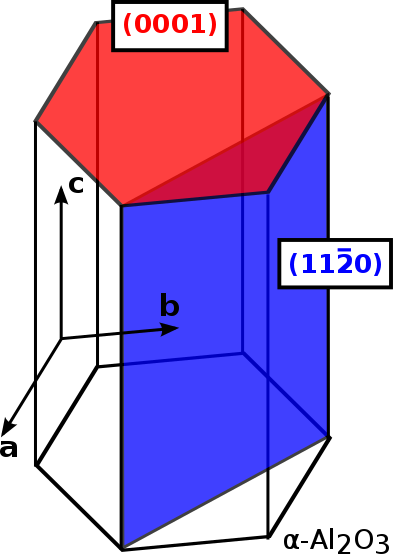
\includegraphics[width=0.30\textwidth]{figures/al2o3-crystal.png}}
             \quad
             %add desired spacing between images, e. g. ~, \quad, \qquad, \hfill etc. (or a blank line to force the subfigure onto a new line)
    \subfigure[(11\=20), top view]{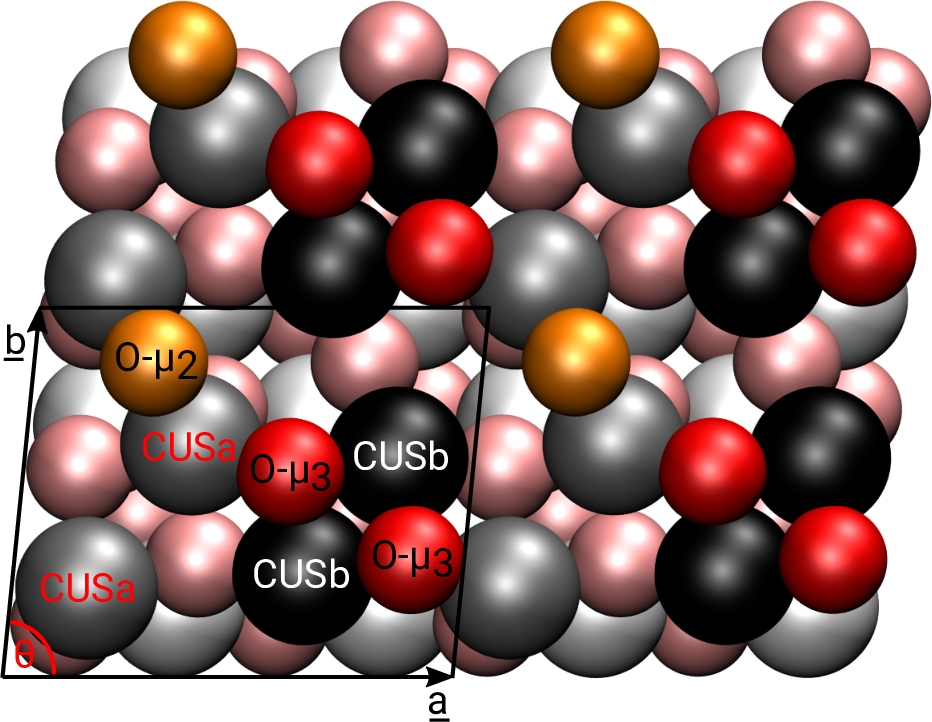
\includegraphics[width=0.30\textwidth]{figures/11-20/supercell_opt.png}}
             \quad
             %add desired spacing between images, e. g. ~, \quad, \qquad, \hfill etc. (or a blank line to force the subfigure onto a new line)
    \subfigure[(11\=20), side view]{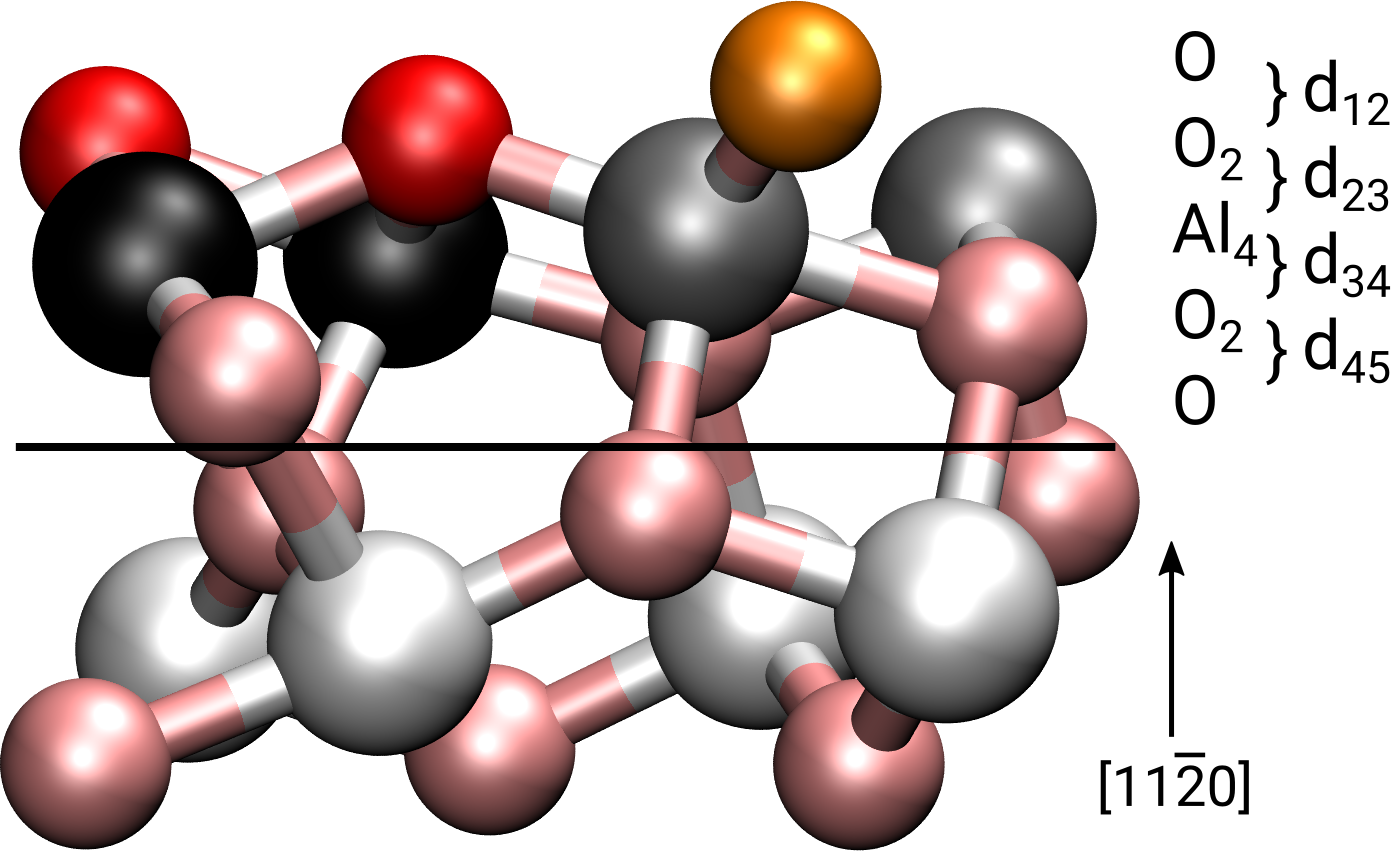
\includegraphics[width=0.30\textwidth]{figures/11-20/uc_opt.png}}
             \caption{The crystal cut of $\upalpha$-Al$_2$O$_3$, (a) schematic compared to the (0001) surface, (b) a top view of the geometry optimized unit cell with the nomenclature of the surface atoms and (c) as a side view showing the different atomic layers, see main text.}
            \label{abb:crystal_11-20}
\end{figure}
\begin{figure}[!h]
    \centering
    \includegraphics[width=0.80\textwidth]{figures/11-20/cell_sizes.pdf}
             \caption{Side view for the different cell sizes from left to right 10, 15, 20 and 25 layers. Surface atoms are shown in the color code as used before.}
            \label{abb:cell_sizes}
\end{figure}
$\vec{k}$-point tests were done for 5 different grid sizes from $1\times 1\times 1$ to $5\times 5\times 1$. In contrast to the even grid sizes, the odd ones contain the $\Gamma$-point and therefore are favorable. It was shown that the $3\times 3\times 1$ grid is already converged with respect to the energy of the clean surface, see Fig.~\ref{abb:11-20-kpointsampling}.
\begin{figure}[!h]
\centering
 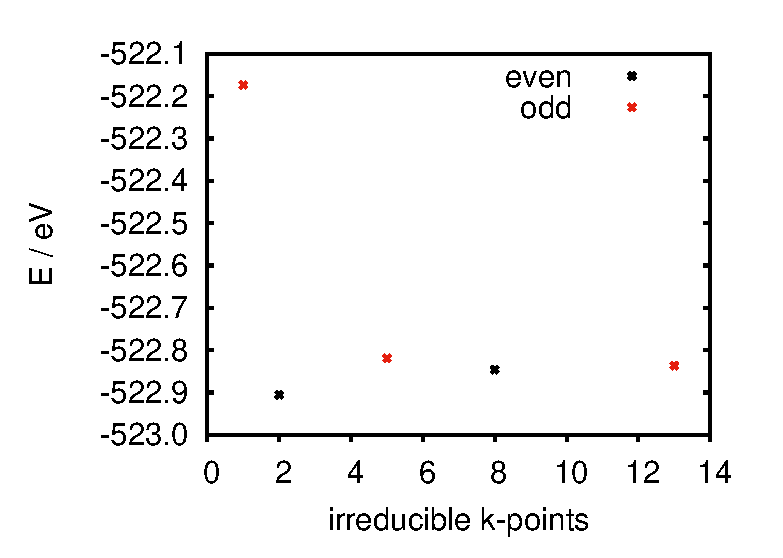
\includegraphics[width=0.4\textwidth]{figures/11-20/irreducibles-E.eps}
   \caption{Sampling of the $\vec{k}$-points, shown is the energy of the super cell with respect to the number of irreducible $\vec{k}$-points. The even values correspond to the $2\times 2 \times 1$ (2 irreducibles) and $4\times 4\times 1$ (8 irr.), whereas the odd, that contain the $\Gamma$-point, are described by $1\times 1\times 1$ (1 irr.), $3\times 3\times 1$ (5 irr.) and $5\times 5\times 1$ (13 irr.).}
            \label{abb:11-20-kpointsampling}
\end{figure}
\\
Starting from this supercell approach there are 16 CUS Al-atoms (cordinatively unsaturated sites), these have less bonds than the aluminum atoms in the bulk structure since the surface layers has to be  depleted. These atoms are very interesting for adorbate molecules/atoms, because these atoms are electron rich and can be addressed for adsorption. If these 16 atoms are covered with adsorbates, here water, we get the system with 1 mono layer (ML). But one has to keep in mind the difference between these 16 surface atoms and the number of potential adsorbates: one monolayer is not built by 16 adsorbates since not all 16 CUS positions can be covered, but only 12, as is shown later (bridging water adsorption).
\\
As is shown with different colors in figure \ref{abb:crystal_11-20} (b) and (c), the system consists of different types of CUS Al atoms with different coordination neighborhood and 2 different types of oxygen atoms, 2-fold and 3-fold coordinated. The Alumina atoms have the same number of oxygen neighbor atoms but differ slightly in the arrangement of their neighbors and the distance in the relaxed structure, but the oxygen atoms in fact differ by the number of neighbors. In this work, the black spheres denote the CUSb atoms, the grey ones depict the CUSa, the twofold coordinated oxygen atoms (O-$\mu_2$) are shown in yellow and the threefold coordinated (O-$\mu_3$) in red. Atoms of the underlying layers are illustrated in pale colors, light grey for alumina and pale red for oxygen.

\section{Structure Search}\label{structure_search11-20}
{\color{red} acid base character of the adsorption, undercoordination of the alumina sites, bidentate adsorption, different types of Al and O cause large variety of possible adsorption sites}
First a low coverage regime was investigated: 1 water molecule per $2\times 2$ supercell, which equals a coverage of 1/12. It was put on different positions on the surface and let relax. We found 1 molecular minimum and several dissociated species including both CUS and oxygen types, for adsorption energy and Gibb's free energy results see Table \ref{tab:ads_1water}. There is also one metastable molecular species that seems more stable than the found molecular minimum, but since there is one imaginary mode displaying the movement of the proton towards the dissociated species this cannot be classified as a stable minimum.
The adsorption energy is defined by equation \ref{eq:Eads} as the energy of the adsorbed system compared to the energies of the clean surface and the isolated water molecule:
\begin{equation}\label{eq:Eads}
 E_\textrm{ads}=E_\text{ads. species}-(E_\text{free water molecule}+E_\text{surface}).
\end{equation}

The nomenclature for the adsorption sites that is used in the following gives at first the type of Al site where the OH-residue (OH$^-$) is adsorbed and at second place the oxygen type where the H(/H$^+$) is adsorbed (OH-site$\parallel$H-site). The notation with the $\prime$ that will occur later denotes greater distances between the residues.
\begin{table}[!ht]
  \centering
 \caption{{\textit change text! Adsorption energies as calculated from equation \ref{eq:Eads}
 for molecular and (singly) dissociated water on $\upalpha$-\ce{Al2O3}(11\=20)
according to periodic PBE+D2 calculations. Also the corresponding 
adsorption free energies $G_\textrm{ads}$ at $130$, $300$ and $400\,$K defined 
analogously are also given. The three most stable configurations are in bold. All 
energies are given in eV.} 
\vspace*{.2cm} 
  }
  \begin{tabular}{cl|cccc}
   \multicolumn{2}{c|}{Adsorbed Species}  & $E_\text{ads}$ & $G_\text{ads, 130 K}$  &  $G_\text{ads, 300 K}$  & $G_\text{ads, 400 K}$ \\
\hline
\multirow{1}{*}{molecular} & CUSb          &   -1.78  &-1.60 & -1.51  & -1.46 \\
  \hline
 \multirow{6}{*}{dissociated} & \textbf{inter-CUSa||O-$\mu_2$} & \textbf{-2.50} &-2.27 & -2.16 & -2.09 \\
  & inter-CUSa||O-$\mu_3$ & -1.67 &-1.44 &-1.33 & -1.27 \\
  & \textbf{CUSb||O-$\mu_2$} & \textbf{-2.28} & -2.12& -2.03 &-1.97  \\
 & CUSb||O-$\mu_3$ & -1.19 &-1.05 &-0.98 & -0.95 \\%Cb3_other
 & \textbf{inter-CUSb||O-$\mu_2$} & \textbf{-2.09} &-1.88 &-1.80 & -1.76 \\
 & inter-CUSb||O-$\mu_3$ & -1.89 &-1.71 & -1.63 & -1.58 \\
  \end{tabular}
  \label{tab:ads_1water}
\end{table}
\begin{figure}[!ht]
 \centering
\subfigure[CUSb]{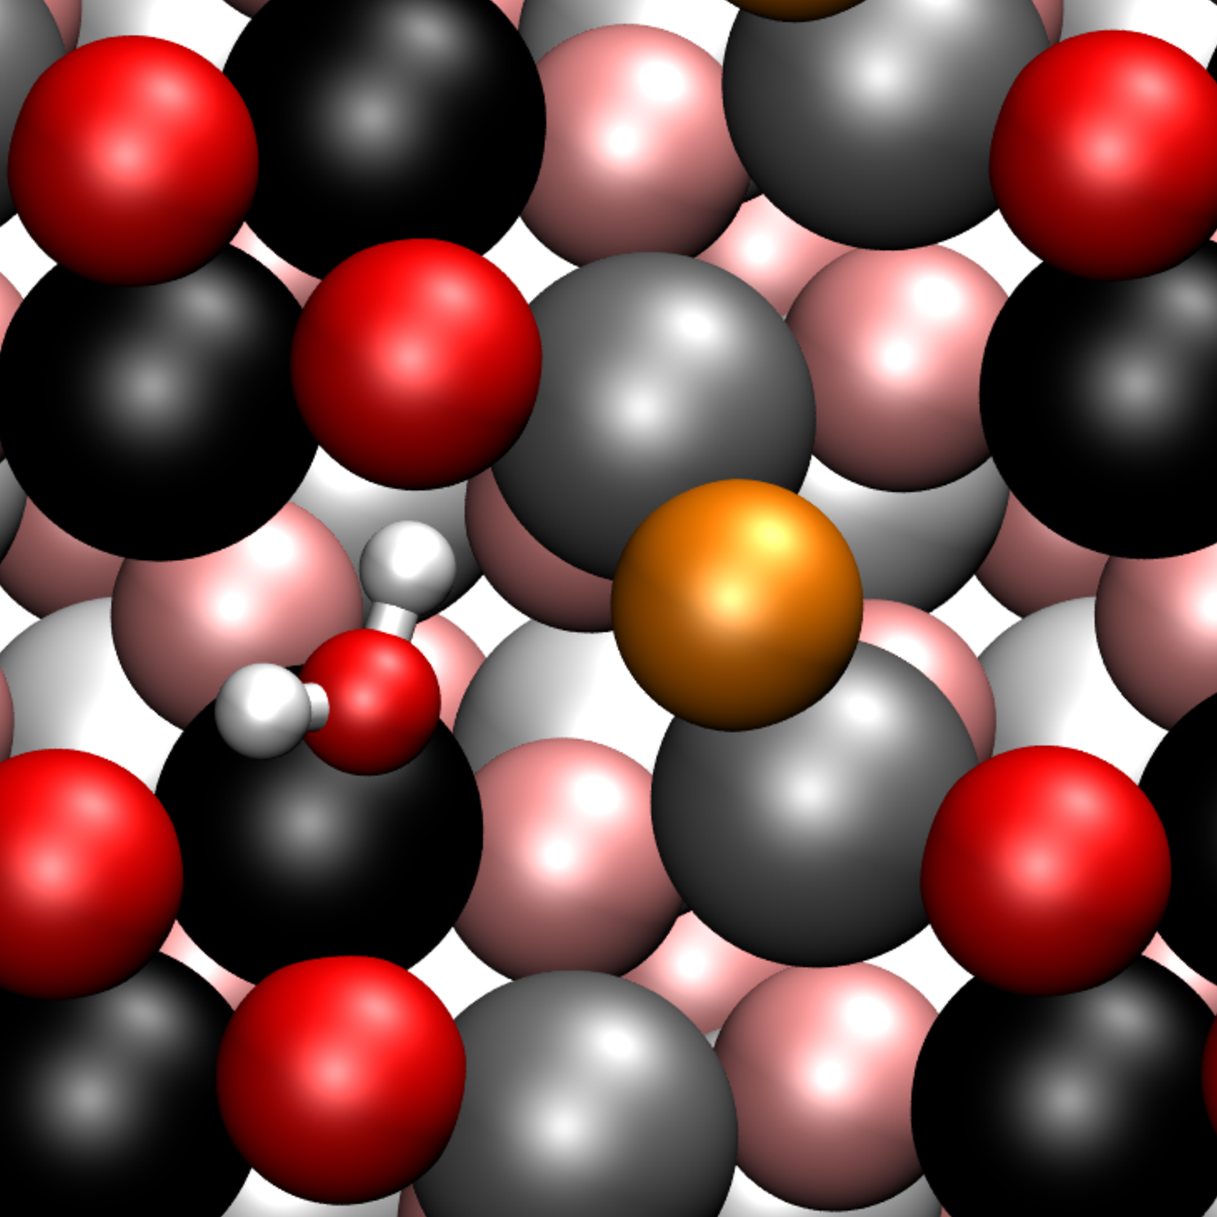
\includegraphics[width=0.2\textwidth]{figures/11-20/test-Cb.pdf}}
 \quad\quad
 \subfigure[inter-CUSa||O-$\mu_2$]{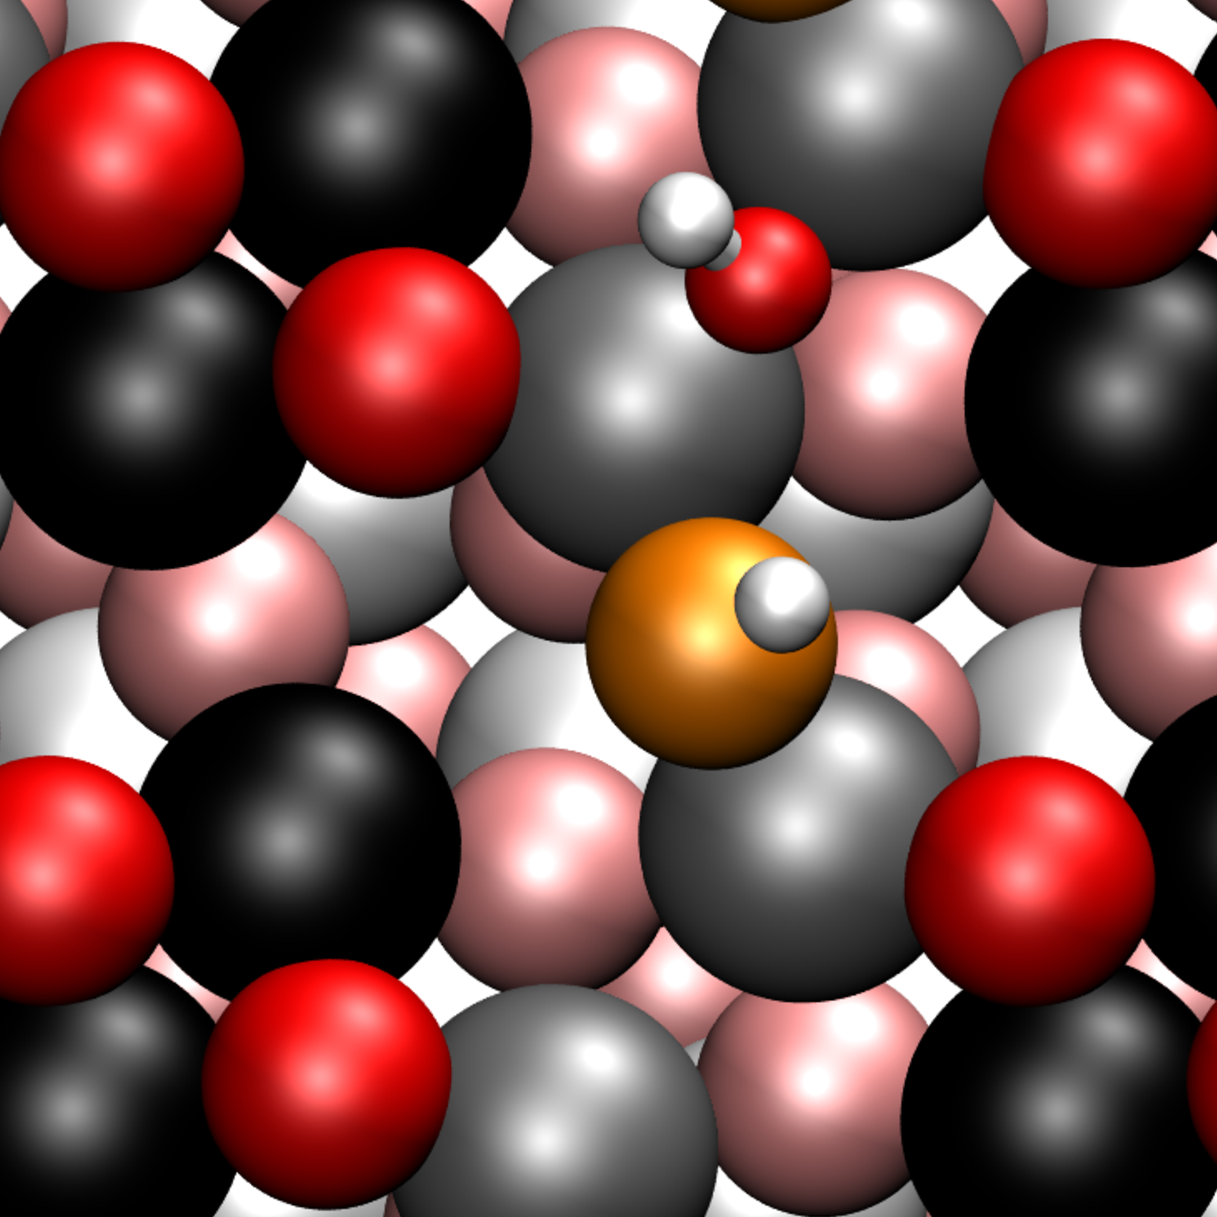
\includegraphics[width=0.2\textwidth]{figures/11-20/test-iCa2.pdf}}
  \quad
\subfigure[CUSb||O-$\mu_2$]{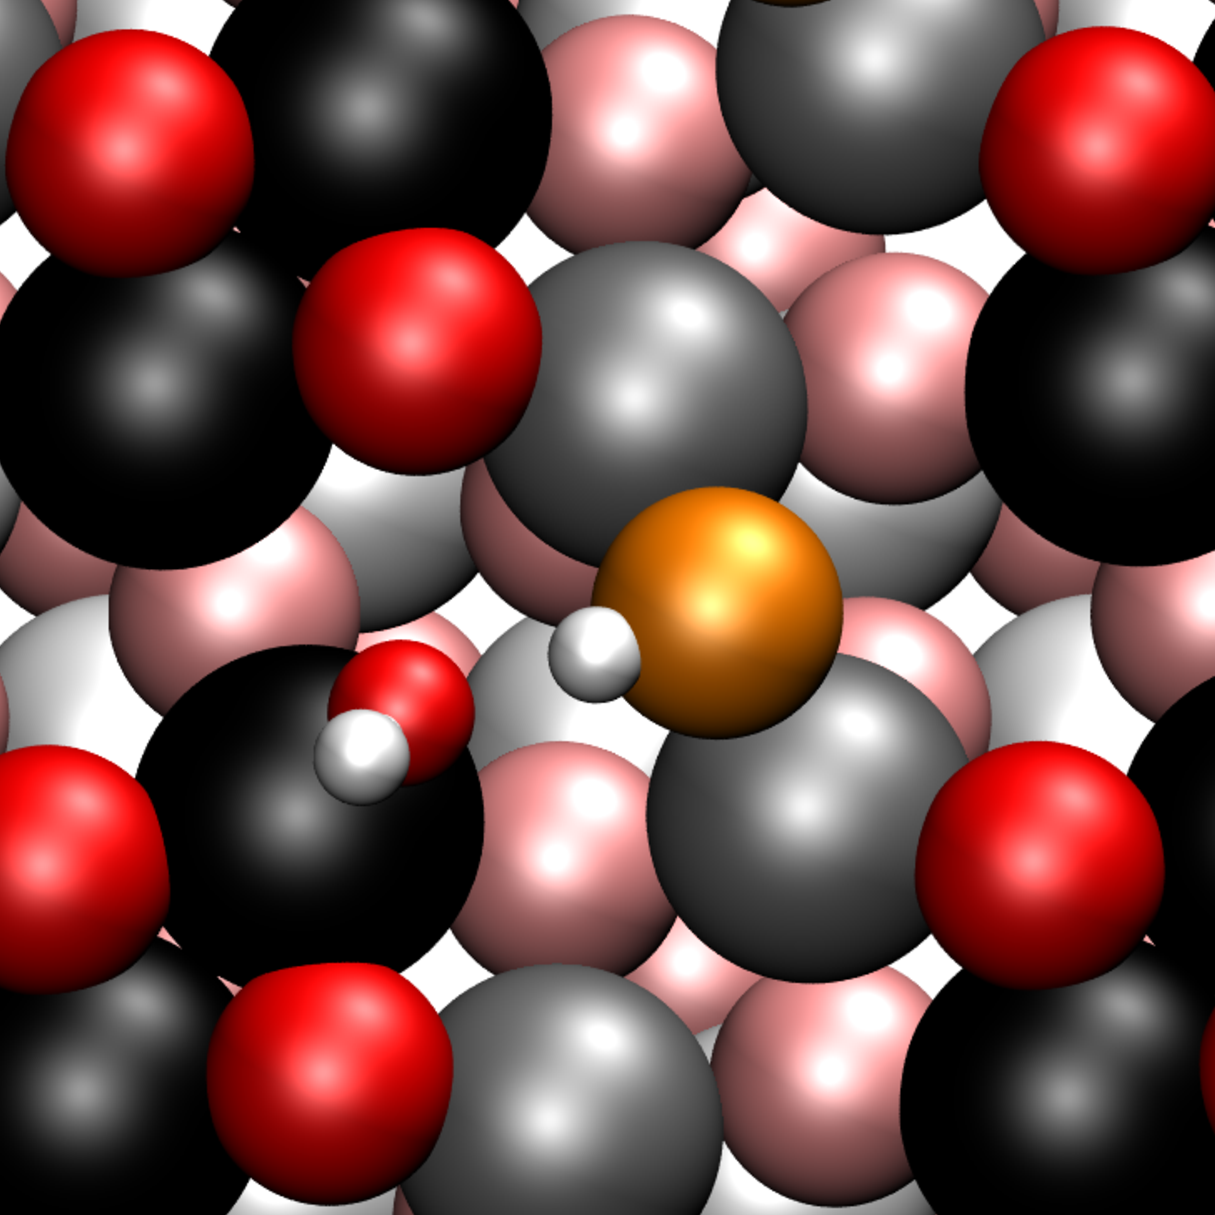
\includegraphics[width=0.2\textwidth]{figures/11-20/test-Cb2.pdf}}
 \quad
\subfigure[inter-CUSb||O-$\mu_2$]{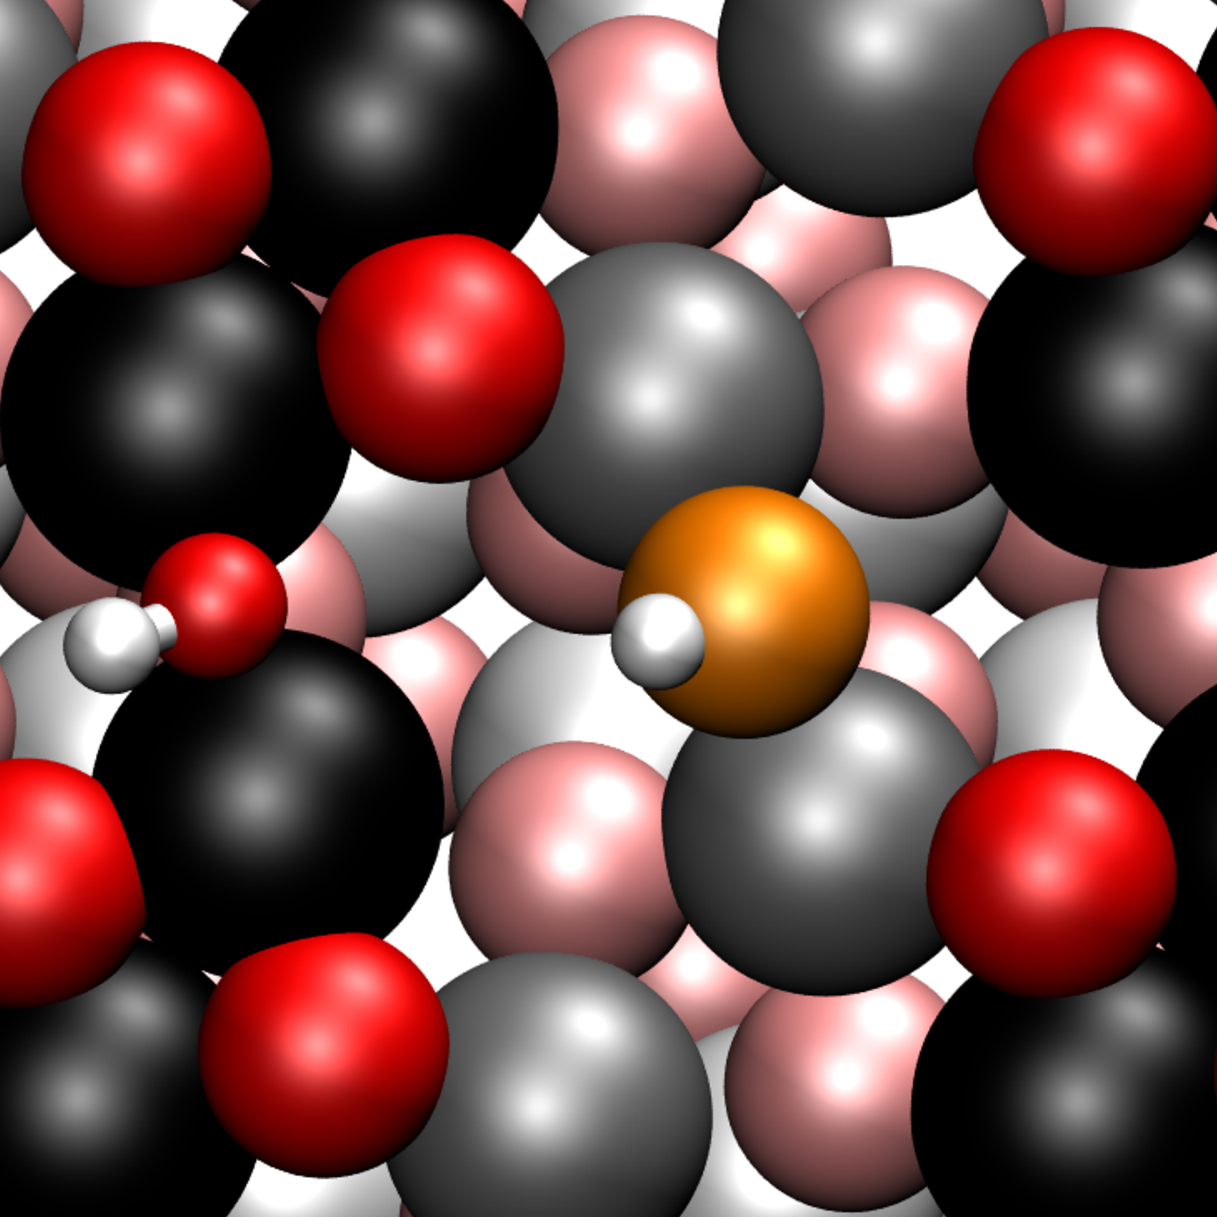
\includegraphics[width=0.2\textwidth]{figures/11-20/test-iCb2.pdf}}
\quad
\subfigure[inter-CUSa||O-$\mu_3$]{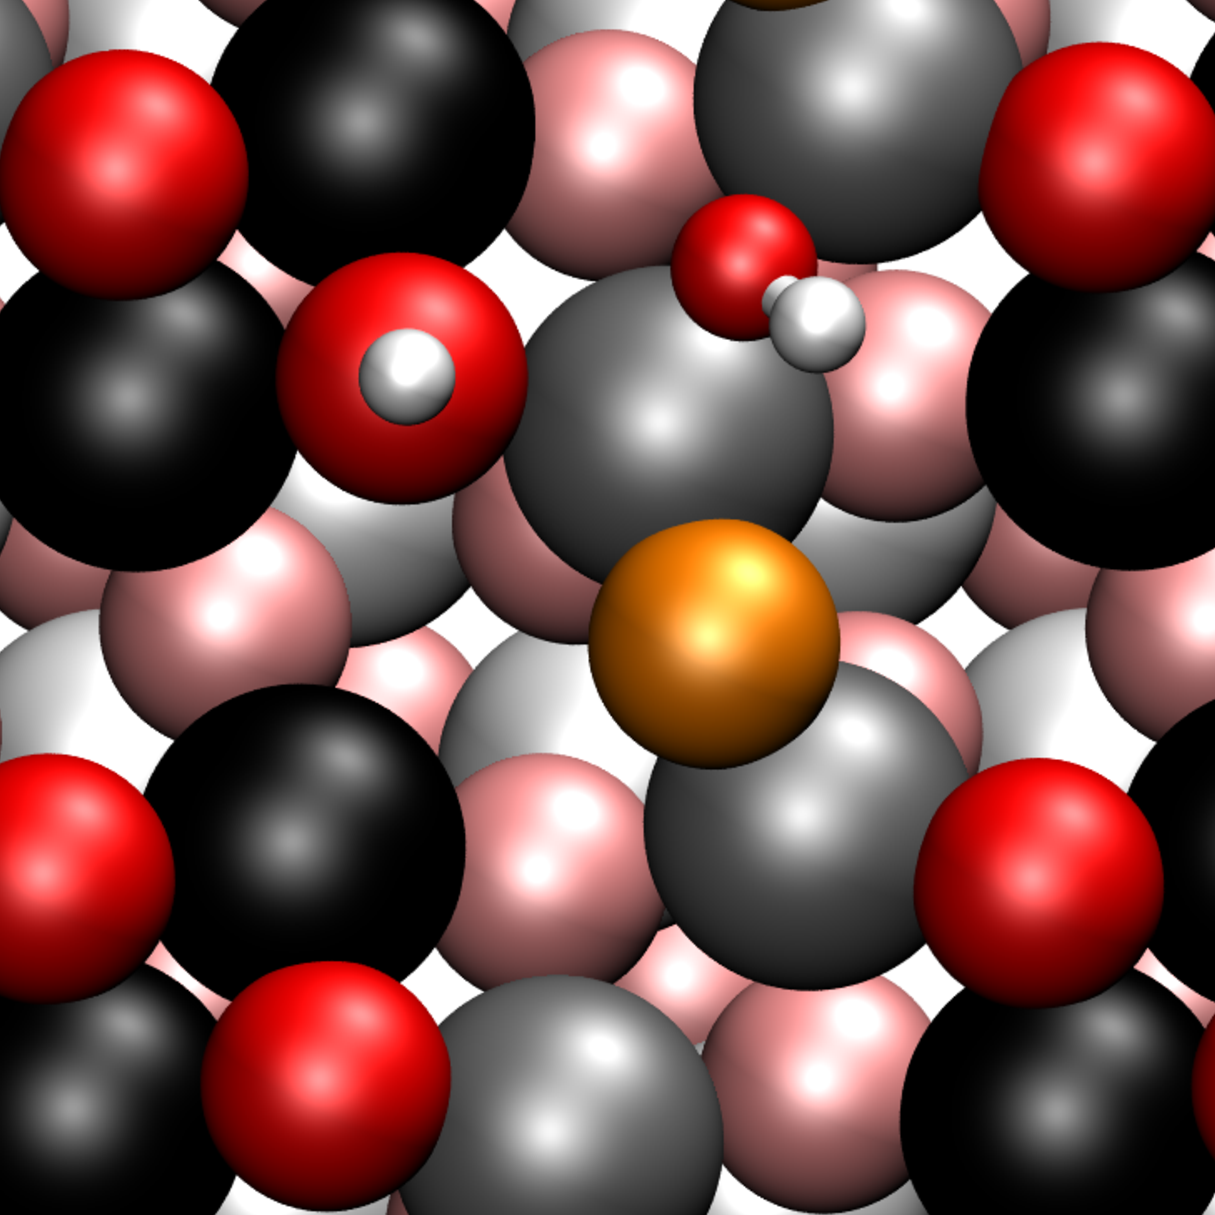
\includegraphics[width=0.2\textwidth]{figures/11-20/test-iCa3.pdf}}
 \quad
\subfigure[CUSb||O-$\mu_3$]{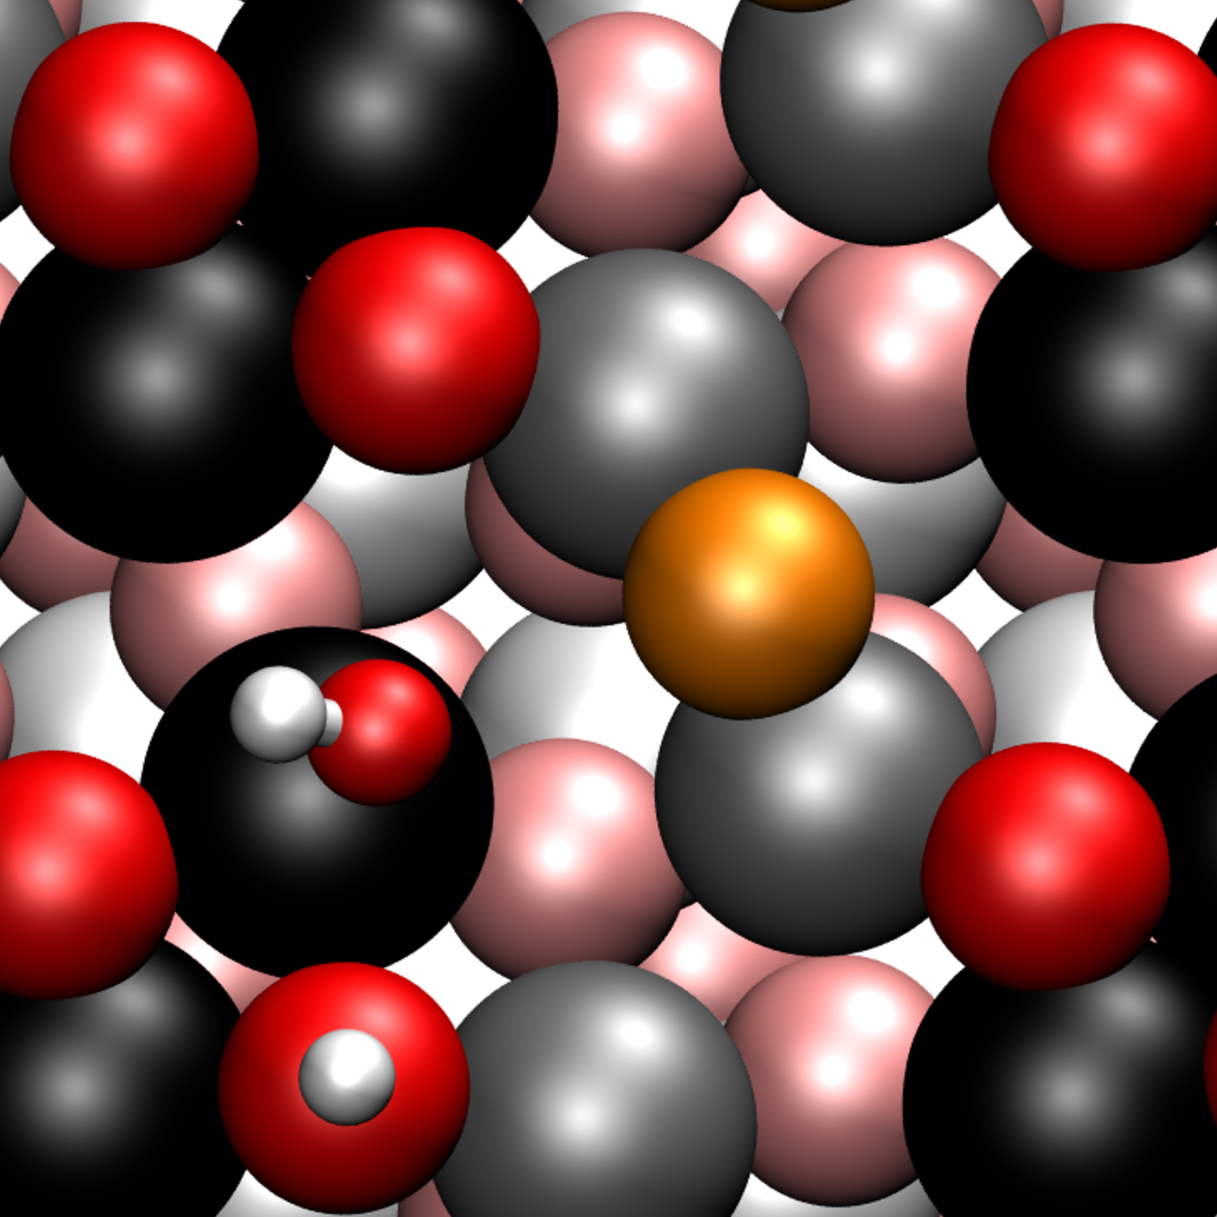
\includegraphics[width=0.2\textwidth]{figures/11-20/test-Cb3.pdf}}
 \quad
\subfigure[inter-CUSb||O-$\mu_3$]{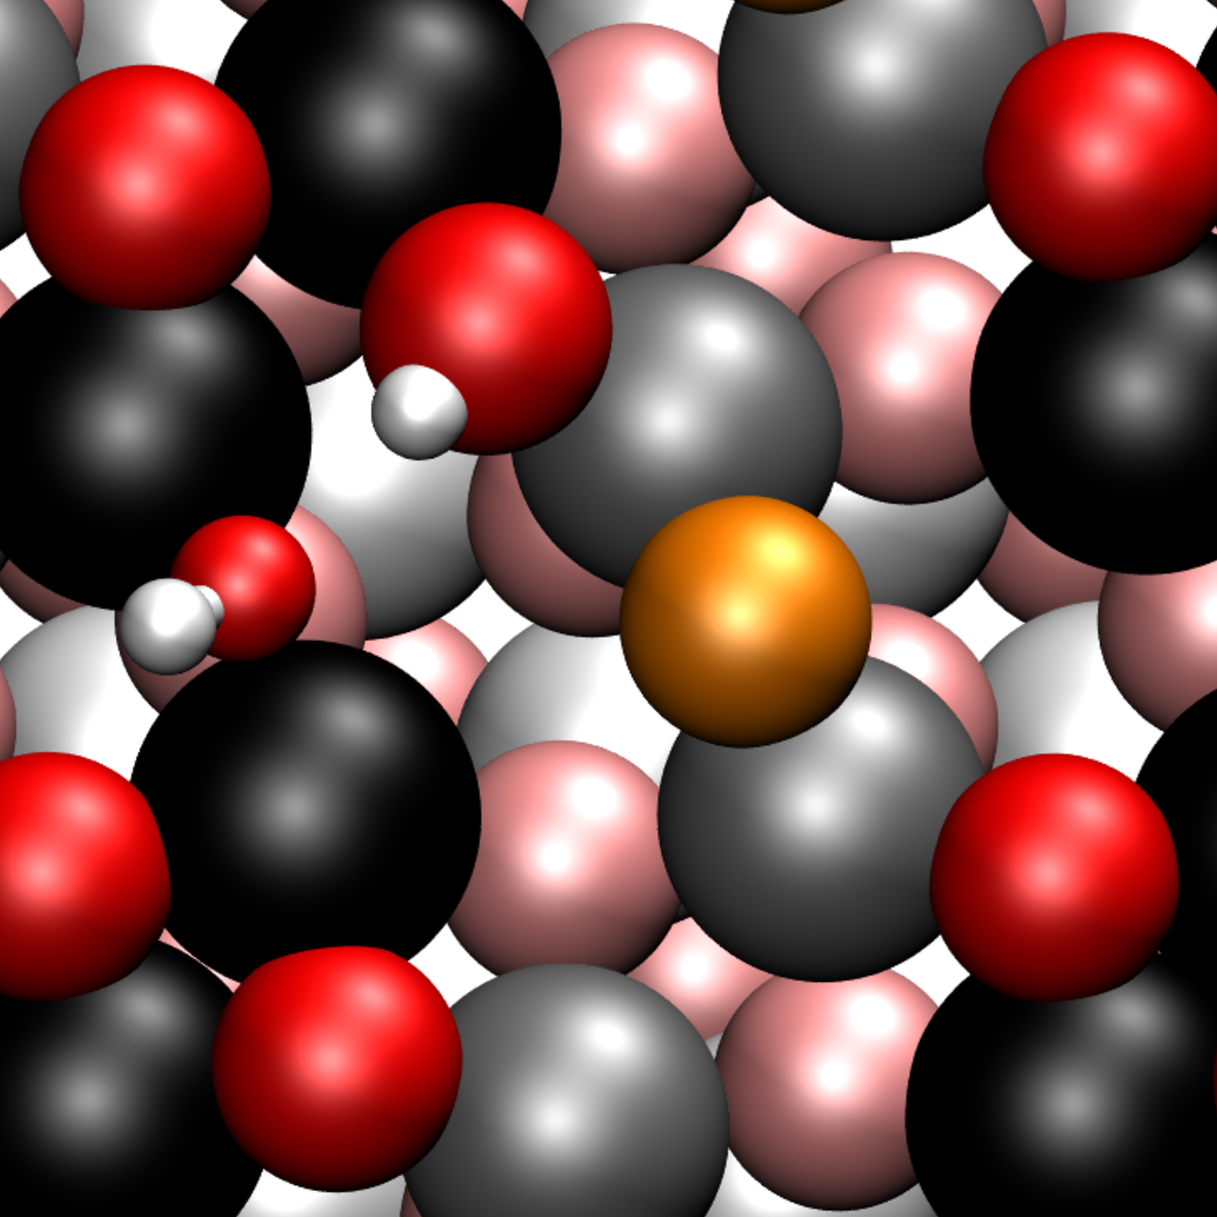
\includegraphics[width=0.2\textwidth]{figures/11-20/test-iCb3.pdf}}
 \caption{{\textit change text! Adsorption geometries for molecular (a) and (six) dissociated water 
molecules ((b)-(g)) are shown, as obtained by periodic PBE+D2. The most favorable 
molecularly and dissociatively adsorbed configurations are shown. This means that 
we show nearest neighbor structures only (see text). The color code is the same 
as in Figure \ref{abb:crystal_11-20}(b) and (c), CUSa grey, CUSb black, O-$\mu_2$ yellow and O-$
\mu_3$ red; Hydrogen is displayed in white, subsurface layers are in pale colors.}}
        \label{abb:ads-geoms}
 \end{figure}
The molecular minimum is substantially less stable than the dissociated species. On the contrary, the dissociated water is very stable, also in comparison with the more stable surface cuts (0001) and (1\=102) that were investigated before in our group by Dr. Jonas Wirth\cite{C6CP01397J,WirthJPCC2012}. Dissociated species, where the proton is located at a twofold coordinated surface oxygen is far more stable than the corresponding systems where the threefold coordinated is occupied, since the higher negative charge and the higher basicity of such a twofolded oxygen atom in comparison with the more saturated threefold coordinated O-$\mu_3$ oxygen atom. Also the adsorption of OH at an inter-CUSa site is more favorable than at a CUSb site, because the former corresponds to a site where in the bulk system another oxygen atom would be situated, which is not the case for the CUSb position.
\\
Dissociated species in direct neighborhood as shown in Table \ref{tab:ads_1water} and figure \ref{abb:ads-geoms} are more stable than those where the proton and the OH residue are further apart (see Table \ref{tab:ads_1waterfurther}), because the OH residue has a stabilizing effect on the H. In the table one can see, that the inter-CUSb||O-$\mu_3^{\prime\prime}$-species is more stable than the species inter-CUSb||O-$\mu_3^\prime$. This is due to the fact, that the periodic conditions lead to the decrease of the distance between OH groups again, so that between 3 neighboring OH groups in the O-$\mu_3^\prime$ system the distances are $0.68$ and $0.77\,$nm, whereas in the O-$\mu_3^{\prime\prime}$ system the distances are $0.93$ and $0.62\,$nm, where the latter one is closer by, so there is more stabilization. For examples of further diffusion reactions, see chapter \ref{reactions}.
\begin{table}[!ht]
  \centering
 \caption{Comparison of next neighbor dissociated species and species where OH and H are further apart. 
\vspace*{.2cm} 
  }
  \begin{tabular}{cc}
  Adsorbed Species  & $E_\text{ads} [eV]$  \\
   inter-CUSa||O-$\mu_3$ & -1.67 \\
   inter-CUSa||O-$\mu_3^\prime$ & -1.42 \\\hline
   inter-CUSb||O-$\mu_3$ & -1.89\\
   inter-CUSb||O-$\mu_3^\prime$ & -1.16\\
   inter-CUSb||O-$\mu_3^{\prime\prime}$ & -1.22\\
  \end{tabular}
  \label{tab:ads_1waterfurther}
\end{table}
\\
Systems with more layers were also studied and the adsorption energy results are shown in Table \ref{tab:eads_layers}. Basically the results don't change much with increasing slab size. The molecular species is still less stable than most of the dissociated species, inter-CUSa$\parallel$O-$\mu_2$ is the most stable structure through all the sampled systems, inter-CUSb$\parallel$O-$\mu_2$ and CUSb$\parallel$O-$\mu_2$ change their stability depending on the number of layers but still are some orders of magnitude less probable than inter-CUSa$\parallel$O-$\mu_2$. Dissociated systems occupying the threefold coordinated surface oxygen atom are in the same stability order, relatively to each other. For higher number of layers, the inter-CUSb gets more favourable than CUSb, both for O-$\mu_2$ and O-$\mu_3$. This might be due to less interaction between neighboring oxygen atoms with the inter-CUSb adsorbed OH group.
  \begin{table}[!ht]
  \centering
  \caption{Adsorption energies calculated from equation \ref{eq:Eads} for molecular and dissociated species for different vertical slab sizes. All values are in eV.}
 \begin{tabular}{l|cccc}
 System                     & 10 layers& 15 layers& 20 layers&  25 layers \\\hline
CUSb                                    &-1.78 &-1.80     &-1.81     &-1.83      \\\hline
\textbf{inter-CUSa$\parallel$O-$\mu_2$}    &\textbf{-2.50} &-2.46 &-2.54 &-2.56  \\
inter-CUSa$\parallel$O-$\mu_3$          &-1.67 &-1.67 &-1.78 &-1.80 \\
\textbf{CUSb$\parallel$O-$\mu_2$}          &\textbf{-2.28} &-2.35 &-2.36 &-2.35 \\
CUSb$\parallel$O-$\mu_3$                &-1.19 &-1.71 &-     &-      \\
\textbf{inter-CUSb$\parallel$O-$\mu_2$}    &\textbf{-2.09} &-2.43 &-2.48 &-2.36  \\
inter-CUSb$\parallel$O-$\mu_3$          &-1.89 &-1.59 &-1.65 &-2.09 
\label{tab:eads_layers}
\end{tabular}
 \end{table}
This brings the point into attention that the system is already converged for the 10-layer slab referring to adsorption energies (and also vibrational OH/OD frequencies as can be seen later in section \ref{nma}).
\\
Also systems with a higher water coverage were considered, some cases for 2 water molecules, 4 inter-CUSa$\parallel$O-$\mu_2$ and a fully covered supercell, for these systems also normal mode analyses were done to get vibrational spectra, see also chapter \ref{phonons}.

The stability of those species with higher water coverage is defined as
\begin{equation}
 E_\textrm{ads}=E_\text{ads. species}-(E_\text{free water molecule}\times n+E_\text{surface}),
\end{equation}
 with $n$ being the number of water molecules adsorbed on the surface. In Table \ref{tab:higher_water}, the adsorption energies are given.
\begin{table}[!ht]
  \centering
 \caption{Adsorption energies in eV for higher water coverages. For comparison in the third column the added energies for singly adsorbed water are shown.
\vspace*{.2cm} 
  }
  \begin{tabular}{lcc}
  Adsorbed Species  & $E_\text{ads}$ &isolated species \\
   CUSb(mol)+CUSb||O-$\mu_2$ & -4.57 & -4.06\\
   inter-CUSa||O-$\mu_2$+CUSb||O-$\mu_2$ & -4.77 & -4.78\\
   2inter-CUSa||O-$\mu_2$& -4.84 &-5.0 \\\hline
   4inter-CUSa||O-$\mu_2$ & -9.55 & -10.0\\\hline
   12H$_2$O & -23.39& $a$\tnote{a} \\
  \end{tabular}
  \label{tab:higher_water}
  \begin{tablenotes}\footnotesize 
    \item[a] $a$ One can not distinguish exactly, but there are 4 inter-CUSa-OD groups, 8 CUSb-OD groups, 8 O-$\mu_3$ and 4 O-$\mu_2$ OD groups, hence one can not calculate a sum of the isolated species.
  \end{tablenotes}

\end{table}
Comparing these results for the higher coverages to results with only one adsorbate, just by adding the adsorption energy one can see the following (see also column 3 in Table \ref{tab:higher_water}):
For all systems the added energy of the singly adsorbed species is more stable than the doubly adsorbed water systems. Instead of stabilizing the whole system, they are destabilized by the adsorption neighborhood, even in structures that contain hydrogen bonds.
{\color{red} do neighbors stabilize molecular adsorption?? In Phonon paper, Eads(Cb+Cb2)=-4.57eV, sum of the two individually is -4.06eV, so there is in fact a stabilizing effect!, For inter-CUSa$\parallel$O-$\mu_2$+CUSb$\parallel$O-$\mu_2$ there is no effect and for inter-CUSa$\parallel$O-$\mu_2$inter-CUSa$\parallel$O-$\mu_2$, there is clear destabilization!
\\ What is the respective coverage? 0.xyML}

\section{Reactions and Microkinetic Model}\label{reactions}
Based on the minimum structures one has to identify reaction pathways to fully understand the reactivity of a system, so we utilize the NEB method including Climbing Image to search for transition states between the minima. We examined 3 different types of reactions: dissociation from the molecular minimum, as well as OH- and H-diffusion. The dissociation reactions are named D, diffusion reaction with Df-OH and Df-H, respectively, in Table \ref{tab:reaction-rates} and figures \ref{mep} and \ref{mep2}. In reference {\color{red} 11-20paper} only some reactions were introduced, additional reactions paths are given here.
\\
We investigated 5 different dissociation reactions. The two that were already shown in the publication {\color{red} 11-20paper} are the reactions from CUSb to the twofold coordinated oxygen (D-a) and one to the threefold coordinated O (D-b). One additional dissociation starts from the metastable inter-CUSa molecular structure that is, as was shown before, no minimum structure and goes to the most stable species inter-CUSa$\parallel$O-$\mu_2$ (D-c). 2 further dissociation reactions converged but showed a two step process and are therefore not interesting in the first place (these reactions are CUSb$\rightarrow$inter-CUSa$\parallel$O-$\mu_2$ and CUSb$\rightarrow$inter-CUSb$\parallel$O-$\mu_2$ and both went via the dissociated CUSb$\parallel$O-$\mu_2$ intermediate {\color{blue} put them into appendix?}).
As can be seen from chapter \ref{structure_search11-20} (Table \ref{tab:ads_1water}), the molecular minimum CUSb is very low in stability compared to the dissociated minima. The reaction D-a leads from the molecular minimum at CUSb to the twofold coordinated CUSb$\parallel$O-$\mu_2$:
 \begin{equation}
 \text{H$_2$O(CUSb)} \rightarrow \text{OH(CUSb)} + \text{H(O-$\mu_2$)} \tag{D-a}
      \label{dissa}
\end{equation}
The barrier is very low, about $0.002\,$eV as one can see from Table \ref{tab:reaction-rates} and figure \ref{mep}(a), hence the reaction rate constant is very high, in the range of $k_{\text{300K}}=10^{12}\,$s$^{-1}$. This low barrier might be due to underestimation of barrier heights with the used functional PBE (compare chapter {\color{red} citation x}, \ref{theorybeyond}).
\\ 
For the other dissociation reaction D-b from CUSb to CUSb$\parallel$O-$\mu_3$, there is no barrier found at all, the reaction pathway shows simply an upgoing path in energy without any barrier, since the molecular minimum is by $0.15\,$eV more stable than the dissociated structure on CUSb$\parallel$O-$\mu_3$. Thus, no reaction rate constant can be calculated.
\begin{equation}
  \text{H$_2$O(CUSb)} \rightarrow \text{OH(CUSb)} + \text{H(O-$\mu_3$)} \tag{D-b}
      \label{dissb}
\end{equation}
A further dissociation D-c from the metastable inter-CUSa species also shows no barrier, probably because the educt is no stable minimum and because the product is much more stable:
\begin{equation}
  \text{H$_2$O(inter-CUSa)} \rightarrow \text{OH(inter-CUSa)} + \text{H(O-$\mu_2$)} \tag{D-c}
      \label{dissc}
\end{equation}
On the other hand reaction D-b does also not show a barrier, so it remains unclear whether it is due to methodology or the barrier is too low to be detected with the settings applied for the calculations.
\\
Apart from dissociation that is highly favoured on this surface cut compared to more stable alumina surfaces, diffusion reactions starting from the dissociated species are important for understanding processes.
The OD diffusion reaction Df-OH-a moves from CUSb$\parallel$O-$\mu_2$ to the inter-CUSb position, which is relatively fast for OD diffusion reactions compared to the reactions at other alumina surfaces {\color{red} cite Jonas}.
\begin{equation}
 \text{OH(CUSb)} + \text{H(O-$\mu_2$)} \rightarrow \text{OH(inter-CUSb)} + \text{H(O-$\mu_2$)} \tag{Df-OH-a}
     \label{diffOHa}
\end{equation}
In this special reaction, the OH residue diffuses from an on top CUS position into a gap between two CUSb atoms, so that there is not much repulsion with neighboring surface oxygen atoms and other CUS atoms nearby during the diffusion. Also the distance that has to be bridged is very small. The barrier height equals $0.35\,$eV and the corresponding rate constant $k_{\text{300K}}=1.88\times 10^6$s$^{-1}$.
In contrast to that the real CUS-to-CUS reaction Df-OH-b that is much slower. It is a diffusion from CUSb to inter-CUSa with the hydrogen residue staying at an O-$\mu_2$ position. This barrier is with $1.07\,$eV relatively high and leads to $k_{\text{300K}}=2.41\times 10^{-6}$s$^{-1}$.
\begin{equation}
 \text{OH(CUSb)} + \text{H(O-$\mu_2$)} \rightarrow \text{OH(inter-CUSa)} + \text{H(O-$\mu_2$)} \tag{Df-OH-b}
     \label{diffOHb}
\end{equation}
This is still faster than OH diffusion reaction for the (0001) alumina surface ({\color{red} cite Jonas} and compare to doctoral thesis of Dr. Jonas Wirth, UP 2016), where the rates constant $k_{\text{300K}}=4\times 10^{-45}$s$^{-1}$.
For the (1\=102) surface there was no OH diffusion calculated, but the corresponding H$_2$O diffusion process is around $k_{\text{300K}}=1.4\times 10^{-3}$s$^{-1}$, whereas the H$_2$O diffusion process for the (0001) surface is in the range of $k_{\text{300K}}=8\times 10^{-3}$s$^{-1}$, too. For the (11\=20) surface no H$_2$O diffusion reactions can be observed due to the instability of the molecularly adsorbed species that would rather dissociate than diffuse.
\\
A larger variety can be achieved when looking at H diffusion reactions. The different types of surface oxygen atoms and also the distances between OH and H residue make differences in the observed reactions.
{\color{blue} As seen before, the hydrogen is preferably found on the twofold coordianted oxygen atom, but the reaction to a neighboring threefold coordinated oxygen is possible and opens the gate to structures with greater proximity. The reaction takes place with the OH residue being on a CUSb site:
\begin{equation}
 \text{OH(CUSb)} + \text{H(O-$\mu_2$)} \rightarrow \text{OH(CUSb)} + \text{H(O-$\mu_3$)} \tag{Df-H-a}
     \label{diffHa}
\end{equation}
The reaction shows a barrier heigt of $0.95\,$eV, but the NEB transition state has no imaginary frequency so that no rate can be derived, although the NEB path clearly shows a smooth barrier profile.}
An analogue reaction starting from the most stable inter-CUSa$\parallel$O-$\mu_2$ to the threefold coordinated oxygen is reaction Df-H-b:
\begin{equation}
 \text{OH(inter-CUSa)} + \text{H(O-$\mu_2$)} \rightarrow \text{OH(inter-CUSa)} + \text{H(O-$\mu_3^\prime$)} \tag{Df-H-b}
     \label{diffHb}
\end{equation}
the barrier of the free energy is $1.50\,$eV, rate constant at $300\,$K of $4.90\times 10^{-13}$s$^{-1}$. This process is so unlikely because a less favored O-$\mu_3$ position is occcupied and this position is also less stabilized by reason of the greater distance of OH$_{\text{surf}}$ and OH$_{\text{ads}}$ groups. This reaction increases the distance to a position further away than next neighbor.
As mentioned before, the nomenclature for these structures uses different amounts of primes ($\prime$) to display the distance.
A similar reaction for the OH sitting on inter-CUSb and the hydrogen being adsorbed on an O-$\mu_2^\prime$ position, diffusing further away to O-$\mu_3^{\prime\prime}$, which is less in stability:
\begin{equation}
 \text{OH(inter-CUSb)} + \text{H(O-$\mu_2^{(\prime)}$)} \rightarrow \text{OH(inter-CUSb)} + \text{H(O-$\mu_3^{\prime\prime}$)} \tag{Df-H-c}
     \label{diffHc}
\end{equation}
The free energy barrier is relatively high with $1.30\,$eV leading to a rate constant $k_\textrm{300K}=9.96\times 10^{-1}$s$^{-1}$. The $^\prime$ in the equation above is set in parantheses because it is the nearest possible O-$\mu_2$ position, but not the nearest possible distance from the OH$_\textrm{ads}$.

Going one step further from reaction Df-H-d, the last reaction leads to the position where OH and H have the greatest possible distance with the applied periodic bounding conditions:
\begin{equation}
 \text{OH(inter-CUSb)} + \text{H(O-$\mu_3^{\prime\prime}$)} \rightarrow \text{OH(inter-CUSb)} + \text{H(O-$\mu_3^{\prime\prime\prime}$)} \tag{Df-H-d}
     \label{diffHd}
\end{equation}
With an energy barrier of $0.94\,$eV the rate at $300\,$K is $1.1\times 10^{-3}$s$^{-1}$.
\\
{\color{blue} Possible path from inter-CUSb$\parallel$O-$\mu_3$ to O-$\mu_3^\prime$ to O-$\mu_3^{\prime\prime}$and to the furthest possible O-$\mu_3^{\prime\prime\prime}$. The first reaction was calculated but did not converge for unknown reasons. The two next steps of this hydrogen migration path were studied..
}
\\
\begin{table*}[ht]
  \centering
  \caption{{\color{red} CHANGE THIS TABLE COMPLETELY!!}{\textit Reaction rates for selected reaction paths examined. $\Delta 
E=E(\textrm{product}) - E(\textrm{educt})$, $\Delta E^{\ddagger}=E^\ddagger - 
E(\textrm{educt})$, respectively for the free energy, $G$, obtained from PBE+D2 
calculations. $k$ is the rate constant from eq.~(\ref{eyring}). Thermodynamic 
quantities and rates are given for $T=300\,$ K. ``n.f.'' indicates ``not found''. 
The reactions are either water dissociation (D), OH 
diffusion (Df-OH) or H diffusion (Df-H).}}
  \begin{tabular}{cl|cc|cc|c}
  \multicolumn{2}{c|}{\small{Reaction Type}}             & \small{$\Delta E$(eV)}& \small{$\Delta G_\text{300 K}$(eV)} & \small{$\Delta E^{\ddagger}$(eV)} & \small{$\Delta G_\text{300 K}^{\ddagger}$(eV)} & \small{$k_\text{300 K}$(s$^{-1}$)}  \\
    \hline
\multirow{3}{*}{\small{\ce{H2O} dissociation}} &
   \small{D-a}  & \small{-0.50} & \small{-0.52} & \small{0.01} & \small{0.002} & \small{5.76$\times 10^{12}$} \\
 & \small{D-b} & \small{0.59} & \small{0.53} & \small{n.f.} & \small{n.f.} & \small{n.f.} \\
 & \small{D-c} & & & \small{n.f.} & \small{n.f.} & \small{n.f.}  \\
    \hline
 \multirow{2}{*}{\small{OH diffusion}} &
   \small{Df-OH-a} & \small{0.19} & \small{0.22} & \small{0.35} & \small{0.39} & \small{1.88 $\times  10^6$}\\
 & \small{Df-OH-b}  & \small{-0.21} & \small{-0.13} & \small{1.07} & \small{1.10} & \small{2.41$\times 10^{-6}$} \\
    \hline
\multirow{4}{*}{\small{H diffusion}} &
  \small{Df-H-a} & & & &no TST & \\
& \small{Df-H-b}  & \small{1.08} & \small{1.04} & \small{1.65} & \small{1.49} & \small{4.90$\times 10^{-13}$} \\
& \small{Df-H-c} & \small{0.93} & \small{0.89} & \small{1.36} & \small{1.30} & \small{9.96$\times 10^{-10}$}\\
& \small{Df-H-d} & \small{-0.06} & \small{-0.07} & \small{1.05} & \small{0.94} & \small{1.05$\times 10^{-3}$} \\
  \end{tabular}
  \label{tab:reaction-rates}
\end{table*}
\\
As mentioned before a huge well known problem of GGA is that barriers are underestimated. {\color{red} Optimizing structure with HSE06 is nearly impossible due to high cost and doing single point calculations on PBE optimized transition state is not very accurate and doesn't deliver better results (see also work of Dr. J. Wirth). {\textit (at least for crystal calculations... so don't bring it her?)}}
\\
Proton diffusion reactions are way more variable giving reaction rates at $300\,$K ranging from $10^{-13}$ to $10^{-3}$s$^{-1}$. The barriers and therefore also rate constants for H-diffusion cover a wider range depending on the distance between OH and H and of course more importantly on the fact between which type of O$\mu_{2/3}$ the proton is diffusing.
\\
Also reactions leading to a not next-neighbored situation, increasing the distance between OH and H are also not favorable since geometries with the residues further apart are energetically less stable.
\begin{figure*} [!ht]
\centering
\subfigure[D-a: CUSb $\rightarrow$CUSb||O-$\mu_2$]{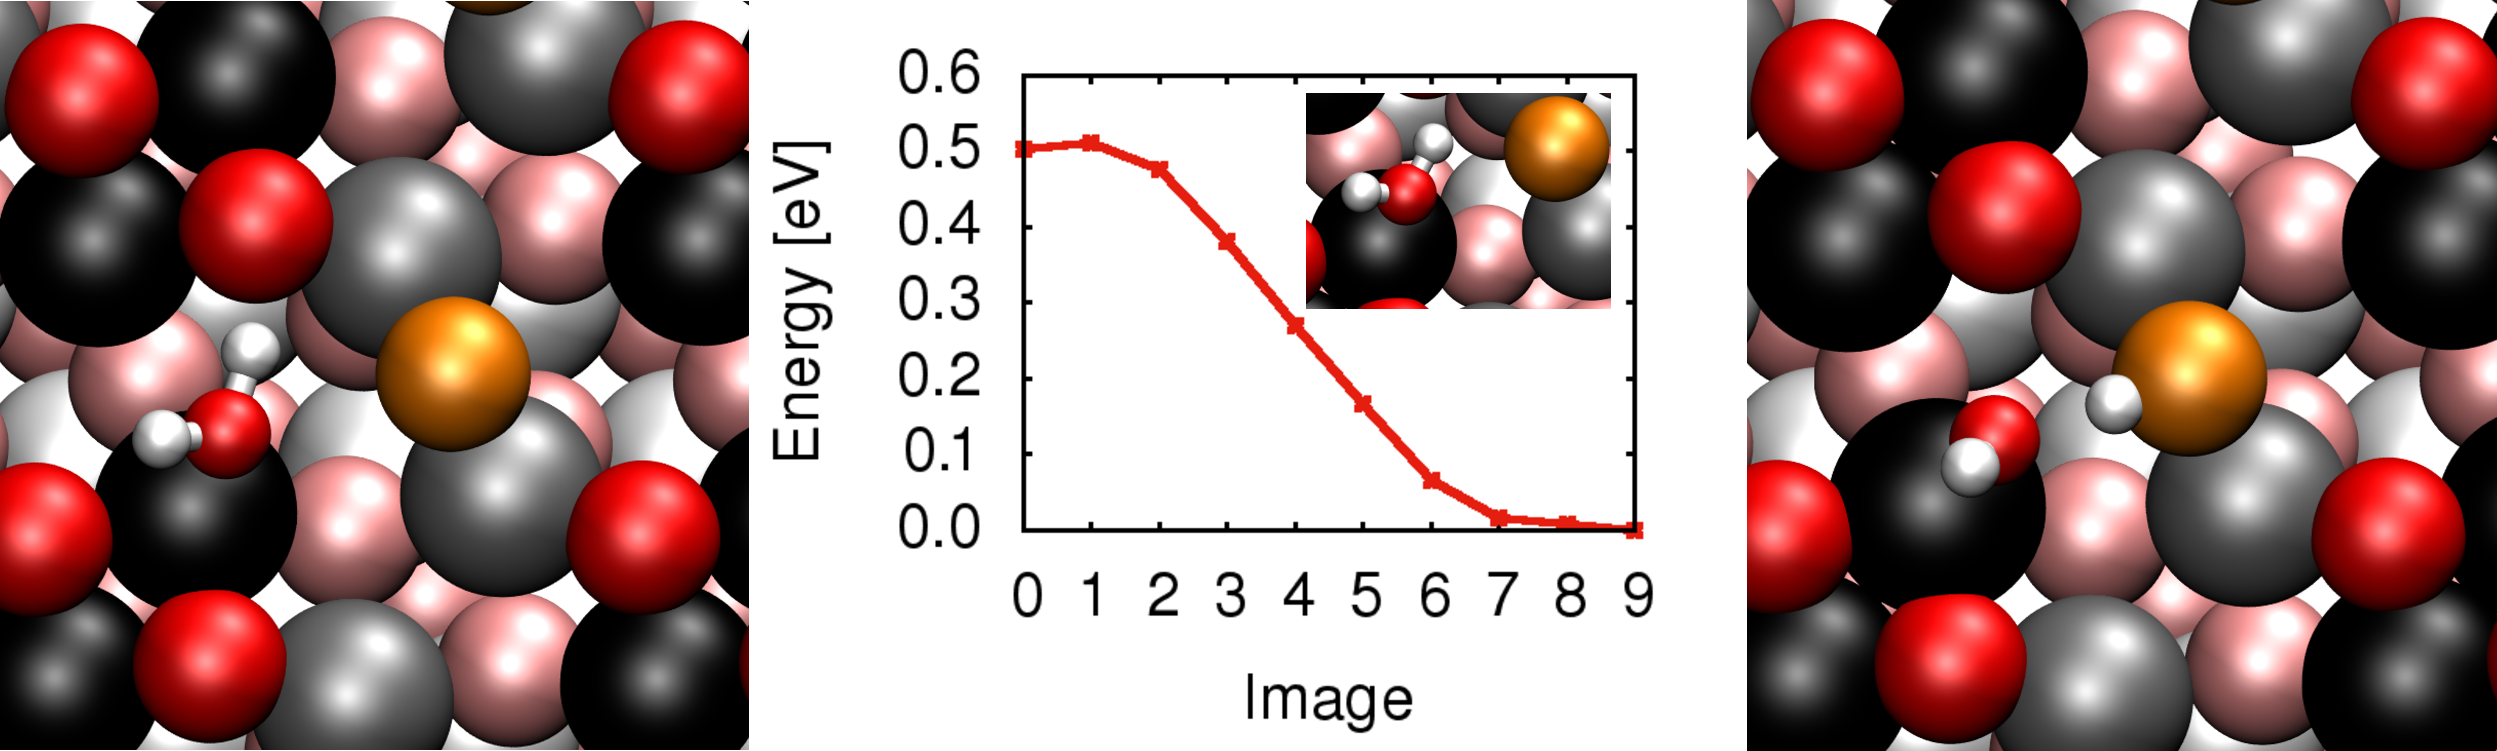
\includegraphics[width=0.7\textwidth]{figures/11-20/Diss_Cb-Cb2.pdf}}
         \quad
\subfigure[D-b: CUSb $\rightarrow$CUSb||O-$\mu_3$]{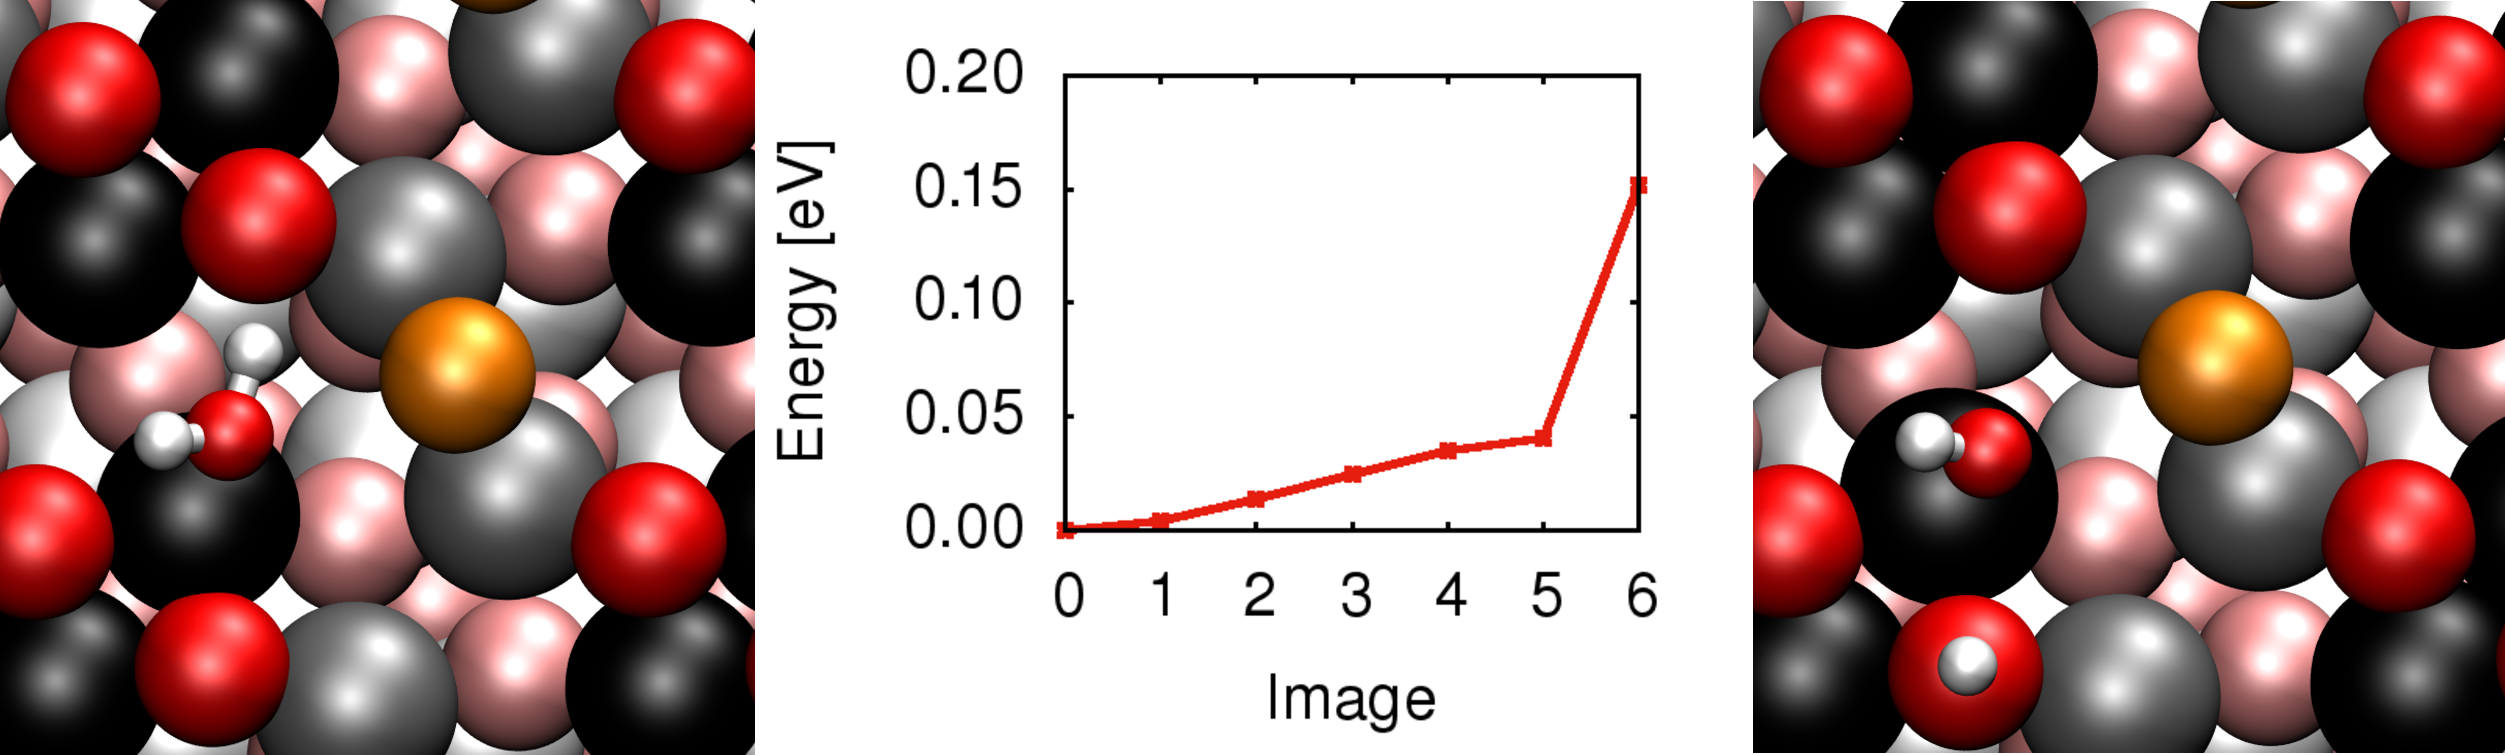
\includegraphics[width=.7\textwidth]{figures/11-20/Diss_Cb-Cb3.pdf}}
 \quad
\subfigure[Df-OH-a: CUSb||O-$\mu_2$ $\rightarrow$inter-CUSb||O-$\mu_2$]{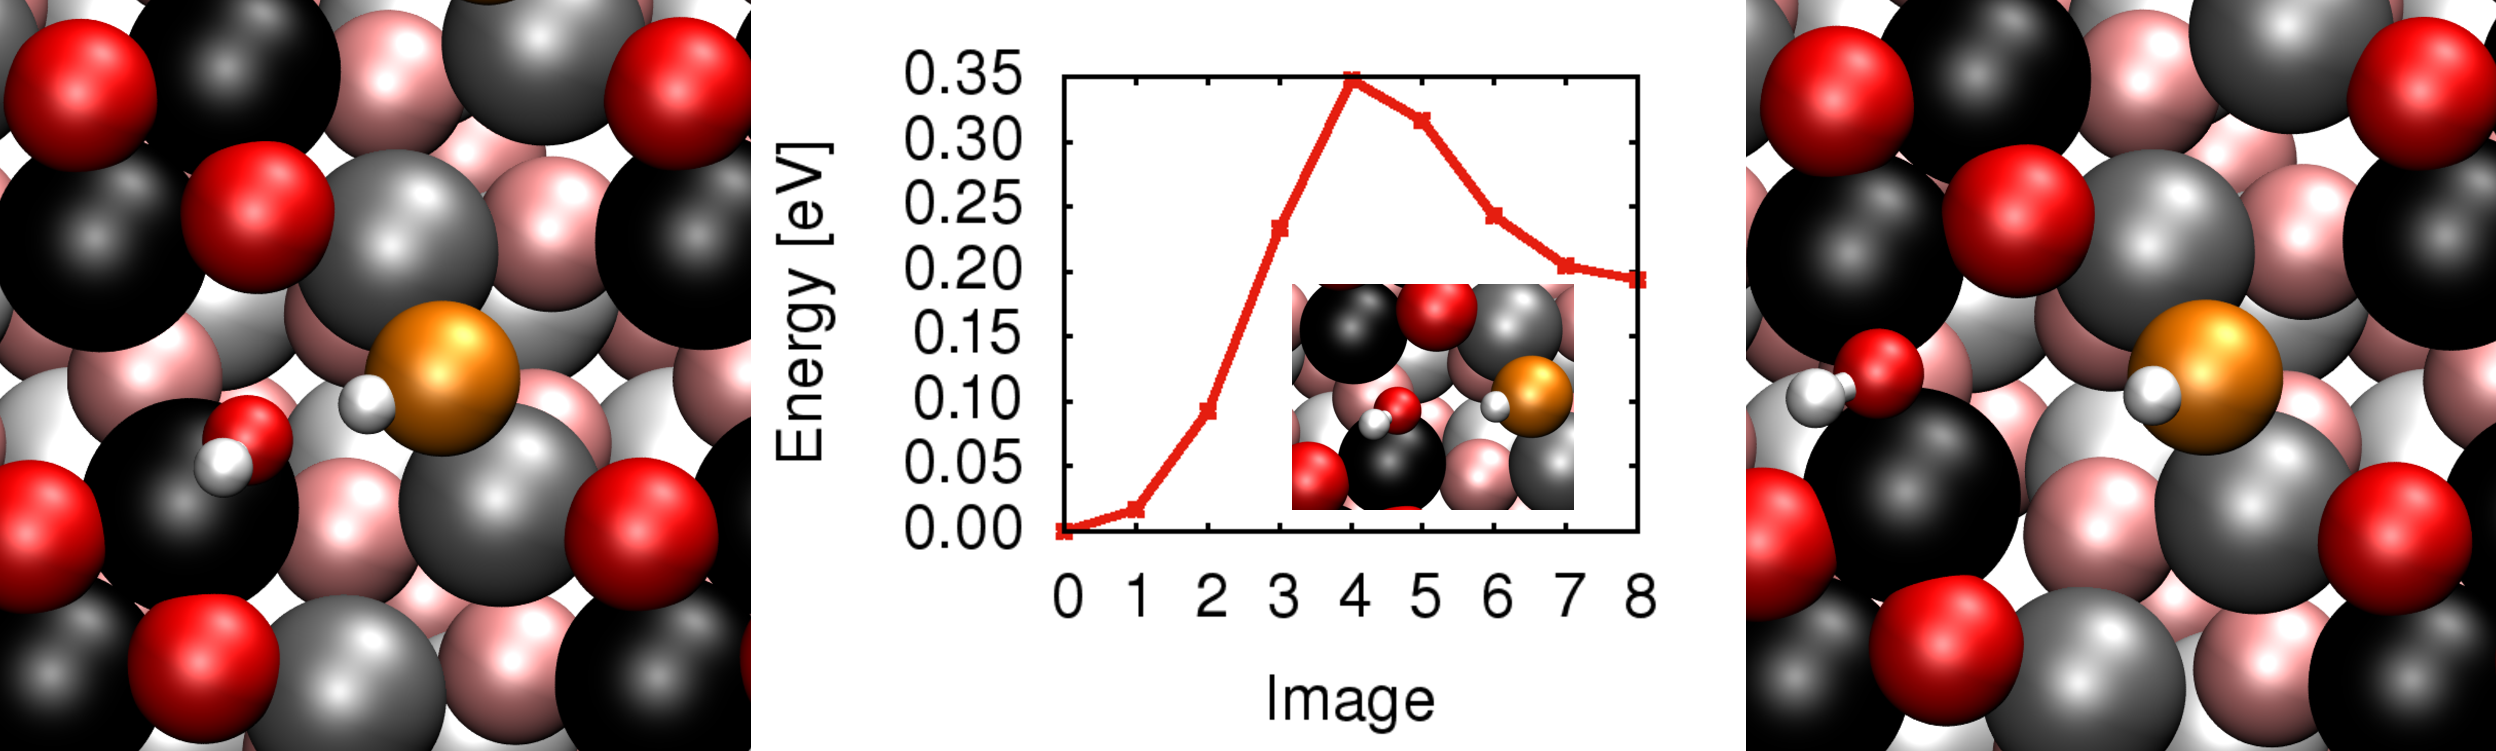
\includegraphics[width=.7\textwidth]{figures/11-20/Diff-OH_Cb2-iCb2.pdf}}
 \quad
\subfigure[Df-OH-b: CUSb||O-$\mu_2$ $\rightarrow$inter-CUSa||O-$\mu_2$]{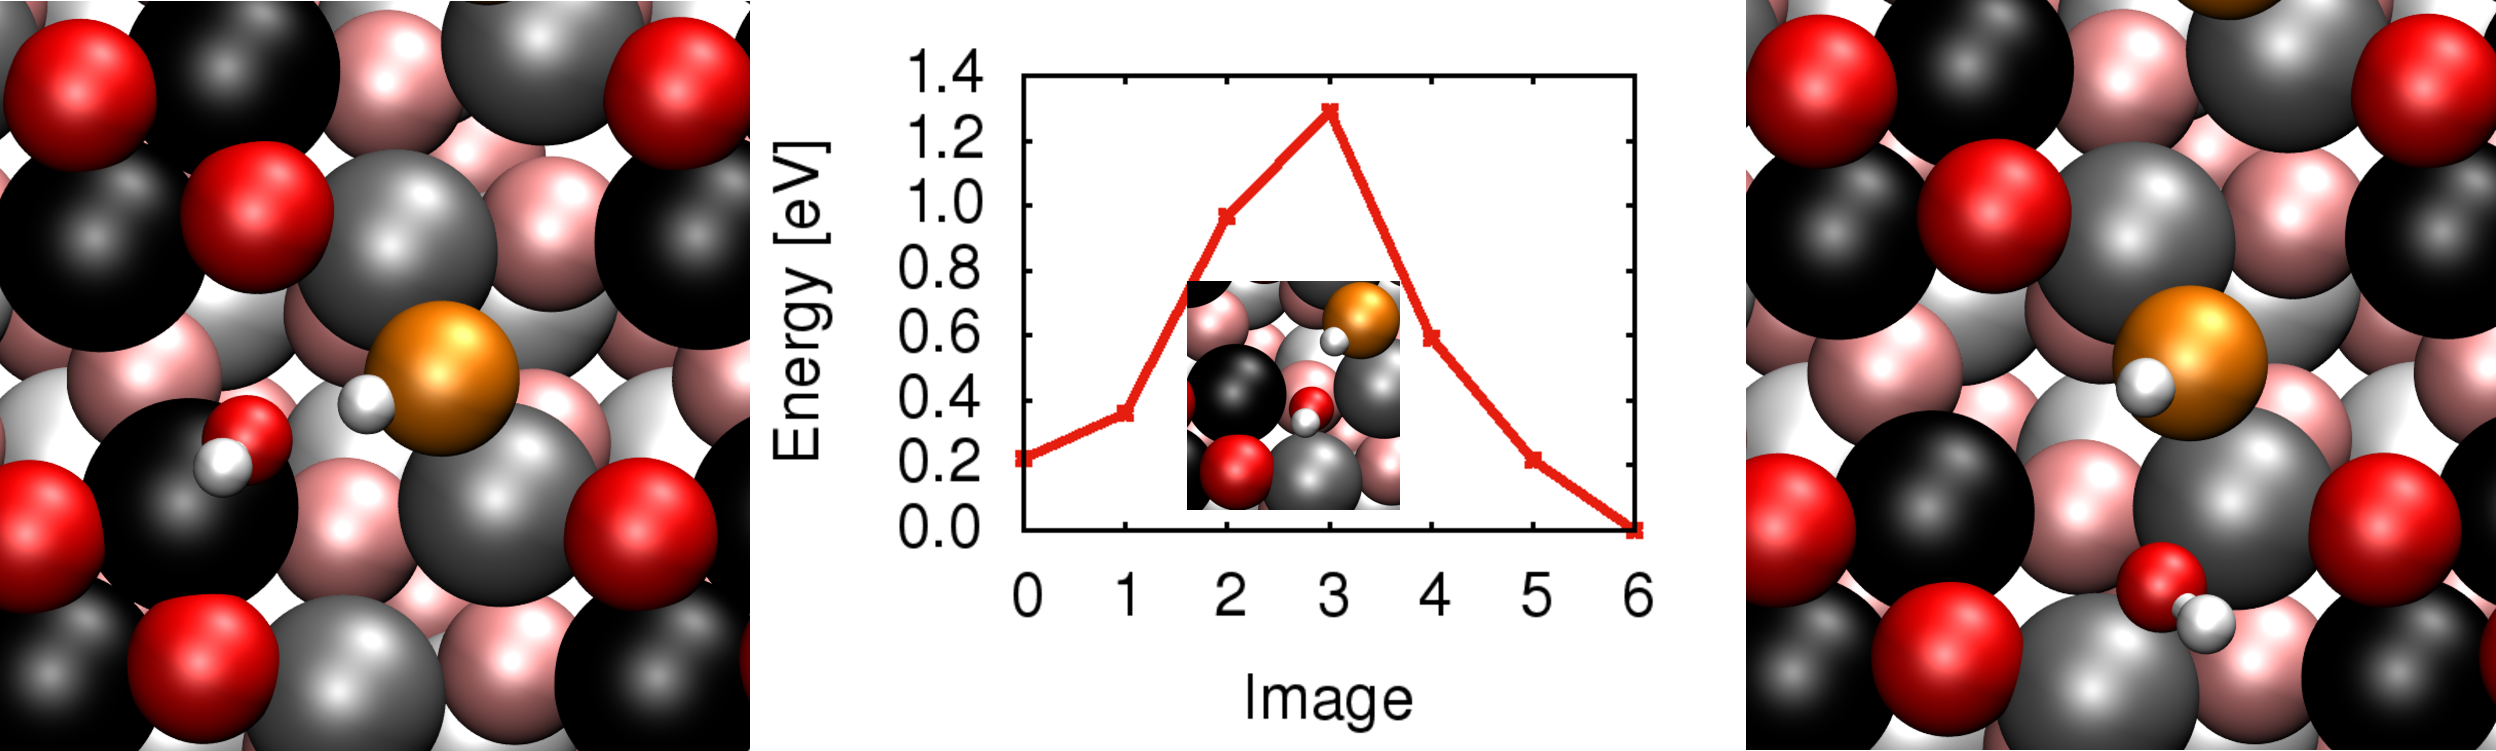
\includegraphics[width=.7\textwidth]{figures/11-20/Diff-OH_Cb2-iCa2.pdf}}
\caption{Minimum energy paths with transition states (inlay; if available), and both educt (left) and product (right) states for D-a, D-b, D-c, Df-OH-a and Df-OH-b reactions, respectively. The color code is as explained above.}
       \label{mep}
\end{figure*}
\begin{figure*} [!ht]
\centering
\subfigure[Df-H-b: inter-CUSa||O-$\mu_2\rightarrow$inter-CUSa||O-$\mu_3^\prime$]{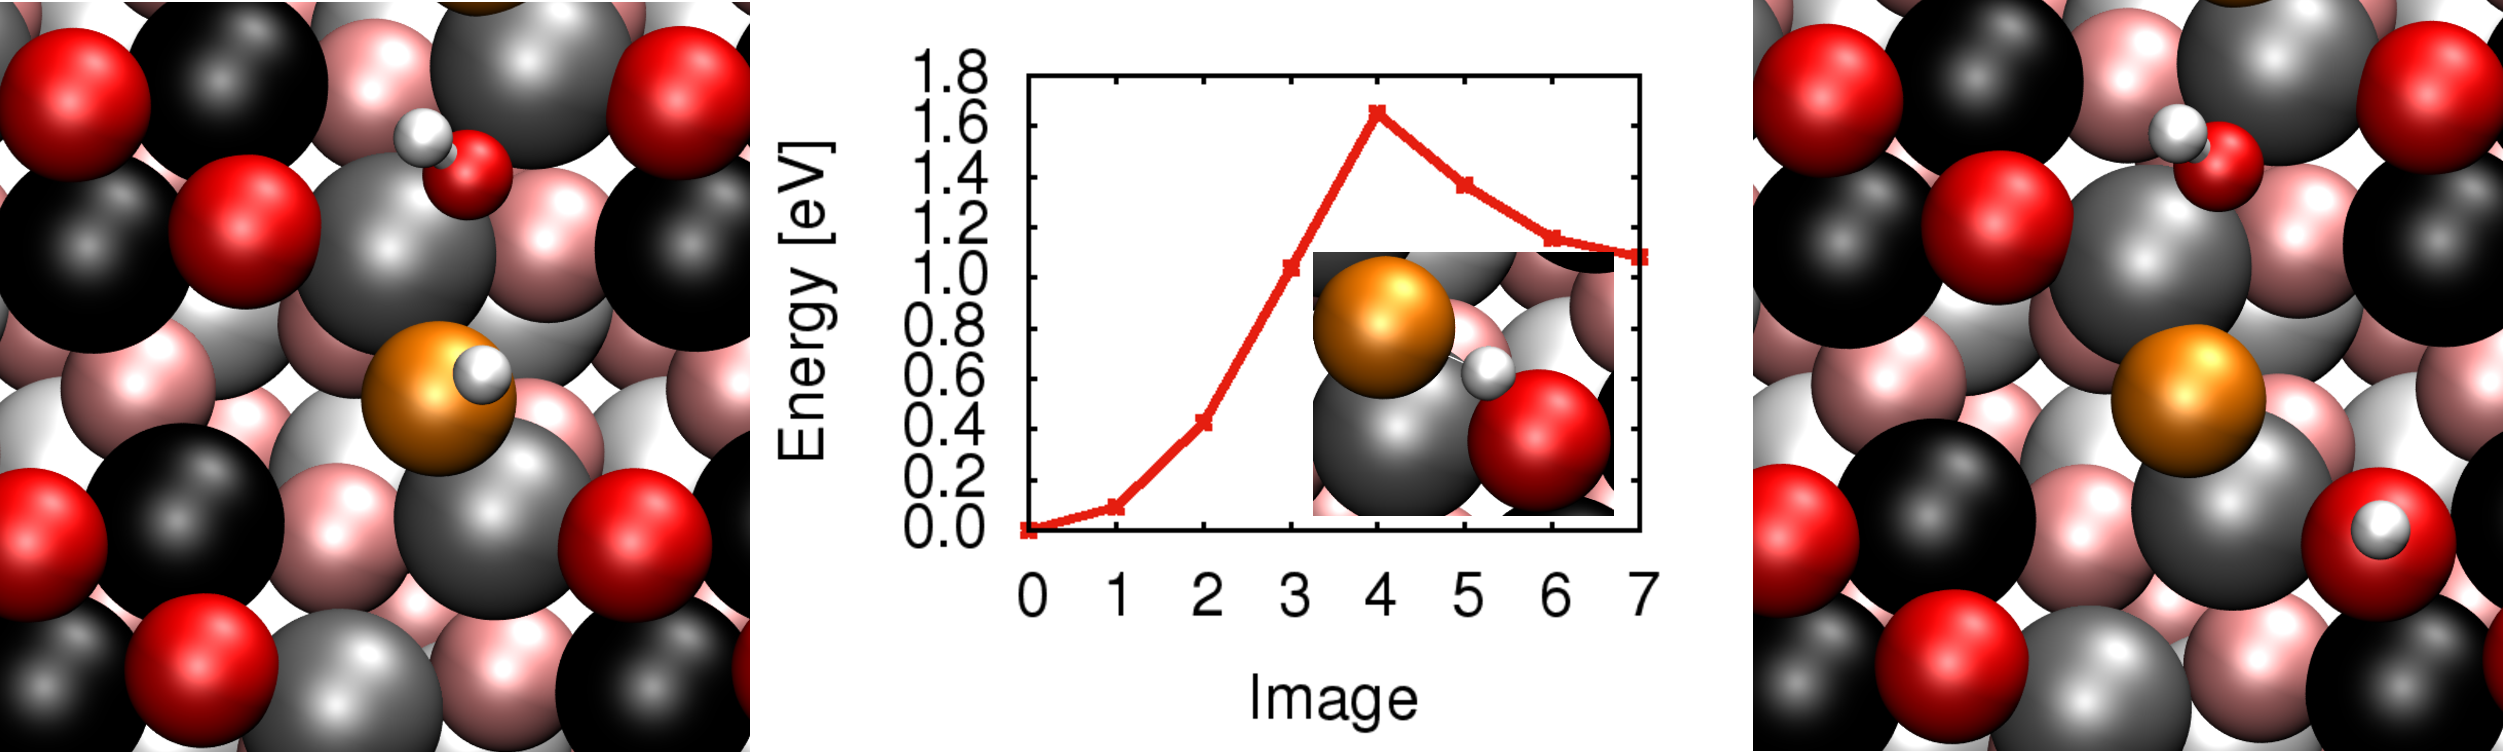
\includegraphics[width=.7\textwidth]{figures/11-20/Diff-H_iCa2-iCa3p.pdf}}
 \quad
 \subfigure[Df-H-c: inter-CUSb||O-$\mu_2^\prime\rightarrow$inter-CUSb||O-$\mu_3^{\prime\prime}$]{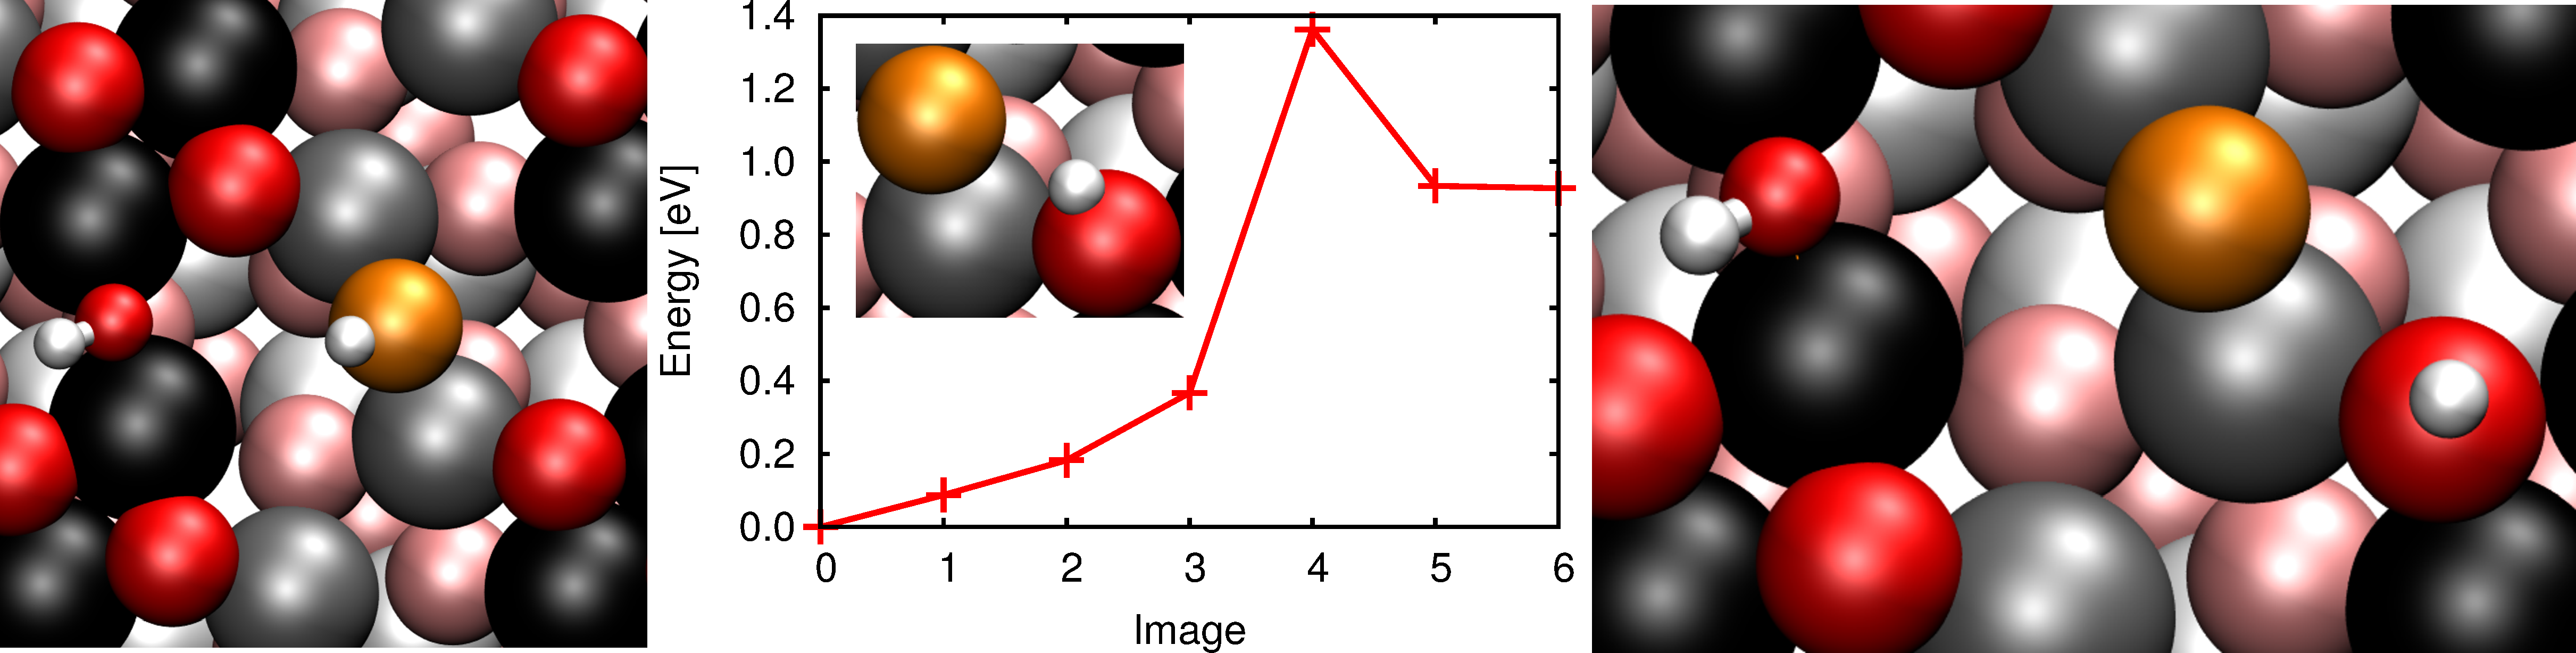
\includegraphics[width=.7\textwidth]{figures/11-20/Diff-H_iCb2p-iCb3pp.pdf}}
 \quad
\subfigure[Df-H-d: inter-CUSb||O-$\mu_3^{\prime\prime}$ $\rightarrow$inter-CUSb||O-$\mu_3^{\prime\prime\prime}$]{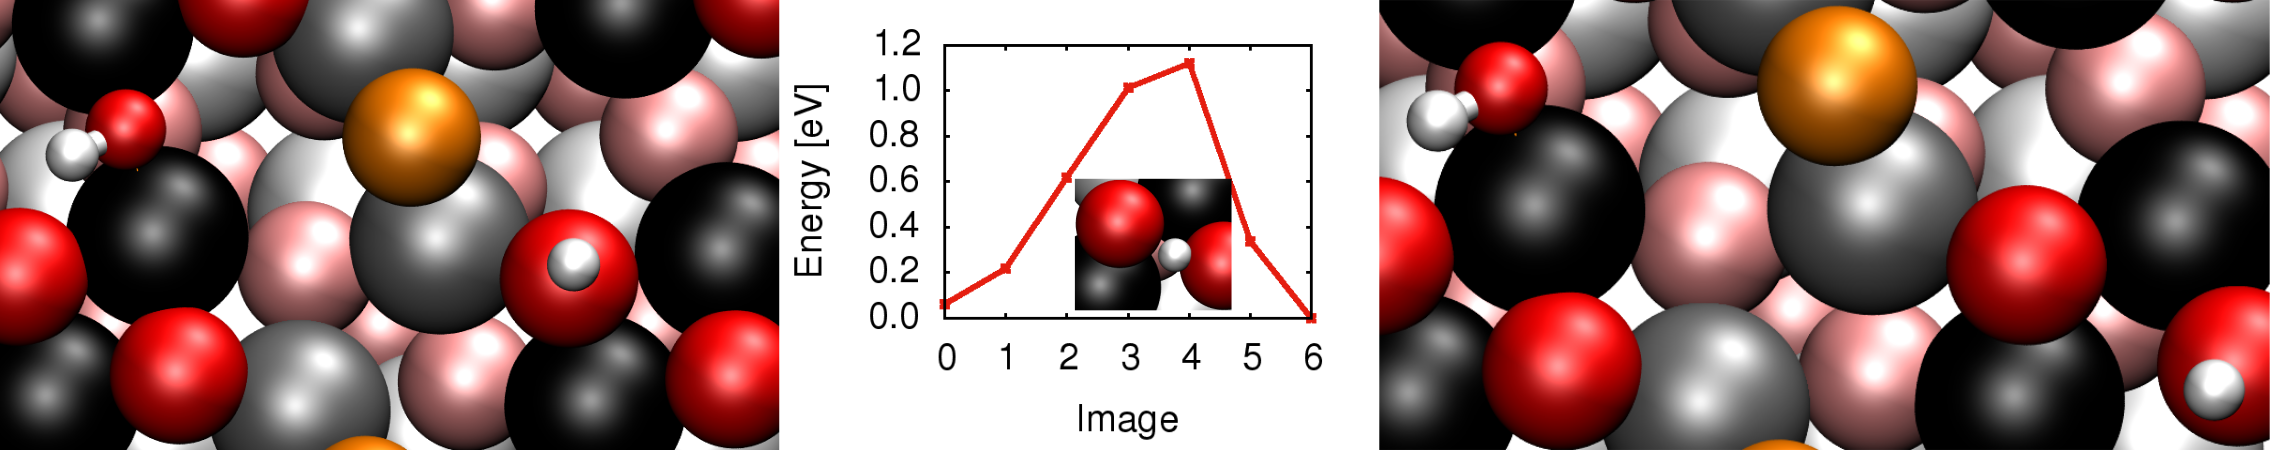
\includegraphics[width=.7\textwidth]{figures/11-20/Diff-H_iCb3pp-iCb3ppp.png}}
\caption{Minimum energy paths with transition states, and both educt and product states for Df-H-b - Df-H-d reactions. The color code is as explained above.}
       \label{mep2}
\end{figure*}

Rates for backreactions can also be calculated and the results are shown in Table \ref{tab:backreactions}.
\begin{table*}[ht]
  \centering
  \caption{Reaction rate constants for the backreactions in comparison with forward reactions (left). These rates can be calculated via detailed balance $\stackrel{\leftarrow}{k}  = \stackrel{\rightarrow}{k} \ e^{-\Delta G/k_B T}$. All values are given in s$^{-1}$ and at a temperature of $300\,$K.}
  \begin{tabular}{cl|cc|cc|c}
\small{Reaction Type} & \small{$k_\text{300 K}$(s$^{-1}$)} &  \small{$k_\text{300 K}$(s$^{-1}$)} \\
 &forward reaction &back reaction \\\hline
 \small{D-a}   & \small{5.76$\times 10^{12}$} &\small{1.17$\times 10^4$}\\
 \small{D-b}   & \small{n.f.} & \small{n.f.} \\
 \small{D-c}   & \small{n.f.} & \small{n.f.}  \\\hline
 \small{Df-OH-a} & \small{1.88 $\times  10^6$}&\small{9.86$\times 10^9$} \\
 \small{Df-OH-b}  & \small{2.41$\times 10^{-6}$}& \small{1.69$\times 10^{-8}$}\\\hline
 \small{Df-H-a} & \textit{no TST} &\textit{no TST} \\
 \small{Df-H-b}  & \small{4.90$\times 10^{-13}$} &\small{1.49$\times 10^5$} \\
 \small{Df-H-c} & \small{9.96$\times 10^{-10}$}& \small{9.95$\times 10^5$}\\
 \small{Df-H-d} & \small{1.05$\times 10^{-3}$} &\small{7.12$\times 10^{-5}$} \\
  \end{tabular}
  \label{tab:backreactions}
\end{table*}
\clearpage
\section{Vibrational Frequencies / Spectroscopic Properties}
A great source of knowledge about chemical systems is vibrational spectroscopy, so we were interested in frequencies of the systems, since the frequencies of these vibrations give us hints about the chemical environment as hydrogen bonds and other atoms nearby that bond to each other. These vibrational frequencies were calculated for the surface system adsorbed with OH and also with OD. Our experimental partners from FHI use deuterated water (D$_2$O) instead of H$_2$O because the chemical reactivity is the same but the spectroscopic properties are better with their applied Laser system. The experimental SFG spectra (Sum Frequency Generation) for the OD range of the low coverage regime for two different coverages are shown in Fig.~\ref{abb:exp-sfg}.
\begin{figure}[!ht]
 \centering
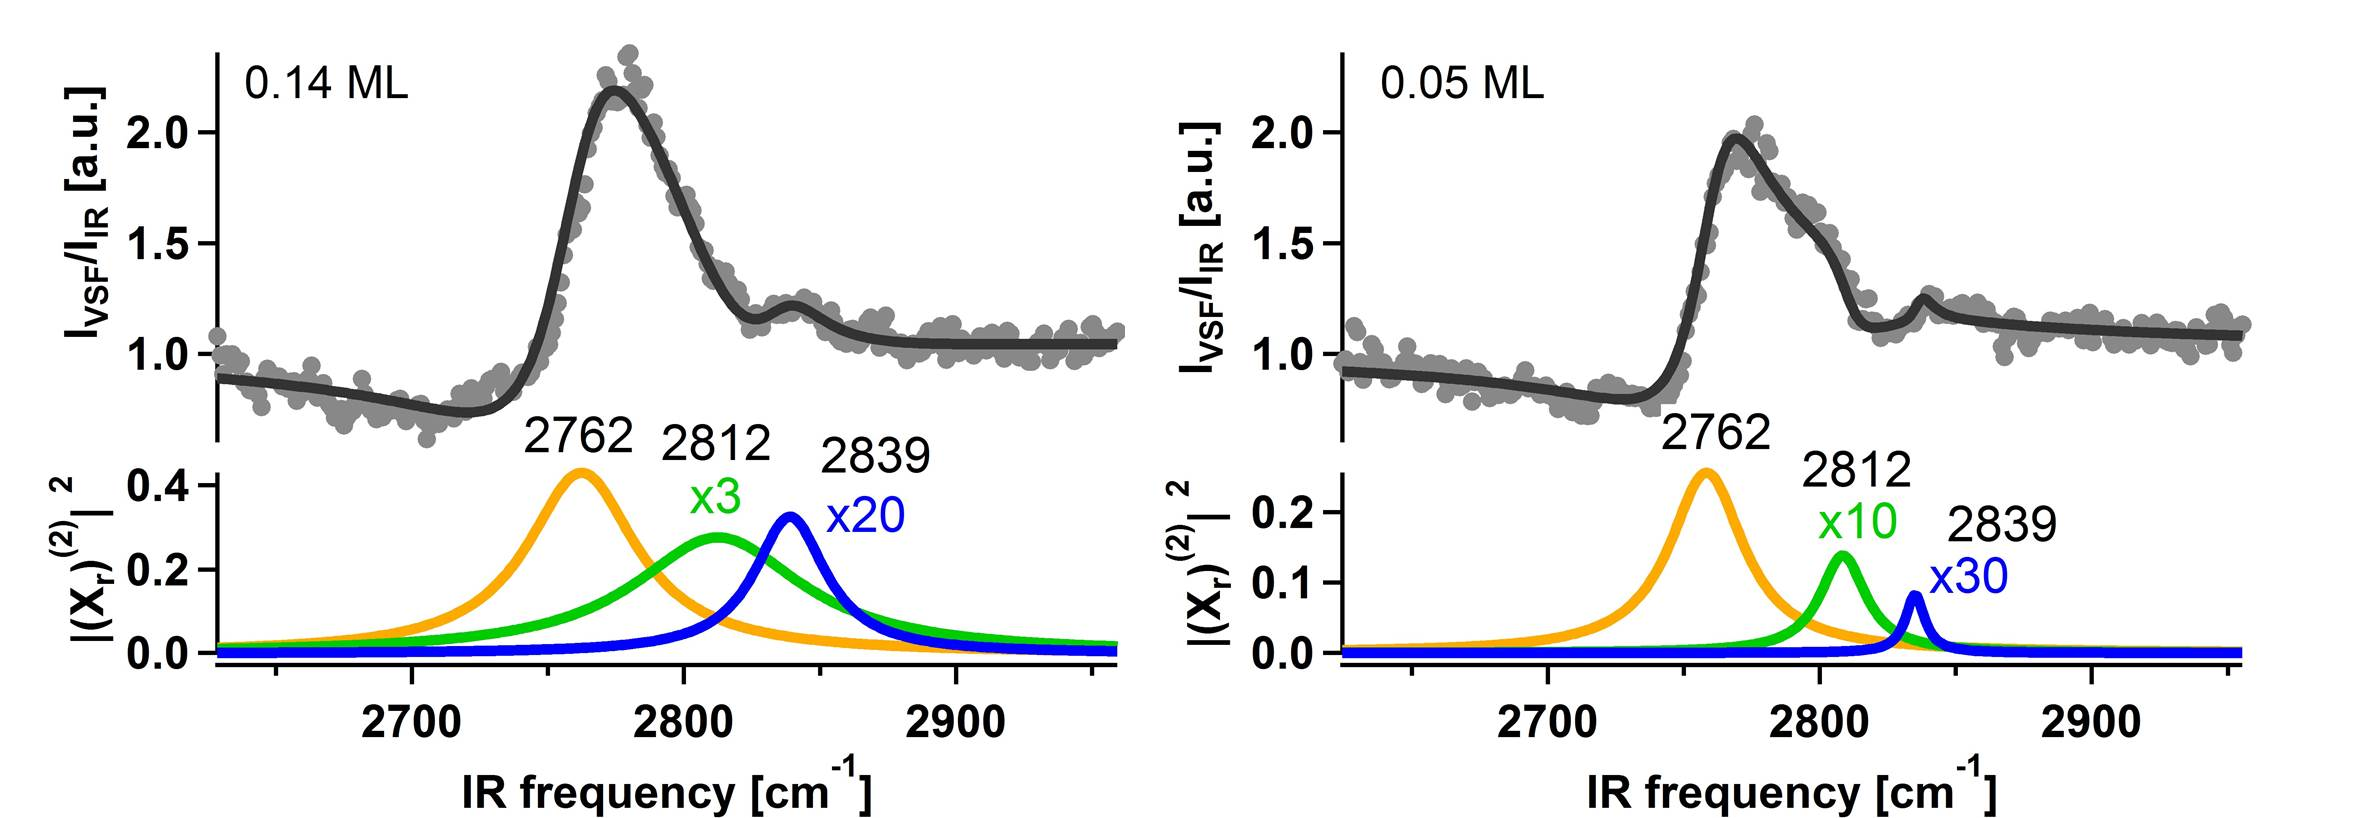
\includegraphics[width=0.9\textwidth]{figures/11-20/SFG_fit.jpg}
 \caption{Experimental SFG results for (11\=20) surface with 0.14ML (mono layer, left spectrum) and 0.05ML water coverage (right) including fit. The experiment was conducted by Yanhua Yue, FHI Berlin. Coverage only influences intensity of the peaks but not the peak position itself. The different coverages are achieved via different preparing temperatures of the sample.}
        \label{abb:exp-sfg}
 \end{figure}
Of course, the frequencies for a deuterated system are different from OH, but the different isotopes can be calculated easily within vasp, just by changing the mass.
\\
{\color{red} Better put this in theory part? In experiment the alumina single crystal was cleaned in ethanol and Milli-Q water and dried with N$_2$ before being installed in the ultra high vacuum chamber. It was then sputtered in Ar, and annealed to high temperatures in UHV and afterwards three times in oxygen at different temperatures. After this treatment, D$_2$O was brought onto the surface with a molecular beam source. For further details see cite{11-20paper} and the supporting information.}
\\
To calculate the modes in this work mainly two methods were applied: Normal mode analyses (see section \ref{nma}) and for some systems also power spectra from \textit{ab-initio} MD via velocity-velocity autocorrelation function (section \ref{vvacf}).
\\
We focus mainly on the position of the peaks rather than the intensities, because in the first place it is of greater interest what kind of vibrations gives which peak than the intensity of this peak. It is also still challenging to get the frequencies right before heading to intensities.
In the power spectra from MD calculations the intensities are implicitly received and for the normal mode analyses this work follows 2 different approaches, dipole corrections and Born effective charges.
\\
In subsection \ref{nma}, also modes for higher coverage systems are also examined.
\\
But not only the OH/OD frequencies are of interest, but also the lattice vibrations, and are covered in both subsections.

\subsection{Normal Mode Analysis}\label{nma}
\subsubsection{OD Vibrations}
The normal modes are within the harmonic approximation and depend on the mass and the spring constant of the bond. This ansatz is quite good for high frequency modes like OD stretch vibrations. We assumed that the OD stretching modes for the 3 most stable structures would contribute to the spectrum the most (see Table \ref{tab:freq_layers}).
\begin{table*}[th]
  \centering
 \caption{Comparison of the different slab sizes (normal modes): OD stretching modes for each of the most stable minima. In parantheses, the angle of the OD bonding vector to the surface normal ($\theta$ in \textdegree) is given. The left value reflects the adsorbed OD group and the right wavenumber the surface OD group, respectively.}
\vspace*{.2cm} 
 \begin{tabular}{l|cccc}
  Layers&inter-CUSa$\parallel$O-$\mu_2$ &CUSb$\parallel$O-$\mu_2$  &inter-CUSb$\parallel$O-$\mu_2$ \\\hline
  10 &2731 (44), 2694 (36) &2785 (26), 1711 (61) &2692 (41), 2689 (54) \\
  15 &2728 (44), 2695 (36) &2783 (24), 1812 (60) &2711 (34), 2656 (60) \\
  20 &2729 (44), 2694 (35) &2783 (24), 1838 (60) &2715 (34), 2665 (58) \\
  25 &2728 (44), 2696 (35) &2767 (59), 1750 (62) &2764 (29), 2724 (41) \\\hline
  exp. & \multicolumn{3}{c}{2839, 2812, 2762} \\
  \end{tabular} 
  \label{tab:freq_layers}
\end{table*}
Of course, all molecular and next neighbor dissociated structures from 10 to the 25 slab layer model were calculated, although as it was mentioned in section \ref{structure_search11-20} that the slab was already converged with 10 layers concerning OD stretch frequencies. Following this approach we expect 6 modes, for each of the three an OD$_{surf}$ and an OD$_{ads}$. In all cases the relationship between the two individual modes for each considered structure is portrayed by $\tilde{\nu}$(OD$_{ads}$)>$\tilde{\nu}$(OD$_{surf}$). This can be explained with the different reduced mass for both vibrations: The OD$_{surf}$ oscillator has a slightly larger reduced mass since the deuterium is bound directly to the surface, whereas the adsorbed OD group can act more as a quasi-free OD group {\color{red} cite{kirsch2014}}. All these vibrations are clearly localized on one of the OD groups, which suggests that the normal modes ansatz is reasonable.
\\
To consider the probability of observing these species, we calculated their respective Boltzmann weights $P_i$:
\begin{equation}\label{boltzmann-weight}
 P_i=e^{-G_i/(k_BT)}.
\end{equation}
With this analysis it is possible to show the relative population for different temperatures, see Table \ref{tab:boltzmann-pop}. In the whole temperature range relevant for the experiments, it is shown that the population of the species inter-CUSa$\parallel$O-$\mu_2$ clearly dominates and that the population of inter-CUSb$\parallel$O-$\mu_2$ is very low, compared to the others.
\begin{table*}[th]
  \centering
 \caption{Boltzmann population relative to the most stable inter-CUSa$\parallel$O$\mu_2$, calculated according to eq.~\ref{boltzmann-weight}.}
\vspace*{.2cm} 
 \begin{tabular}{l|ccc}
  & P$_{130K}$ & P$_{300K}$ & P$_{400K}$\\\hline
  inter-CUSa$\parallel$O-$\mu_2$ &1 &1 &1 \\
  CUSb$\parallel$O-$\mu_2$ & 1.4$\times 10^{-6}$& 6.1$\times 10^{-3}$& 3.2$\times 10^{-2}$\\
  inter-CUSb$\parallel$O-$\mu_2$ & 1.0$\times 10^{-15}$ & 1.2$\times 10^{-6}$ & 6.6$\times 10^{-5}$\\
  \end{tabular} 
  \label{tab:boltzmann-pop}
\end{table*}
\\
With the results for the frequencies of the three most stable structures (here the inter-CUSb$\parallel$O-$\mu_2$ results are shown for completeness), one can see, that for all slab sizes, there are 4 relevant modes. One of them is noticeable lower in energy that is due to hydrogen bonding. Also the angle of the bonding vector with respect to the surface normal is very high (i.e. the bond is more in plain, values shown Tab.~\ref{tab:freq_layers}, schematic representation in Tab.~\ref{tab:rel_modes}) so that the expected intensity in experiment is remarkably lower and may be not visible in experiment because of the angle dependence of the intensity in VSF. 
\\
With this in mind, we are able to predict 3 peaks, which fits well to the experimental results (see Fig.~\ref{abb:exp-sfg}). Comparing these results in absolute numbers is not very convincing as before in the literature, but relative numbers are in good agreement (see results for experiment and all different sized layer slabs in Table \ref{tab:rel_modes}).
\begin{table*}[!h]
\begin{center}
\caption{Frequency differences $\Delta \tilde{\nu}$ are given in [cm$^{-1}$]. $\Delta \tilde{\nu}_1$ depicts the difference between the surface OD group of the inter-CUSa$\parallel$O-$\mu_2$ species and the respective surface OD group on O-$\mu_2$ and  $\Delta \tilde{\nu}_2$ is the difference between the same surface OD group and the adsorbed OD group on CUSb from CUSb$\parallel$O-$\mu_2$. In the right half a sketch of the angle $\theta$ between the OD bond and the surface normal is shown.}
%{Vibrational frequencies and VSF resonances as observed at $300$ and $400\,$K, all in cm$^{-1}$. Also listed are frequency differences $\Delta {\tilde{\nu}}$, relative to the lowest frequency. An assignment of the modes is given. The O-D tilting angles $\theta$ are listed once more for clarity.}
\begin{tabular}{cccc}
layers & $\Delta \tilde{\nu}_1$ &  $\Delta \tilde{\nu}_2$&\multirow{6}{1pt}{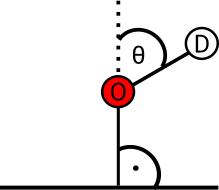
\includegraphics[width=2cm]{figures/11-20/ODangle.png}}\\\hline
10  &37 &91 & \\
15  &33 &88 & \\
20  &35 &89 & \\
25  &32 &71 & \\\hline
exp.&50 &77 & \\
% \begin{tabular}{cl|c|cc|cc}
% \multicolumn{2}{c|}{assignment}   & $\theta / ^{\circ}$ & $\tilde{\nu} _\mathrm{cal}$  & $\Delta{\tilde{\nu}}_{\mathrm{cal}}$ & $\tilde{\nu}_\mathrm{exp}$ & $ \Delta{\tilde{\nu}}_{\mathrm{exp}}$ \\\hline
% \multirow{2}{*}{inter-CUSa||O-$\mu_2$} & D(O-$\mu_2$) & 36 &  2694 &    & 2762 &  \\
% & OD(inter-CUSa)  & 44 & 2731 & 37 & 2812 & 50  \\\hline
% CUSb||O-$\mu_2$ & OD(CUSb)       & 26 & 2785 & 91 & 2839 & 77 \\
  \end{tabular}
\label{tab:rel_modes}
\end{center}
\end{table*}
\\
Two problems of this approach are, that we neglect anharmonicities, that are especially important for hydrogen bonded vibrations and also the absence of neighbor effects, that can be solved by computing higher coverage systems.
\\
The influence of higher coverage was examined for some test systems already presented in section \ref{structure_search11-20}. The coverage differs from 2D$_2$O molecules per super cell to 4 and 12 water molecules (equals 1ML). {\color{red} Here the frequencies of the OD stretching modes are affected due to the neighbor effects, for some structures more and for other less (e.g. the system with 2inter-CUSa$\parallel$O-$\mu_2$).
compare modes of low coverage limit to spetra with higher coverage, ask Lu for more data of higher coverage.
}

{\color{red} The simulation of intensities was done both with dipole corrections and Born effective charges and is shown here as a comparison. {\textit{show only high frequency part, comparing BEC and dipole, for the most stable configurations. These are only IR intensities in both cases, that can not be set equal to SFG intensities but can be a first hint.}}
}
\\
{\color{blue} Frequencies for the low coverage limit were also calculated using the crystal code, that enables calculations with atomic centered bases and makes it possible to treat a real 2-D system without the need to calculate the repetition of the slab in z-direction, see also section \ref{crystal_calc}. With this code it is also possible to calculate hybrid functionals, here B3LYP easily. For both PBE and B3LYP, geometries of the most stable states were optimized and from those geometries normal modes were calculated. Also anharmonicities for OH/OD bonds could be calculated, results in comparison with vasp results are shown in Table \ref{tab:freqs11-20crystal}. First of all, PBE results from both programs do not differ largely. anharmonicities decrease the wavenumbers and lead to worse agreement to experiment and to vasp calculations. Data from B3LYP calculations show great agreement with experiment, although here, anharmonic corrections make the agreement worse, too. One has to mention, that here influence of the basis set is strong and larger basis sets were not feasible due to high computational costs.
 \begin{table}[!h]
  \centering
   \caption{Stretch wavenumbers for both of the OD groups at the (11\=20) surface for the 3 most stable species, calculated with atom centered basis functions with the program crystal. Frequencies were calculated at the B3LYP and PBE level of theory, optimized with the respective method. The used basis set was pob\_TZVP. The VASP results were obtained with a plane wave basis and PBD+D2 corrections.}
  \begin{tabular}{ccc|cc|c}
   & \multicolumn{2}{c}{PBE} & \multicolumn{2}{c}{B3LYP} &VASP result\\
  stretch & $\tilde{\nu}$ [cm$^{-1}$] &$\tilde{\nu}$+anharm [cm$^{-1}$] &$\tilde{\nu}$ [cm$^{-1}$] & $\tilde{\nu}$+anharm [cm$^{-1}$]&$\tilde{\nu}$ [cm$^{-1}$]\\\hline
  iCa2: OD$_{\textrm{surf}}$ &2682 &2599 &2773 &2695 & 2694\\
  iCa2: OD$_{\textrm{ads}}$  &2728 &2644 &2811 &2729 & 2731\\
  Cb2: OD$_{\textrm{surf}}$  &1658 &1310 &2019 &1722 & 1711\\
  Cb2: OD$_{\textrm{ads}}$   &2769 &2687 &2843 &2765 & 2785\\
  iCb2: OD$_{\textrm{surf}}$ &2657 &2595 &2778 &2694 & 2689\\
  iCb2: OD$_{\textrm{ads}}$  &2688 &2569 &2777 &2689 & 2692\\
  \end{tabular}
  \label{tab:freqs11-20crystal}
  \end{table}
}
\subsubsection{Lattice Vibrations}\label{phonons}
For the phonons as a first test the same normal modes analyses were checked to get a first impression into how the spectra can look like. But for a better description we need to consider more layers of the bulk in order to get more reliable results. From an experimental point of view it is suggested that SFG spectra can give insight into {\color{red} x} layers of the bulk {\color{red} ask Lu!}. Therefore we did calculations for the most stable adsorption geometries for more layered systems, going up to 6*5=30 layers (with 5 being the number of layers in the unit cell in z direction), both for the clean surface and for the adsorbate covered surface, here we used again optimized geometries of the most stable structures. These results are also shown with intensities calculated from dipole corrected normal mode analyses. The additional geometries with more layers do not differ strongly from the 10 layer ones that were presented in section \ref{structure_search11-20}.
\\
{\color{red} Table with no. of layers and adsorption energies? Put it to section \ref{structure_search11-20}? Probably better do do it there!}
{\color{red} compare clean surface for different sizes, iCa2, Cb2 and iCb2 for all slab sizes. Normal modes may not be a perfect description of these deeply delocalized vibrations.. intensities for lattice vibrations from BEC and dip..}
\subsection{Velocity-Velocity Autocorrelation Function}\label{vvacf}
Extract vel vel autocorrelation function from MD at $300\,$K (and also $400\,$K?) from most stable structures (inter-CUSa||O-$\mu_2$, CUSb||O-$\mu_2$ and inter-CUSb||O-$\mu_2$), with Fourier transformation converted to VDOS spectrum. It also is possible to separate modes from water layers from bulk phonons. Not really important if you don't use hydroxylated surface with a higher water coverage? So for Giacomo's system it makes sense, but here it is unnecessary.

{\color{red} totally different ansatz, no freq analysis, no harmonic approximation, but ab-initio MD trajectories at 300K, starting from optimized minimum structures. trajectory duration of 1-a few ps. calculating vac, fourier transform gives power spectra, no real IR, but still one can relate to intensities. results for trajectories.}
\section{Desorption Process}
Not only the reactions at the surface are of interest but also the process of adsorption and desorption were studied. The experimentalist's method to do so is TPD (thermal desorption spectroscopy). It is possible to measure the bond strength of the adsorbates, depending on the temperature they can be found in the corresponding spectrum. The sample was flashed to $400\,$K to get rid of impurities. The results showed two peaks, one beneath $400\,$K and one above. This peak beneath $400\,$K hould not be visible, since the sample was heated to that temperature and all adsorbates that are released beneath this temperature should not be there any more. The only plausible explanation to this is, that there are reactions, that fill this species up and so the desorption can still be from this species.
\\
To interpret these results, one has to think of a possible reaction scheme from the most stable adsorption sites via the molecular state leading to the gas phase molecule.
\\
Here the most stable inter-CUSa$\parallel$O-$\mu_2$, CUSb$\parallel$O-$\mu_2$ and inter-CUSb$\parallel$O-$\mu_2$ and their reactions


\textit{not sure if this is worth a whole chapter..}
\\
calculation with NEB was not done, instead geometry optimization for a water molecule above 3 interesting points on the potential energy surface (above inter-CUSa, CUSb and inter-CUSb).
\begin{verbatim}
  /und/sophia/bigger-cell_newcrystalcut/2x2cell/2layers/gasphase-physisorbed
\end{verbatim}

It was also tried to study the adsorption/desorption process (not with NEB), since there was no minimum structure in the gas phase nor physisorbed state. But from a single water molecule above the surface, geometry optimizations were done. Three structures were tested above inter-CUSa, CUSb and inter-CUSb. The energy profile is smooth from any tested point on the potential energy surface above the alumina surface towards the adsorbed water system without showing a barrier but indeed both showing an intermittend molecularly adsorbed structure.
\\
As mentioned before the experimentalists measure TPD in order to understand the adsorption strength and possible exchange reactions. We tried to simulate the desorption process using the following scheme: take the water in the gas phase + the clean surface as the standard. In the thermal equilibrium, the water should be equally distributed to Boltzman's distribution in the most stable structures. From this situation the water can recombine to the molecularly adsorbed water. The recombined water then can desorb to the gas phase. Since the spectrum is measured in ultra high vacuum it can be assumed that all the water that has left the surface will not return to the system, because it is dragged out of the equilibrium by the vacuum pumps.
Applying the reaction rates of the corresponding reactions in a kinetic Monte Carlo approach leads to 
{\color{red} Redo these calculations? I don't think that this is worth the effort..}.

{\color{green} does it make sense to bring this cause there is no good agreement between our theory and the experimental findings..? The NEB didn't lead to anything since there is no minimum (just try a NEB??), optimization doesn't show any kind of barrier and just modelling the desorption from the rates is not good enough, sonce the rate for Cb2-Cb is too small to }
%%%%%%%%%%%%%%%%%%%%%%%%%%%%%%%%%%%%%%%%%%%%%%%%%%%%%%%%%%%%%%%%%%%%%%%%%%%%%%%%%%%%%%%%%%%%%%%%%%%%%%%%%%%%%%%%%%%%%%%%%%%%%%%%%%%%%%%%%%%%%%%%%%%%%%%%%%%%%%%%%%%%%%%%%%%%%%%%%%%%%%%%%%%%%%%%%%%%%%%%%%%%%%%%%%%%%
%%%%%%%%%%%%%%%%%%%%%%%%%%%%%%%%%%%%%%%%%%%%%%%%%%%%%%%%%%%%%%%%%%%%%%%%%%%%%%%%%%%%%%%%%%%%%%%%%%%%%%%%%%%%%%%%%%%%%%%%%%%%%%%%%%%%%%%%%%%%%%%%%%%%%%%%%%%%%%%%%%%%%%%%%%%%%%%%%%%%%%%%%%%%%%%%%%%%%%%%%%%%%%%%%%%%%

\chapter{Water on $\upalpha$-Al$_2$O$_3$(0001)}
The (0001) surface is the most stable surface site of alumina under UHV conditions, and was subject of several studies so far. Both experimental and theoretical studies discovered lots of characteristics and specialties of this crystal cut. In our workgroup previous work was done concerning the stability of low limit water coverage and their vibrational spectroscopic behaviour, reaction pathways between these stable minima, but also studying higher water coverages and hydroxylated surface systems. In this work, the focus lies more on two topics:
\\
(i) understanding the processes of a water molecule (D$_2$O) being shot at the surface with a molecular beam source with the help of \textit{ab-initio} Molecular Dynamics and
\\
(ii) the improvement of reaction rates with different methods beyond GGA functionals (as PBE).
\\
First, the surface and the most stable adsorption patterns are introduced (section \ref{sec_0001surf}), followed by the results for the molecular beam scattering (section \ref{sec_0001AIMD}) and last the improvements for the reaction rates (see section \ref{sec_rates}).
	
\section{Surface Model and Static Calculations}\label{sec_0001surf}
The most stable surface cut is a stochiometric, Al terminated one, and in contrast to the (11\=20) surface there is only one type of Al-CUS atom, which is a reactive Lewis-acid site. Also, all oxygen atoms are 3-fold coordinated, that leads to a topography that is not as complex as for the higher indexed surfaces. We applied here a $2\times 2$ supercell with vectors that were optimized from the bulk structure vectors (previous work of J. Wirth). The surface slab consists of 9 atomic layers, that is three repeating units in z direction of the type Al-O$_3$-Al..., with the top 5 layers being allowed to relax during optimization and AIMD and the lowest 4 layers being fixed to bulk values, see Fig.~\ref{abb:surf_0001}. The unit cell vectors in there are equal to $\uline{a}=\uline{b}=9.66\,$\AA  ~and a $60$\textdegree ~angle between them. The $\uline{c}$-vector of the slab model is $31.4\,$\AA~ long, hence the vacuum gap between two slabs in this direction is $26.4\,$\AA.
\\
The stability, vibrations and reactivity of one water  molecule per $2\times 2$ supercell were already studied by Dr. Jonas Wirth. As it was published in ref{jonas0001}, there is one molecular minimum on top of a CUS atom and 3 dissociated states (see figure \ref{abb:0001_ads}): the next neighboring 1-2 dissociated state, the 1-4 dissociated structure with the Hydrogen atom being one position further and the 1-4$^\prime$ that is the configuration with the greatest distance that is possible for this slab size. From these, the 1-2 dissociated species is the most stable one and the 1-4$^\prime$ is the least stable one. For the stability of the molecular and the 1-4 dissociated species, the situation is more controversial in the literature. In our periodic DFT studies with VASP, it lies between the previously mentioned ones, depending on the exact method employed, for PBE+D2 the molecular adsorbed species is more stable than 1-4, for PW91+D2 the 1-4 dissociated is more stable, whereas PW91 without dispersion corrections gives the same adsorption energy for both species (the values for the adsorption energy are calculated analogously to the (11\=20) surface cut, see eq.~\ref{eq:Eads}).
Calculations with an atom centered basis instead of plane waves with the crystal code show, that for most basis sets the molecular species is more stable and for others, they are both equal in adsorption energy.
\\
Of course, there are reactions linking these minima, dissociation, OH- and H-diffusion were studied, as well as rotation of an OH group and molecular water diffusion from CUS to CUS. The latter two do not play a crucial role in this work, especially the CUS to CUS diffusion of molecular water is very improbable due to the slow reaction rate. Adsorption energies and reaction rates that are important for this work are shown in Table \ref{tab:0001_eads+rates}, these results were obtained by J. Wirth and were unpublished.
 \begin{table}[!h]
  \centering
   \caption{Adsorption energies for the stable minima (left part) and reaction rate constants $k$ in s$^{-1}$ at $300\,$K with corresponding barrier heigths $\Delta E^\ddagger$/$\Delta G^\ddagger_\textrm{300K}$ in eV for the processes connecting these minima (right part). Here the upper two line shows the reaction in the direction given in the name and the lower two line gives the back reaction's rates constants and barriers. All values were calculated with PBE including D2 dispersion corrections and are unpublished work of J. Wirth.}
  \begin{tabular}{cccc|ccccc}
   \multicolumn{4}{c}{E$_\textrm{ads}$ [eV]}&\multicolumn{5}{c}{k$_\textrm{300K}$ [s$^{-1}$]}\\
  mol &1-2 &1-4 &1-4$^\prime$  &diss-1-2            & diss-1-4            & diff-2-4         & diff-2-4$^\prime$ & diff-4-4$^\prime$\\
  -1.31 & -1.69 & -1.30 & -1.21&8.0$\times 10^{10}$  & 2.8$\times 10^{10}$ & 2.7$\times 10^1$  & 3.8$\times 10^1$  & 7.1$\times 10^5$ \\
   & & & &0.13/0.11 & 0.19/0.14& 0.82/0.68&0.81/0.67 &  0.61/0.41\\\hline
   & & &                       &2.3$\times 10^4$    & 2.7$\times 10^{10}$ & 9.1$\times 10^7$ & 3.1$\times 10^9$ & 1.7$\times 10^7$ \\
   & & & & 0.50/0.50 & 0.19/0.14 & 0.44/0.29 & 0.33/0.20 & 0.51/0.33\\
    \end{tabular}
  \label{tab:0001_eads+rates}
  \end{table}

The adsorption process itself was studied, by starting from the molecular minimum, gradually doing optimizations with greater O-surface distance and letting everything relax except for the c-coordinate of the water-oxygen atom. This calculations gives an energy profile for the adsorption/desorption but no barrier could be found (see Fig.~\ref{abb:0001_desorption}), so the underlying adsorption process is thought to be barrierless.
  \begin{figure}[!ht]
   \centering
   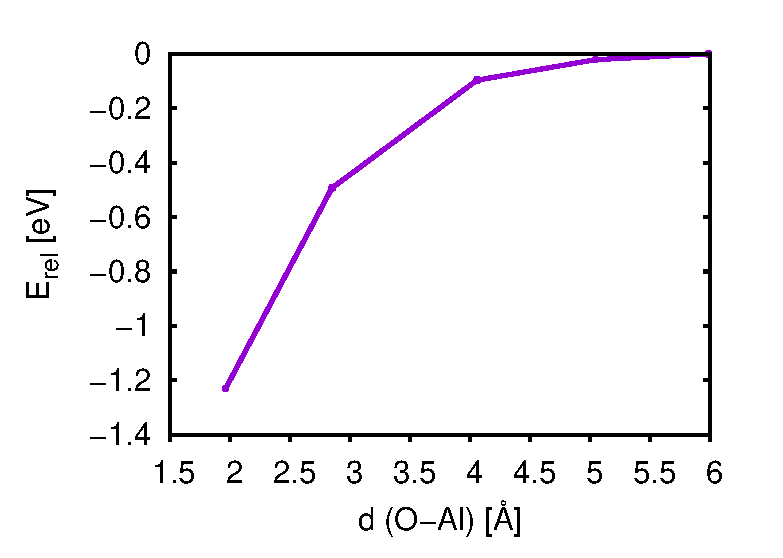
\includegraphics[width=0.45\textwidth]{figures/0001/mol_ads_barrier.eps}
   \caption{Energy profile of the adsorption process, relative to the energy of the system with a distance of $5.98\,$\AA. The d(O-Al) denotes the distance between the oxygen atom of the water and the Al-CUS where the water is/was adsorbed molecularly. %/und/sophia/0001_mol_ads_barrier/
   }
   \label{abb:0001_desorption}
  \end{figure}

  
  
\begin{figure}[!ht]
 \centering
\subfigure[(0001), top view]{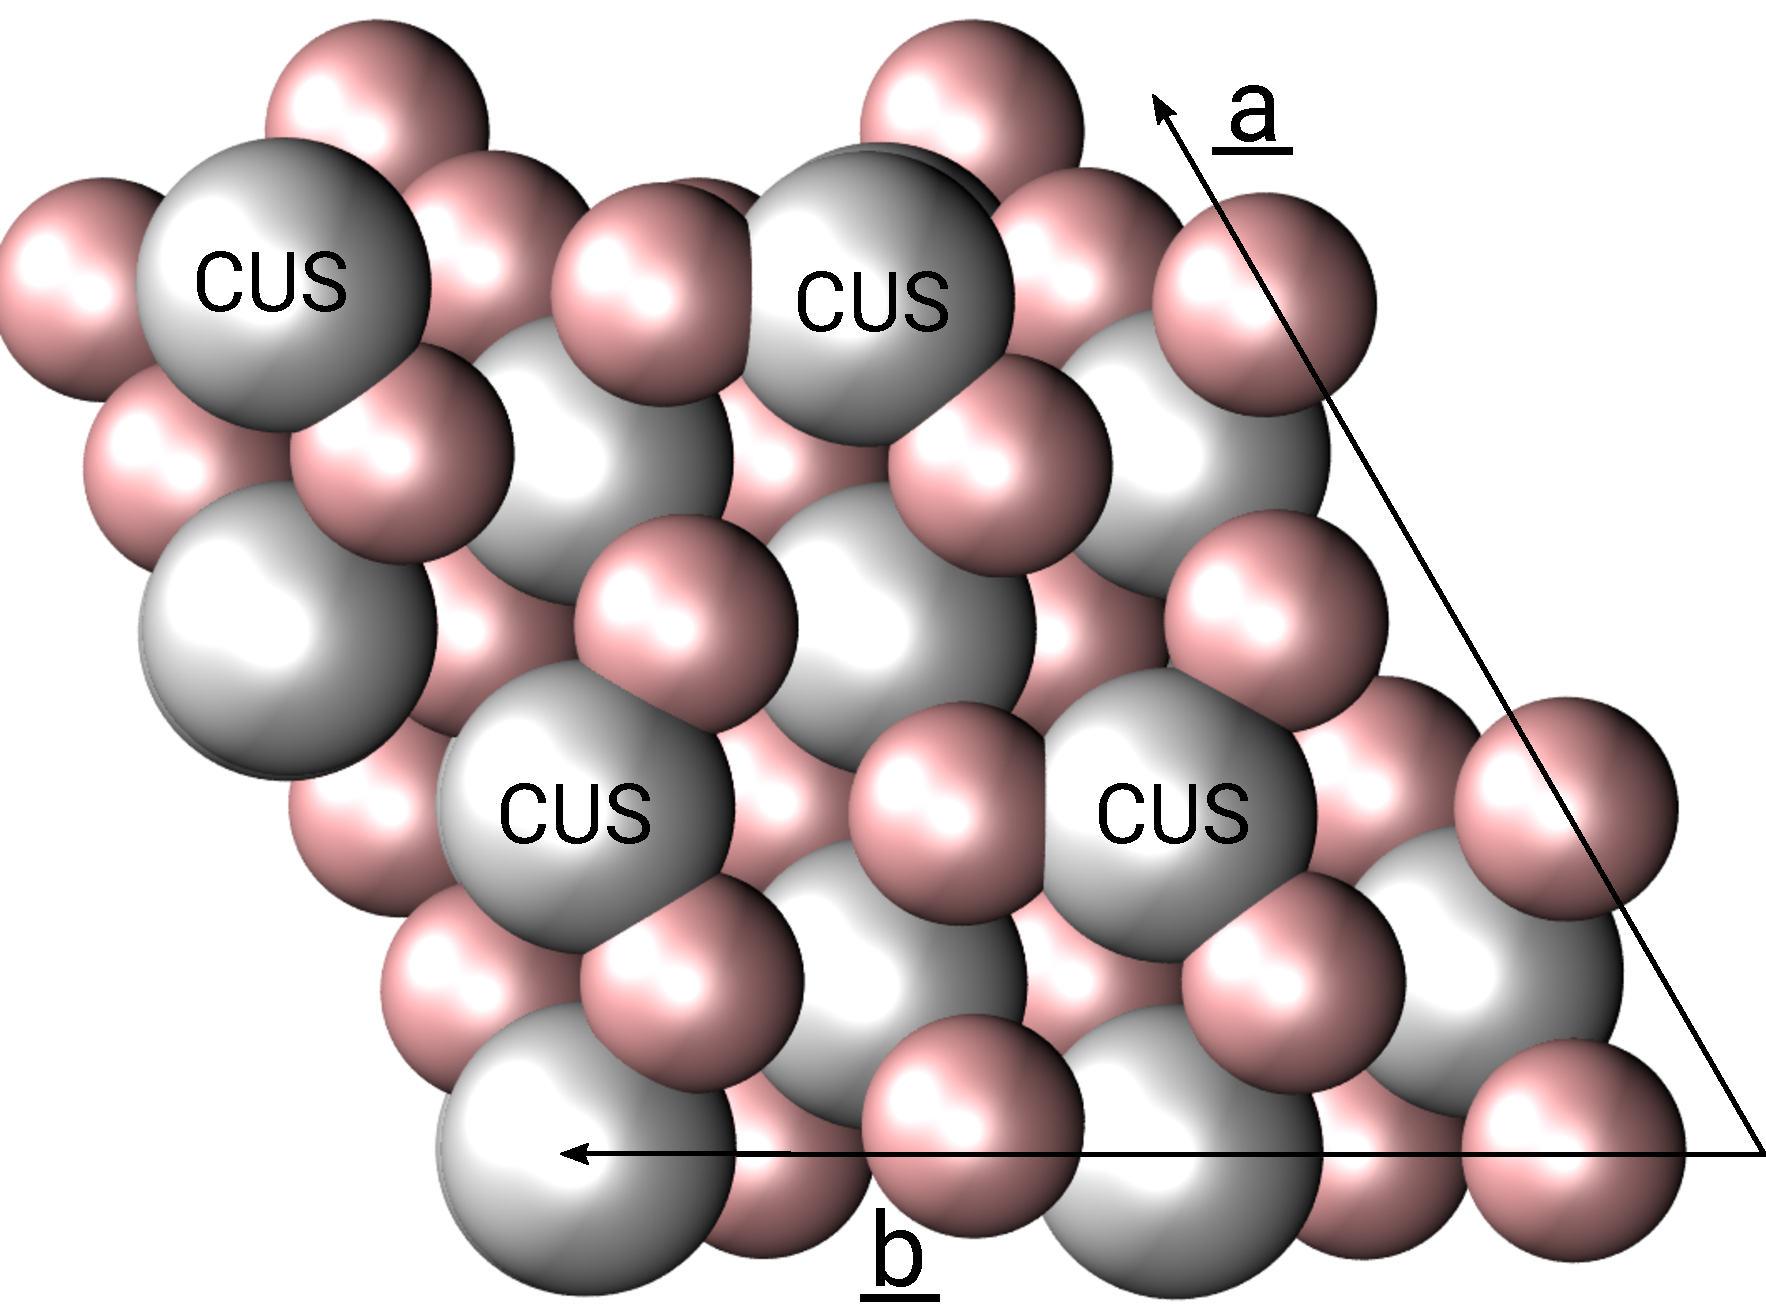
\includegraphics[width=0.45\textwidth]{figures/0001/surf_0K_axes.pdf}}
 \quad\quad
 \subfigure[(0001), side view]{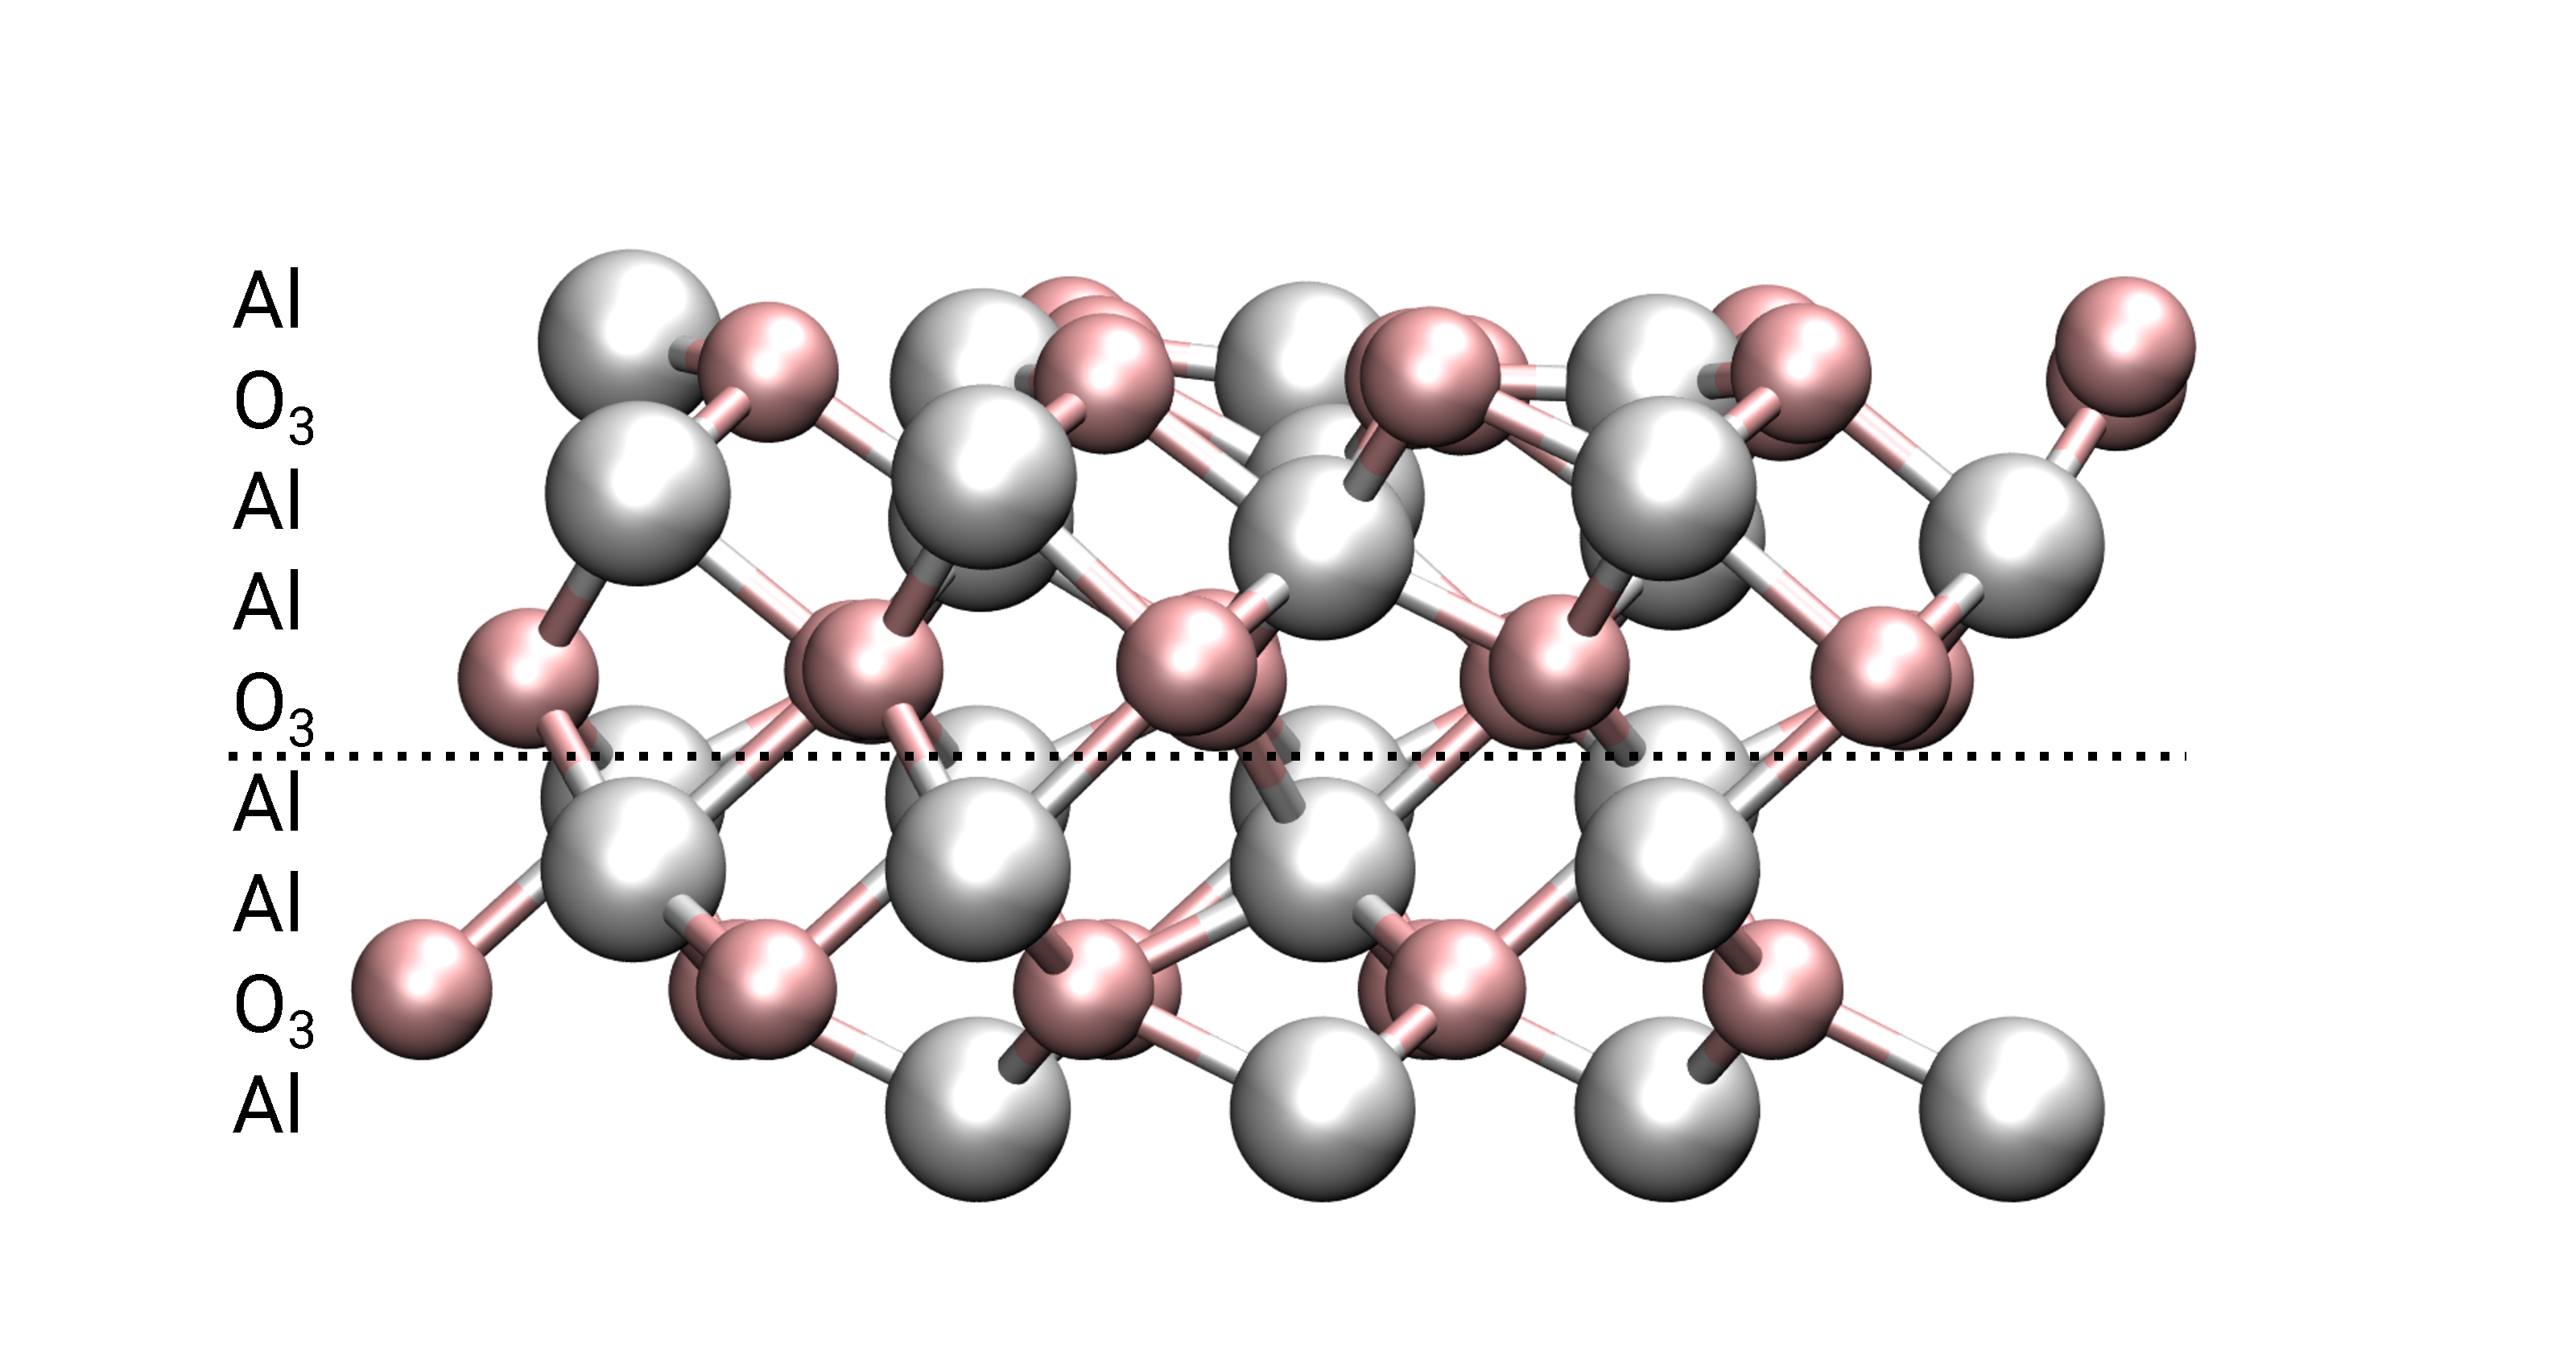
\includegraphics[width=0.45\textwidth]{figures/0001/surf_0K-side.pdf}}
 \caption{Surface model of the (0001), the most stable surface cur under UHV conditions. The top view (a) shows 4 Al CUS atoms, that are surrounded by three threefold coordianted surface oxygen atoms. (b) reveals the Al terminated surface cut in detail with the atomic layers.}
        \label{abb:surf_0001}
 \end{figure}

 \begin{figure*} [!ht]
\centering
\subfigure[mol]{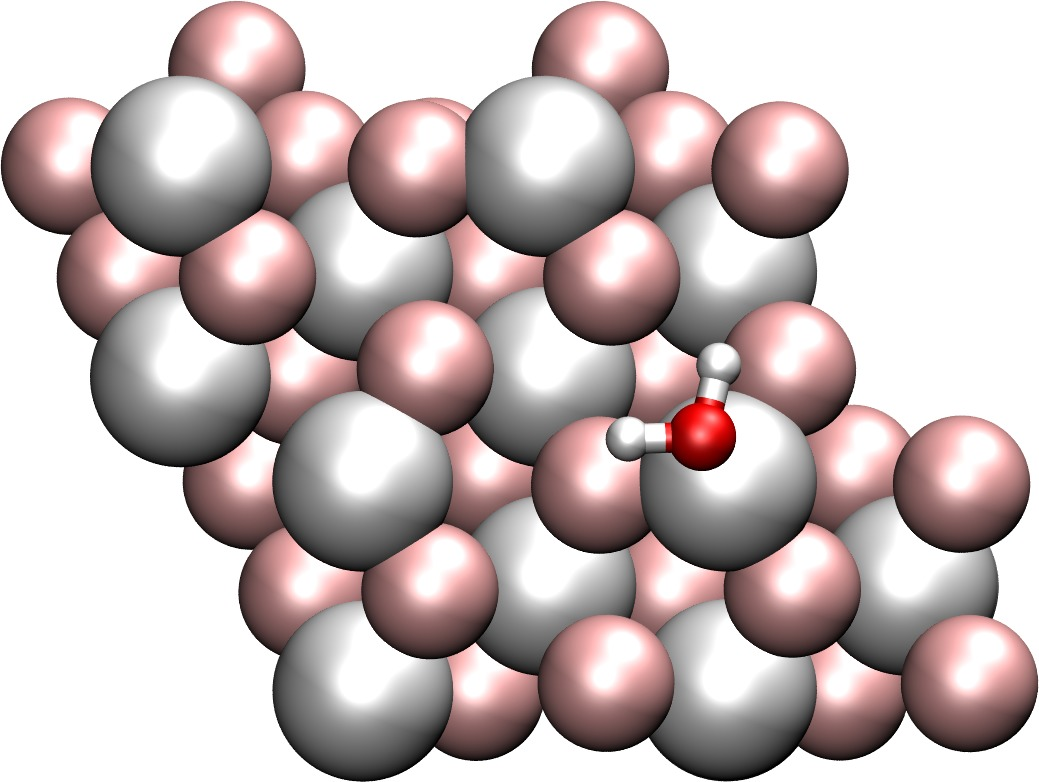
\includegraphics[width=0.4\textwidth]{figures/0001/0001_mol_top.jpg}}
         \quad
\subfigure[1-2]{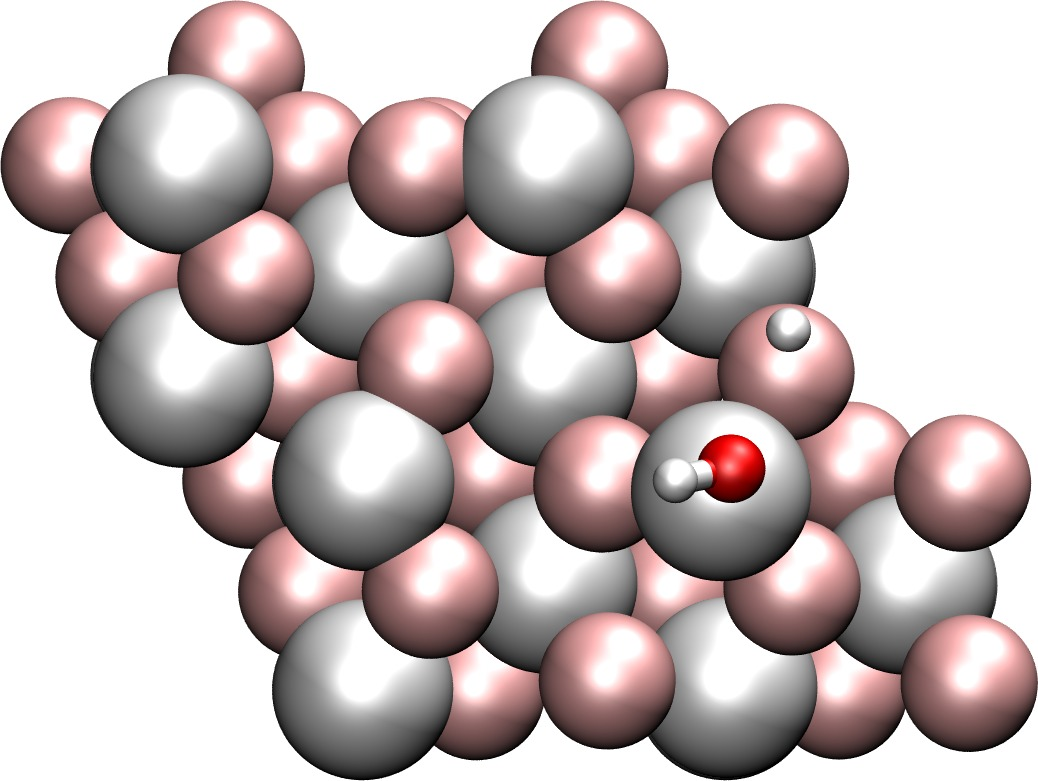
\includegraphics[width=.4\textwidth]{figures/0001/0001_1-2-diss_top.jpg}}
 \quad
\subfigure[1-4]{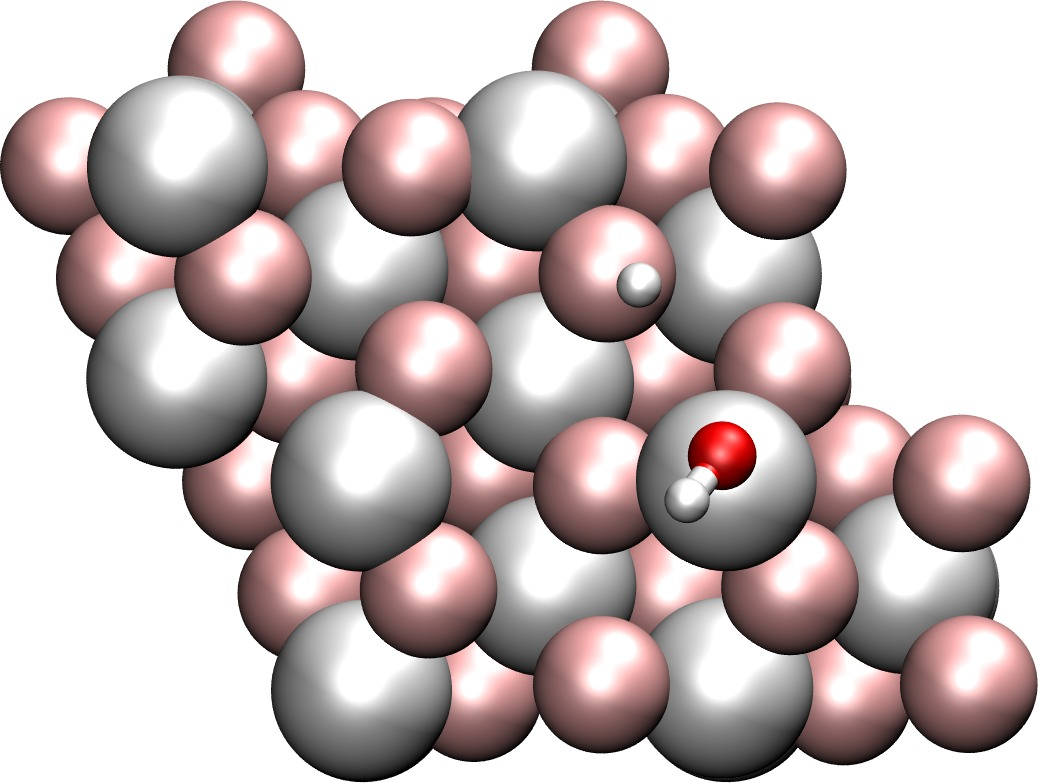
\includegraphics[width=.4\textwidth]{figures/0001/0001_1-4-diss_top.jpg}}
 \quad
\subfigure[1-4$^\prime$]{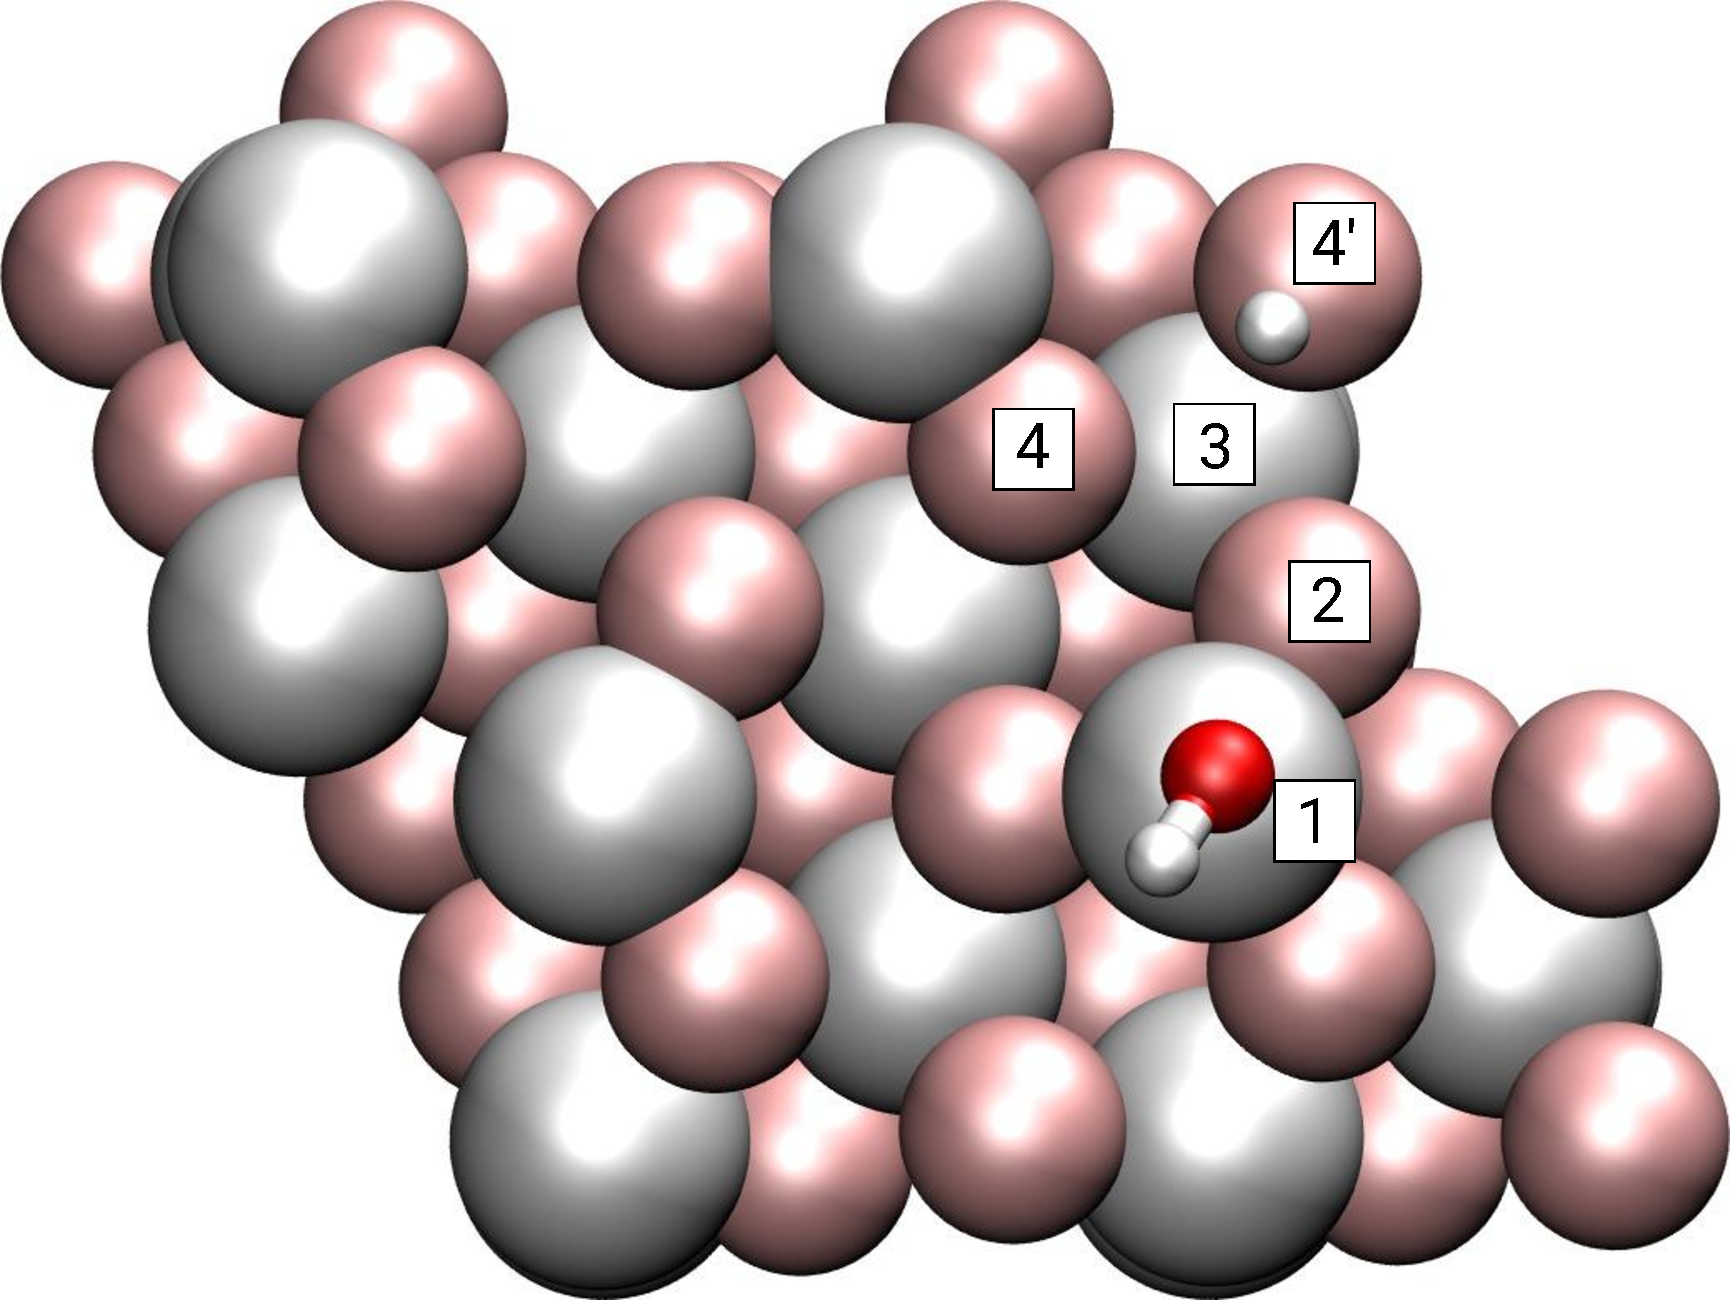
\includegraphics[width=.4\textwidth]{figures/0001/0001_1-4p-diss_top_label.pdf}}
\caption{Adsorption geometries of the molecular and the three dissociated species. Adsorption energies for these species can be found in Table \ref{tab:0001_eads+rates}.}
       \label{abb:0001_ads}
\end{figure*}
\section{AIMD for MBS Process}\label{sec_0001AIMD}
Intro, Hass, pinhole dosing vs. molecular beam source (= equilibrium situation vs non-equilibrium) higher dissociation probability, understanding these differences via AIMD. heavy water (D$_2$O) was used instead of H$_2$O to better compare with existing MBS experiments by R. K. Campen.
\\
{\color{red} Should I put the data in the appendix?}
%%%%%%%%%%OLD VERSION%%%%%%%%%%%%%%%%%
% Hass et. al. discussed the idea whether water will adsorb molecularly first and then dissociate or if direct dissociation upon adsorption is possible. To tackle this question for the experimental technique of the molecular beam source, we apply both microcanonical and canonical \textit{ab-initio} MD to simulate water in the beam approaching the surface. Interestingly, these experiments also show a higher disociation probability compared to pinhole dosing, that leads to an ensemble in thermal equilibrium, whereas MBS leads to a non-equilibrium situation. We start in the low coverage limit by letting one single, rigid molecule approach the $2\times 2$ supercell with only a linear momentum towards the surface. We later on continue with different approaches to more realistic beams and to more realistic surface situations. In the beam regime we probe water clusters, namely pre-optimized %(H$_2$O)$_2$ and
% (H$_2$O)$_4$ cluster, which is shot onto the surface. Another improvement to the beam lies in exciting the molecule either vibrationally and/or rotationally. These excitations were chosen from a normal mode analysis and the resulting stretch and bending modes.
% \\
% For improving the surface we first use a preequilibrated surface at $300\,$K, but also go to a surface situation in which already one water molecule is adsorbed. To pay attention to the equilibrium situation we considered a molecular preadsorbed water molecule,  the most stable 1-2 dissociated state as well as the 1-4 dissociated structure.
% \\
% We could show that water can both dissociate upon direct contact with the surface and also dissocioate after being adsorbed molecularly first and then after a time have enough energy to dissociate. This is mostly to the 1-2 dissociated state but also 1-4 and more surprisingly 1-4$^\prime$. It seems that the rotation of the water molecule before hitting the surface is crucial for direct dissociation. This energy can also be delivered by the heated surface, it has more energy in form of vibration, in this case prolongation of the respective OH bond and can therefore lead to dissociation. On the other hand hitting the surface directly on top of a CUS atoms was shown to lead mainly to reflection of the molecule, because the energy of the incoming molecule could not be absorbed by the surface.
% \\
% Trajectories with the vibrationally excited modes led to statistically higher levels of dissociation. Also temperature effects of the thermalized trajectories (canonical MD) seem to have a positive influence on the dissociation.
\subsection{Beam Model}
For the understanding of a Molecular Beam source experiment, the introduction of a beam is an essential part of the model. However, it was not possible to compute a fully realistic beam that was statistically converged, which would require wide knowledge about energy and velocity distributions and a systematic high dimensional sampling, that is not feasible with the computational power available at the moment. Instead as a first approach, a single, rigid water (D$_2$O) molecule (initial parameters are $d_{OD}=0.97$\AA~ and bond angle of $104.5$\textdegree) was sent perpendicularly from a center of mass position from a distance of $4\,$\AA~ onto the surface, in agreement with the experiment. Having these degrees of freedom excluded, from the 9 degrees of freedom, six are still left (see Figures \ref{abb:initial_parameters}, \ref{abb:impact_points} and Table \ref{tab:orientations}): two for the impact site [$a_0$,$b_0$] as it is given relative to the super cell vectors $\uline{a}$ and $\uline{b}$, three Euler angles $\alpha$, $\beta$ and $\gamma$ for the rotational orientation of the molecule with respect to the surface and the kinetic energy E$_\textrm{kin}$ that gives the molecule a momentum towards the surface, solely as translational motion, no vibration or rotation included. These parameters are varied systematically to gain insight into the process.
\\
As was mentioned before, the barriers can be high (and corresponding rates low), especially for the H-diffusion reactions, but the adsorption process itself is barrierless, and additionally the incoming water molecule has kinetic energy so that processes, that are slow at room temperature otherwise, can be speeded up.
\\
Further improvements of this simplest model are made in subsections \ref{clusters} and \ref{preex}, that address clustering and rotational and vibrational excited water, respectively. Further details are given there.

\begin{figure}[!ht]
 \centering
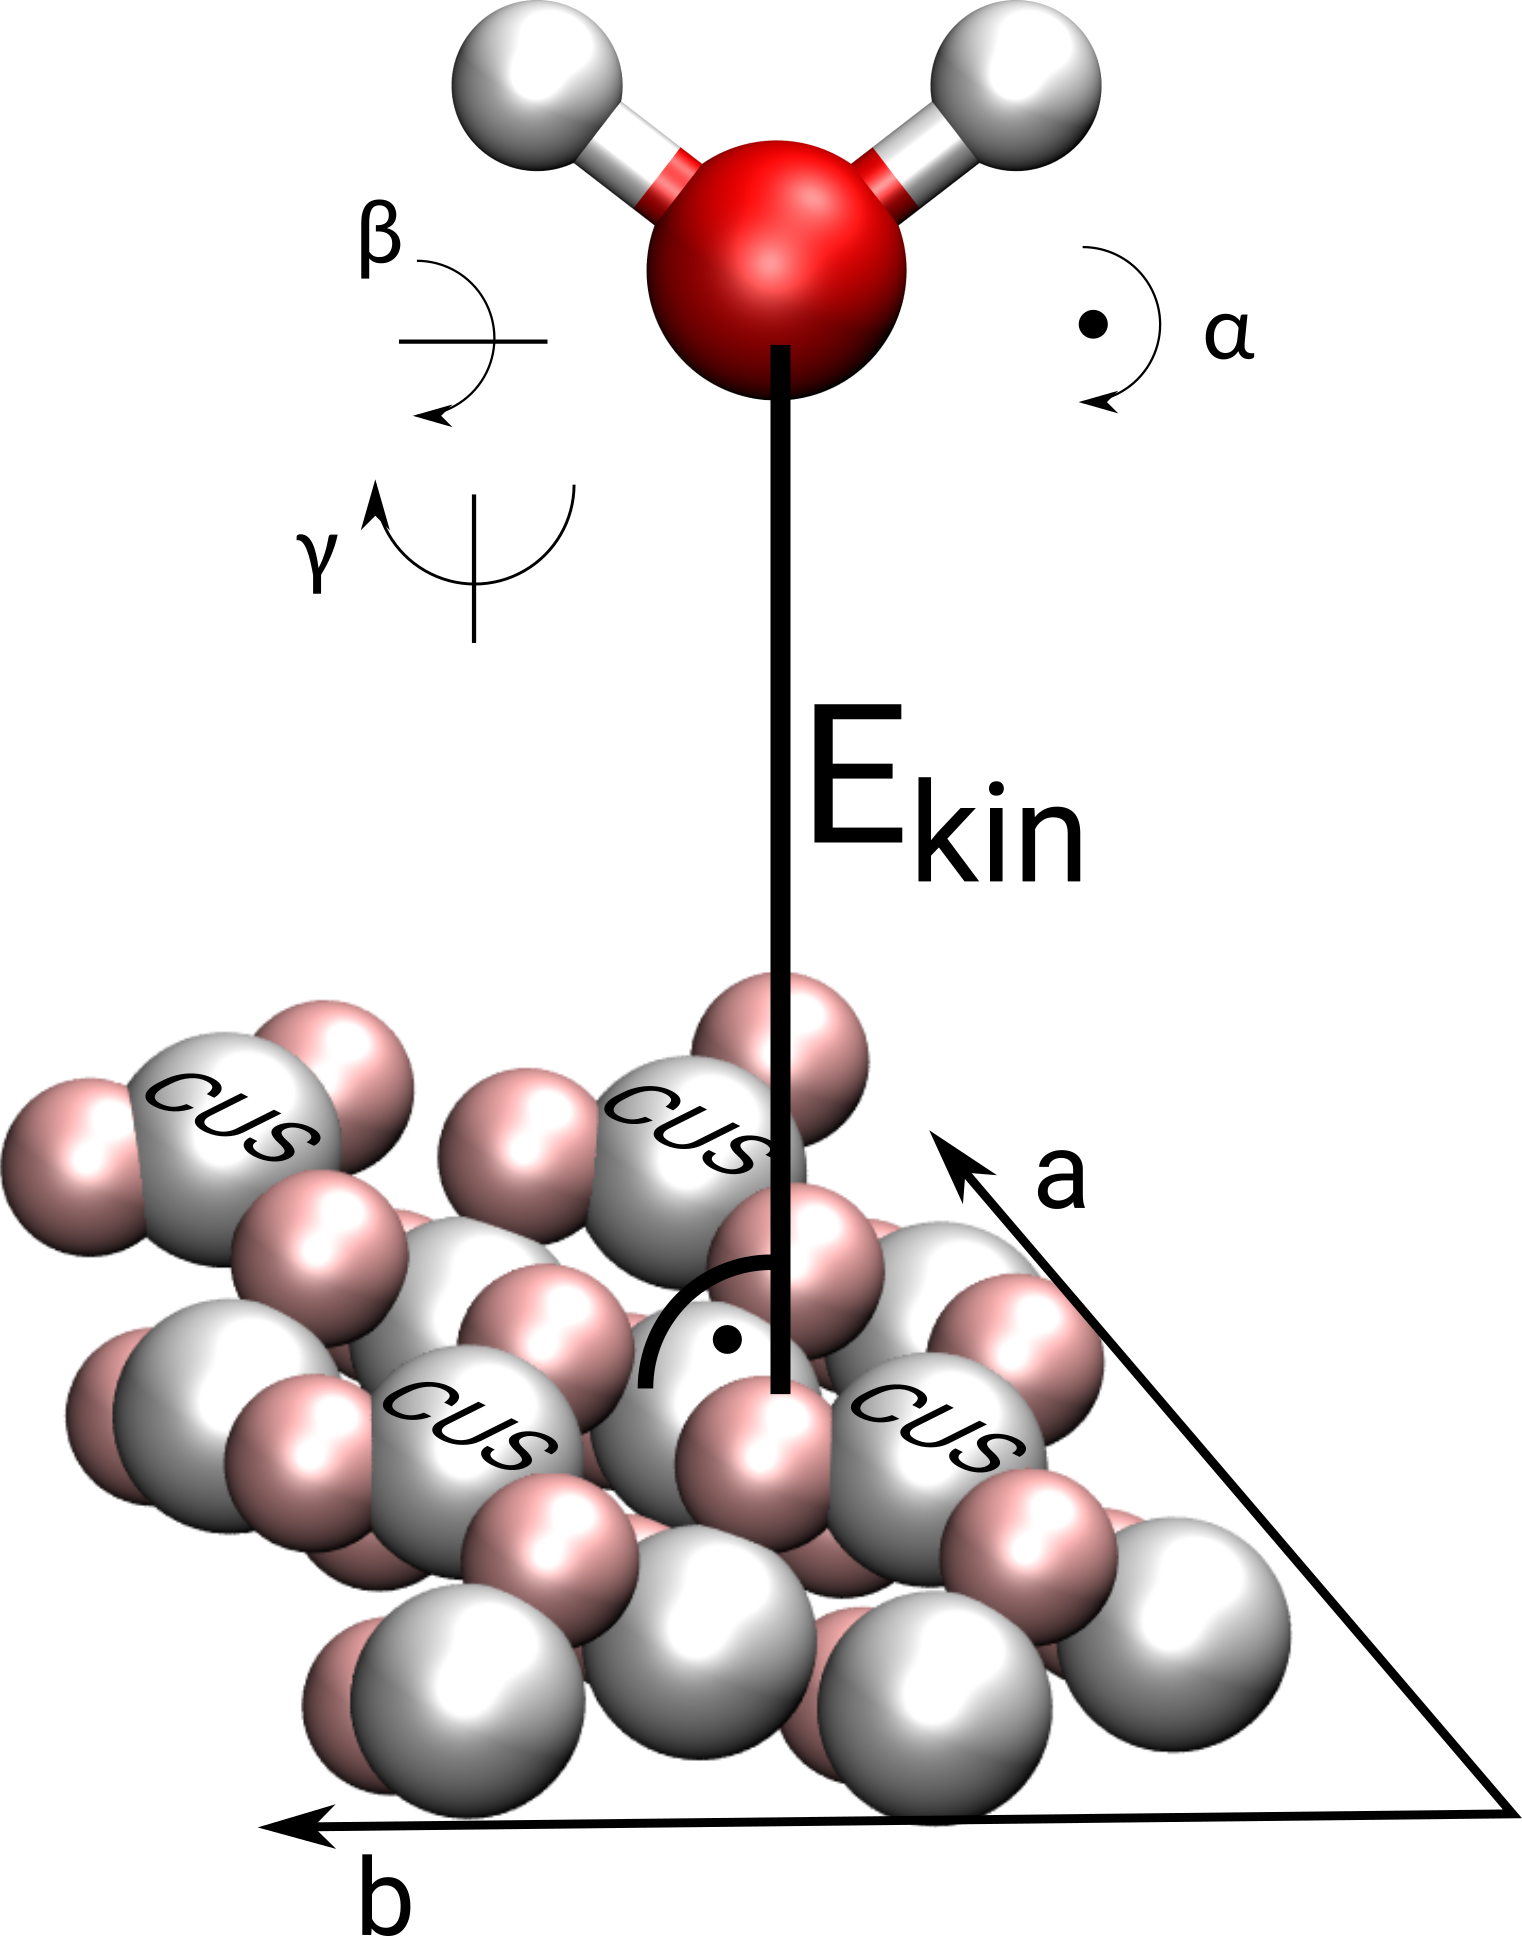
\includegraphics[width=0.3\textwidth]{figures/0001/perspective+h2o_new.png}
 \caption{Sketch for inital parameters of the trajectories. The water molecule is situated $4\,$\AA{} above the surface and is arranged within the shown coordinate system, before being shot onto the surface with a defined kinetic energy E$_\textrm{kin}$.}
        \label{abb:initial_parameters}
 \end{figure}
 
 \begin{figure}[h!]
 \centering
 \subfigure[{[0.33,0.33]}]{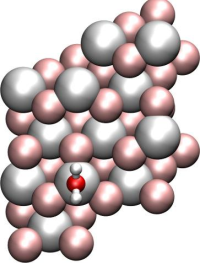
\includegraphics[angle=90, scale=0.45]{figures/0001/0_33-0_33test.png}}
          \quad
 \subfigure[{[0.5,0.5]}]{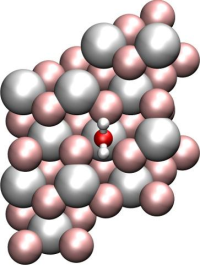
\includegraphics[angle=90,scale=0.45]{figures/0001/0_5-0_5test.png}}
         \quad
 \subfigure[{[0.35,0.5]}]{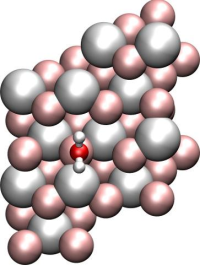
\includegraphics[angle=90,scale=0.45]{figures/0001/0_35-0_5test.png}}
        \\
 \subfigure[{[0.5,0.35]}]{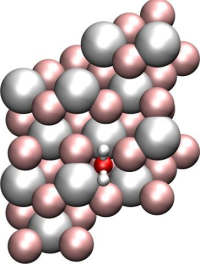
\includegraphics[angle=90,scale=0.45]{figures/0001/0_5-0_35test.png}}
        \quad
 \subfigure[{[0.35,0.45]}]{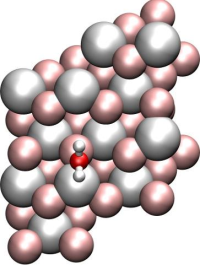
\includegraphics[angle=90,scale=0.45]{figures/0001/0_35-0_45test.png}}
        \quad
 \subfigure[{[0.4,0.5]}]{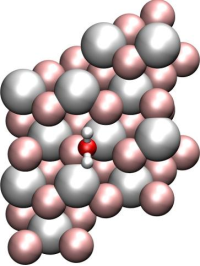
\includegraphics[angle=90,scale=0.45]{figures/0001/0_4-0_5test.png}}
 \caption{The six impact points $[a_0,b_0]$ that were used in the AIMD calculations (shown for the rotational orientation $[0,0,0]$, topview).The different points reflect the most important sites of the surface, [0.33,0.33] is on top of an Al CUS, [0.5,0.5] on top of an Al in a lower layer. [0.35,0.5] is on top of a surface oxygen atom, whereas [0.5,0.35] is on top of a subsurface oxygen atom. [0.35,0.45] is in a gap between an Al CUS and a surface oxygen and [0.4,0.5] is in the gap between a surface O and a subsurface Al atom.}
        \label{abb:impact_points}
 \end{figure}
 
 \begin{table}[!h]
 \centering
  \caption{Orientations of the water molecule. Shown are both top view and side view at impact point 0.5,0.5. (look from the right-hand side to the top view)}
 \begin{tabular}{cp{4cm}p{4cm}}
 orientation ($\alpha,~\beta,~\gamma$)& top view & side view \\\hline
 (0, 0, 0)  & 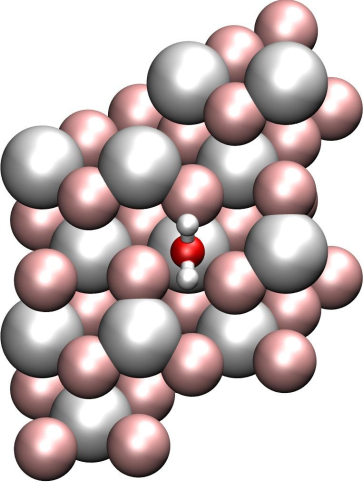
\includegraphics[width=2cm,angle=90]{figures/0001/Ausrichtungsbilder/0_0_0-toptest.png}
&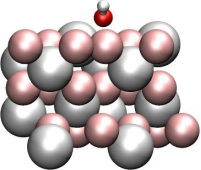
\includegraphics[width=2.5cm]{figures/0001/Ausrichtungsbilder/0_0_0-sidetest.png}\\
(0, 0, 90)   & 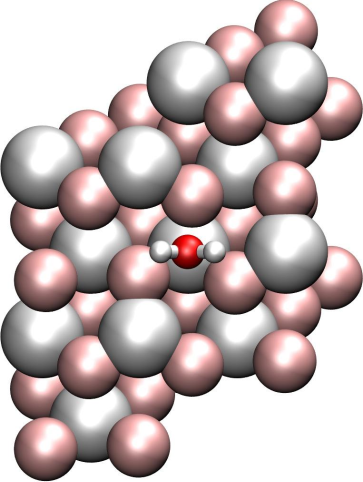
\includegraphics[width=2cm,angle=90]{figures/0001/Ausrichtungsbilder/0_0_90-toptest.png}
& 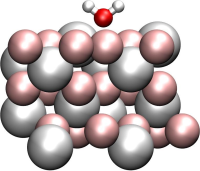
\includegraphics[width=2.5cm]{figures/0001/Ausrichtungsbilder/0_0_90-sidetest.png}\\
(0, 90, 0)   & 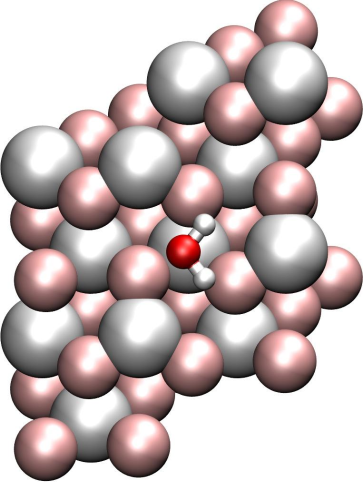
\includegraphics[width=2cm,angle=90]{figures/0001/Ausrichtungsbilder/0_90_0-toptest.png}
& 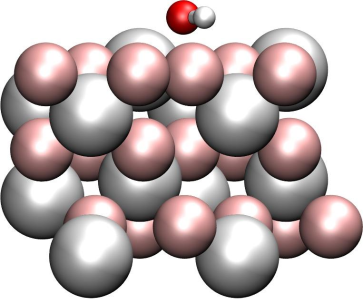
\includegraphics[width=2.5cm]{figures/0001/Ausrichtungsbilder/0_90_0-sidetest.png}\\
(0, 90, 90) & 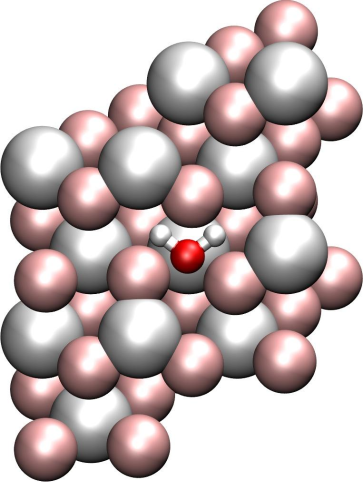
\includegraphics[width=2cm,angle=90]{figures/0001/Ausrichtungsbilder/0_90_90-toptest.png} 
& 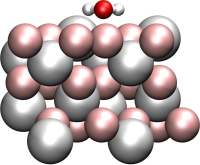
\includegraphics[width=2.5cm]{figures/0001/Ausrichtungsbilder/0_90_90-sidetest.png}\\
(90, 0, 0) &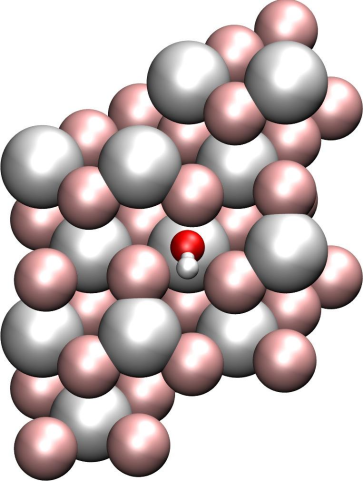
\includegraphics[width=2cm,angle=90]{figures/0001/Ausrichtungsbilder/90_0_0-toptest.png} 
& 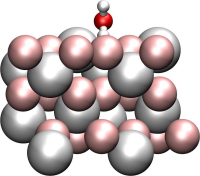
\includegraphics[width=2.5cm]{figures/0001/Ausrichtungsbilder/90_0_0-sidetest.png}\\
(90, 0, 90) & 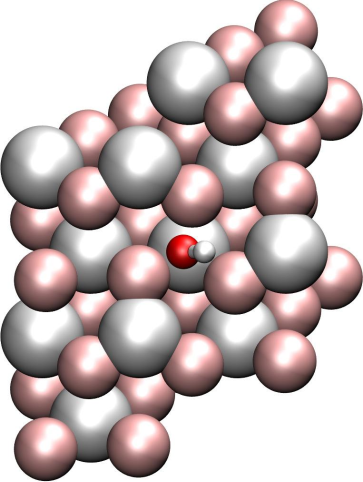
\includegraphics[width=2cm,angle=90]{figures/0001/Ausrichtungsbilder/90_0_90-toptest.png} 
& 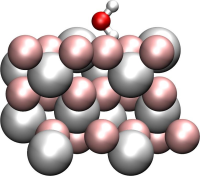
\includegraphics[width=2.5cm]{figures/0001/Ausrichtungsbilder/90_0_90-sidetest.png}\\
(90, 90, 0) &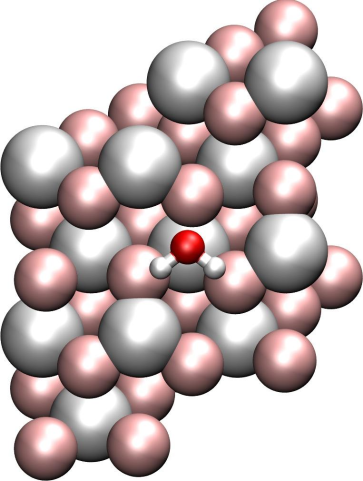
\includegraphics[width=2cm,angle=90]{figures/0001/Ausrichtungsbilder/90_90_0-toptest.png} 
& 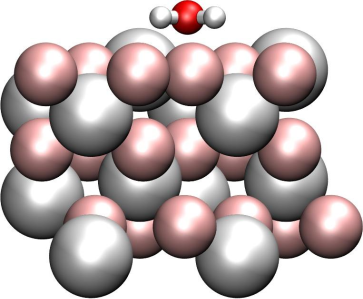
\includegraphics[width=2.5cm]{figures/0001/Ausrichtungsbilder/90_90_0-sidetest.png}\\
(90, 90, 90) & \includegraphics[width=2cm,angle=90]{figures/0001/Ausrichtungsbilder/90_90_90-toptest.png} 
& \includegraphics[width=2.5cm]{figures/0001/Ausrichtungsbilder/90_90_90-sidetest.png}\\
\end{tabular}
 \label{tab:orientations}
\end{table}
 
\subsection{Example Trajectories}
Before going to the details, example trajectories for each process leading to one of the four most stable adsorbed species, molecular adsorption, 1-2 dissociation, 1-4 dissociation and 1-4$^\prime$ dissociation are shown in Figure \ref{abb:ex_traj}, the applied parameters are reported in the respective caption. These figures were all obtained from canonical calculations (NVT) at $300\,$K (see Figure \ref{abb:ex_traj}, the trajectory shown in (d) was additionally preexcited in the asymmetric stretch mode leading to 1-4$^\prime$ dissociation). As one can see, molecular, 1-2 and 1-4 dissociated species can occur directly at the impact time of the water molecule at the surface and is henceforth called direct dissociation from the gas phase. For the 1-4$^\prime$ dissociation shown in Fig.~\ref{abb:ex_traj}(d), this process does not happen directly at the impact but (in this case) ca. $40\,$fs later, so this is referred to as indirect dissociation with a molecular intermediate. This indirect process is not unique for the 1-4$^\prime$ dissociated species, all the other species including the molecular can be observed to happen indirectly by either being reflected first from the surface before adsorbing/dissociating or by adsorbing molecularly before dissociating. However, the 1-4$^\prime$ species was the only one that could not be observed after direct dissociation.

  \begin{figure}[h!]
\begin{center}
\hspace*{-1cm}
\begin{tabular}{cc}
\hspace*{-1cm}
(a) molecular adsorption & (b) 1-2 dissociation \\
{\includegraphics[width=0.4\textwidth]{figures/0001/graphs/mol.eps}}
         &
{\includegraphics[width=0.4\textwidth]{figures/0001/graphs/1-2.eps}} \\
 (c) 1-4 dissociation & (d) 1-4' dissociation \\
{\includegraphics[width=0.4\textwidth]{figures/0001/graphs/1-4.eps}} &
{\includegraphics[width=0.4\textwidth]{figures/0001/graphs/1-4d.eps}}
\end{tabular}
\end{center}
\caption{{\color{blue} Examplary trajectories for trajectories of different initial parameters, leading to the four adsorption states of water at the $\upalpha$-Al$_2$O$_3$(0001) surface as indicated in Figs.\ref{abb:0001_ads}(a)-(d). For all cases these are canonical (NVT) trajectories at  $T=300$ K. The initial parameters: (a) $E_\textrm{kin}=0.7$ eV, $[a_0,b_0]=[0.33,0.33]$, $[\alpha,\beta,\gamma]=[0,0,90]$ (in \textdegree);
 (b) $E_\textrm{kin}=0.7$ eV, $[a_0,b_0]=[0.35,0.45]$, $[\alpha,\beta,\gamma]=[0,0,0]$;
 (c) $E_\textrm{kin}=0.7$ eV, $[a_0,b_0]=[0.33,0.33]$, $[\alpha,\beta,\gamma]=[0,90,0]$;
 (d) $E_\textrm{kin}=0.7$ eV, $[a_0,b_0]=[0.35,0.5]$, $[\alpha,\beta,\gamma]=[0,0,0]$, and the water molecule 
 was vibrationally preexcited along the asymmetric stretch normal coordinate as specified in Subsec. \ref{preex}. The $r$ values indicate bond lengths between water-O and the CUS Al atom on which either D$_2$O or the water hydroxyl unit OD adsorb (O-Al), the distance between water-O and D in non-dissociated (fragments of) D$_2$O (O-D or O-D$_\textrm{ads}$), and the  distance between water-O and D in dissociated (fragments) of D$_2$O (O-D$_\textrm{diss}$), respectively. The corresponding interatomic distances of the adsorbed species from the static DFT calculations reported in Figs.\ref{abb:0001_ads}(a)-(d) are shown as horizontal, dashed lines. In (d), the 1-4$^\prime$ state is reached \textit{via} a 1-2 dissociation intermediate, which is very short-lived around $0.1\,$ps.}}
\label{abb:ex_traj}
\end{figure}

\subsection{Microcanonical AIMD at clean surface}\label{sec:mic_clean}
{\color{red} All those tables in the appendix?}\\
The effects of a single D$_2$O shot to the cool surface with a NVT ensemble (microcanonical AIMD) were studied systematically by probing over 5 different kinetic energies (from $0.5$ to $0.9\,$eV in $0.1\,$eV steps), six lateral impact points at the surface ([0.33,0.33], [0.5,0.5], [0.35,0.5], [0.5,0.35], [0.35,0.45], [0.4,0.5], see also Figure \ref{abb:impact_points}) and eight different orientations of the water with respect to the surface ([0,0,0], [0,0,90], [0,90,0], [0,90,90], [90,0,0], [90,0,90], [90,90,0], [90,90,90], see also Tab.\ref{tab:orientations}). These $5\times 6\times 8=240$ AIMD trajectories for the clean surface at $T=0\,$K were carried out for ca $1.2\,$ps each.
\\
In the trajectories  either molecular adsorption, 1-2 dissociation or reflection could be observed. Dissociation was assumed, if the OD distance was greater than $1.3\,$\AA{}, but it was made sure that the results did not differ for a greater cutoff distance. Interestingly, only 1-2 dissociation and no 1-4 dissociation could be observed for the conditions (NVT, clean surface), although the molecular and the 1-4 dissociated species are almost equal in energy, and also the barrier heigths for the dissociation to 1-2 ($0.13\,$eV) and 1-4 ($0.19\,$eV) do not differ largely. As it is shown later, other conditions are necessary for reaching 1-4 dissociation.
\\
  \begin{figure}[h!]
\centering
 \subfigure[Energy]{\includegraphics[width=0.3\textwidth]{figures/0001/graphs/E.png}} 
 \quad
 \subfigure[Impact Point]{\includegraphics[width=0.3\textwidth]{figures/0001/graphs/impactpoint.png}} 
 \quad
 \subfigure[Orientation]{\includegraphics[width=0.3\textwidth]{figures/0001/graphs/orientation.png}}
\caption{{\color{blue} Statistics of AIMD trajectories at $T=0$ (NVE), for single D$_2$O approaching a clean alumina(0001) surface. In (a), for each of the five different initial kinetic energies $E_\textrm{kin}$, results are averaged over the $6 \times 8=48$ combinations of impact sites and rotational orientations. In (b), for each of six different initial impact points $[a_0,b_0]$, results are averaged over $5 \times 8=40$ combinations of kinetic energies and rotational orientations. In (c), each of the eight different initial rotational orientations $[\alpha,\beta,\gamma]$, results are averaged over $5 \times 6=30$ combinations of kinetic energies and impact points. Columns show percentages of trajectories leading to  reflection (``refl''), molecular adsorption (``mol''), and  direct and total 1-2 dissociation (``1-2 diss direct'' and  ``1-2 diss total''). (No columns if no trajectories of the  type were found.)}}
\label{abb:barchart_mic}
\end{figure}
For a statistical analysis of the data see Figure \ref{abb:barchart_mic}, where the probabilities for reflection, molecular adsorption and 1-2 dissociation are shown as a function of the kinetic energy (a), impact point (b) and the orientation (c). There also between direct and indirect dissociation is distinguished. Admittedly, this analysis is restricted by the number of trajectories (240). From these figures and the data one can derive the following conclusions:
\\
As anticipated, all three processes could be observed, reflection ($20.4\%$, 49 of the 240 trajectories), molecular adsorption ($55.4\%$, 133 trajectories) and 1-2 dissociation ($24.2\%$, 58 trajectories).
\\
Looking at the impact of the energy in Fig.~\ref{abb:barchart_mic}(a), the result do not depend largely on the initial kinetic energy of the molecule, at least for the probed energy range. In all cases molecular adsorption dominates, followed by 1-2 dissociation and reflection, that are in the same range around $20$-$25\%$. This reflecion probability P$_\textrm{diss}$ is only increased for $0.9\,$eV, at the expense of the molecular species. To tackle the low energy regime, one additional trajectory of $0.1\,$eV was done ([$a_0,b_0]=[0.35,0.45]$; $[\alpha,\beta,\gamma]=[0,0,0]$), for which $P_\textrm{diss}=1$ for all energies $\geq 0.5\,$eV. In the case of E$_\textrm{kin}=0.1\,$eV, the trajectory only shows molecular adsorption. This result was rather surprising, since the kinetic energy plus the adsorption energy minus the barrier height is with ($0.1+1.31-0.13$)eV=$.28\,$eV larger than the reaction barrier. It seems that the excess energy is not available for the OD-bond breaking and instead relaxes in other degrees of freedom of the system. That allows to draw the conclusion, that a minimum kinetic energy is necessary for the dissociation process. In the experiments of R. K. Campen, a kinetic energy of the beam between $0.6$ and $0.75\,$eV is used. This minimum energy constraint can be one possible explanation of the difference between MBS and pinhole dosing. In the latter case, the only energy of a water molecule comes from the thermal energy that is for a D$_2$O molecule in the gas phase at $300\,$K around $\frac{3}{2}k_BT\approx40\,$meV.
\\
In contrast to the kinetic energy, the lateral impact point at the surface has a great influence on adsorption and dissociation probabilities (see Fig.~\ref{abb:barchart_mic}). For the impact point [0.5,0.5], that is at a  non-surface Al position, $88\%$ of the trajectories get reflected and molecular adsorption and 1-2 dissociation are oppressed, whereas for [$0.33,0.33$], directly on top of an Al CUS position, $83\%$ adsorb molecularly which dominates clearly over 1-2 dissociation. In contrast to both sites, [$0.35,0.45$] which is a gap between a CUS position and a neighboring oxygen atom leads to a high dissociation probability of P$_\textrm{diss}\approx 68\%$ with a minor percentage of indirect dissociation. This high dissociation probability can be explained by the fact, that the molecule hits the surface already in a ``product-like'' geometry, so that the OD bond breakage is facilitated.
\\
The initial rotational orientation has also an effect, although not so clearly as for the impact point. This might be explained when looking at the trajectories in detail, so one can see, that the water molecule rotates due to the attractive and repulsive interaction with the surface atoms, that lead to a reorientation of the water molecule right before adsorbing, so that the initial orientation is not remembered by the system. The orientation that the molecule is in shortly before reaching the surface is more important, also here, if the molecule's orientation is already in a product-like state, the dissociation probability is elevated.
\\
As can be seen from the data, direct dissociation dominates mostly over indirect dissociation, although it is dependend from the initial conditions, e.g. for the initial orientation [0,90,90] only indirect dissociation is observed (cf. Fig.~\ref{abb:barchart_mic}(c)).

 
\subsection{Thermalized Surface}\label{therm_surf}
After getting an impression about the system with the microcanonical MD with the clean surface, as a next step the thermalized surface at $300\,$K is studied. For this the naked surface was preequilibrated at $300\,$K for $1\,$ps and the obtained geometry with the included velocities was used as an input to the following calculations. Here, only a kinetic energy of $0.7\,$eV was considered, since this energy is the closest to previous experiments by Kramer and also the energy dependence was shown to be very low. The water molecule was then shot onto the equilibrated surface and the heat bath acted from the start on the water molecule. This is not a problem, since the molecule hits the surface quickly and thus hardly affects the dynamics.
\\
First, for a selection of 5 parameter sets 100  NVT trajectories were calculated each at a temperature of $300\,$K. These parameter sets are $[a_0,b_0][\alpha,\beta,\gamma]$= $[0.35,0.45]$,$[0,0,0]$; $[0.35,0.45]$,$[0,90,90]$; $[0.35,0,45]$,$[90,90,90]$; $[0.4,0.5]$,$[0,0,0]$;  $[0.5,0.35]$,$[90,0,90]$. These parameters led in the previous microcanonical ensemble to 1-2 dissociation and were chosen because the idea was that the thermal effects might trigger them to dissociate or diffuse to the 1-4 species. The duration of the trajectories was $1\,$ps and were done analogously to \ref{sec:mic_clean} except for now the thermalized surface. All of these 500 trajectories dissociated 1-2, no reflection, molecular adsorption or further dissociation could be observed. As it seems, the thermal contribution is low, which was unexpected. The energy of the thermalized surface can be estimated by $N_s\times 3k_BT=2.8\,$eV (with $N_s=36$ being the number of atoms in the surface slab that were allowed to relax/move). This energy is in the same range as the kinetic energy of the incoming water molecule ($\approx2\,$eV). Indeed, this surface energy is not valid for the small surface range where the impact takes place, so that the thermal energy of the atom(s) of the impingement is considerably smaller.
\\
As a next step, for all $6\times 8=48$ combinations of parameters, but with the thermalized surface, were done for all 6 impact points and 8 orientations presented in Section \ref{sec:mic_clean}, but only for a kinetic energy of $0.7\,$eV. For each of the sets, two trajectories of $4\,$ps duration were calculated. This restriction is due to high computational costs and  gives rise to only a limited statistical significance. The long duration accounts for processes that occur later after the impact, that could have been missed by shorter trajectories. In Table \ref{tab:nvt-nve_comp}, the probabilities for each process is shown, in comparison with the previous microcanonical AIMD trajectories. Because 6 of the trajectories aborted due to numerical reasons, here only 42 trajectories can be evaluated and the comparison is, of course, done only with the corresponding microcanonical trajectories.
\begin{table}[!h]
 \centering
 \caption{{\color{blue} Statistics for NVE (upper two lines) and NVT ($T=$ 300 K, lowest line) AIMD trajectories. The initial impact parameters $[a_0,b_0]$ and $[\alpha,\beta,\gamma]$ were (selected from) the 48 impact parameters used in Sec. \ref{sec:mic_clean} as desribed in the text. In all cases, a single water molecule with initial $E_\textrm{kin}=0.7$ eV was fired on a clean surface.}}
\vspace*{.2cm}
  \begin{tabular}{lc|cccc}
 \hline
  ensemble & no. of trajectories & $P_\textrm{refl}$ & $P_\textrm{mol}$ & $P_\textrm{diss}$ (1-2) & $P_\textrm{diss}$(1-4) 
 \\\hline
 NVE$^1$         & 48 & 0.19 & 0.58 & 0.23 & 0.00 \\
 NVE$^{1,3}$     & 42 & 0.19 & 0.55 & 0.26 & 0.00 \\
 NVT$^2$ &$42\times 2$& 0.12 & 0.54 & 0.24 & 0.11 \\\hline
  \end{tabular}
\begin{tablenotes}
 \footnotesize
\item[] $^1$ Propagation time $1.22$ ps. $^2$ Propagation time 4 ps. $^3$ A subset of the NVE/48 data set,  corresponding to the same initial impact parameters as used for the NVT ensembles.
\end{tablenotes}
\label{tab:nvt-nve_comp}
\end{table}
In the first line of the table, the results for the complete probed space for the NVE (T=0) is shown, the second line gives the results for the corresponding 42 microcanonical trajectories and in the third line, the canonical results for 42 NVT trajectories ($T=300\,$K) are given. For all, the kinetic energy is $E_\textrm{kin}=0.7\,$eV. In contrast to the microcanonical MD, the canonical show 1-4 dissociation at a percentage of around $11\%$ and slight decreases in the reflection, whereas molecular adsorption and 1-2 dissociation almost are equal. From the 1-4 dissociated trajectories, $44\%$ dissociated directly and $56\%$ indirectly after initial molecular adsorption. Interestingly, all inital conditions in the trajectories that show 1-4 dissociation in the NVT led only to molecular adsorption in the NVE AIMD.
\\
Note, that the surface temperature indeed has an effect on the probabilities for the different processes and also 1-4 dissociation could be observed.
As before, the first impact can lead to reflection and in a ``bouncing'' process, the molecule can also adsorb after another impact, in some cases also on another CUS atom as the initial impact was on.
 
\subsection{Refined Surface Model}
In the experiment, after a certain time, the coverage will be higher, which will have an impact on the incoming molecule. To account for this a preadsorbed surface model was applied, where the minimum structure of the surface with a single adsorbed water molecule was used and a second D$_2$O was sent onto this surface. For the preadsorbed water, the three minima were assumed: (a) the molecular minimum, (b) the 1-2 dissociated species and (c) the less stable 1-4 dissociated water. The preadsorbed OD/D$_2$O was adsorbed at the position [0.33,0.33], in the lower right $1\times 1$ sub cell of the super cell in Figure \ref{abb:0001_ads}, that is located around the CUS atom at this lateral impact point.
\\
For the incoming second water molecule with an initial kinetic energy of $0.7\,$eV, one has to distinguish two cases: The impact points [$a_0,b_0$] were chosen such that (i) the second water molecule is shot in the same $1\times 1$ sub cell where the preadsorbed water is adsorbed (the lower right part of the super cell) and (ii) in another sub cell, here, the lower left part. Once again, various initial orientations and impact points were probed for a propagation time of $1\,$ps.
\\
First, NVE (microcanonical, $T=0\,$K of the initial surface) were done. (i) In the first case, the incoming water is shot to the vecinity (same sub cell) of the preadsorbed molecular water, the second \textit{incoming} D$_2$O is observed to be either reflected or adsorb molecularly at another CUS atom after initial reflection from the preadsorbed water molecule. In the case of molecular preadsorbed water, the impact of the second molecule can make the molecular \textit{preadsorbed} water dissociate to 1-2, 1-4 and even 1-4$^\prime$. Assumingly, part of the energy is not used to overcome the barrier to diffusion/dissociation but to interaction with the preadsorbed molecular species. The same does not happen for the 1-2 and the 1-4 preadsorbed species only in one case reacts to the molecular adsorbed species. As can be seen in Table \ref{tab:preads_mic}, there is a difference between impact points direct on the CUS atom ($[0.33,0.33]$) and the impact position next to the CUS position $[0.35,0.45]$. Additional data is shown in the Appendix.
\begin{table}[!h]
  \centering
  \caption{{\color{blue} Outcome of selected microcanonical (NVE, $T=0$) trajectories with $E_{\textrm{kin}}=0.7\,$eV, after the end of propagation, for three cases of a single water molecule being molecularly or dissociatively preadsorbed on the surface. R=reflection, M= molecular adsorption (chemisorption), P=molecular physisorption, D(1-2)=1-2 dissociation, D(1-4)=1-4 dissociation. In each entry, the first letter gives the outcome for the \textit{incoming} molecule, the second one the fate of the preadsorbed species. In case the latter has changed its character, a $*$ was added. ``term.'' means terminated trajectory. Where no entry was made, no calculation was performed.}}
\hspace*{-1cm}
 \begin{tabular}{l|cc|cc|cc}
 \toprule
               & \multicolumn{6}{c}{type of preadsorption } \\\hline
               & \multicolumn{2}{c|}{molecular} & \multicolumn{2}{c|}{1-2 dissociated} & \multicolumn{2}{c}{1-4 dissociated} \\\hline
    orientation& \multicolumn{2}{c|}{impact position $[a_0,b_0]$} & \multicolumn{2}{c|}{impact position $[a_0,b_0]$} & \multicolumn{2}{c}{impact position $[a_0,b_0]$} \\
    $[\alpha,\beta,\gamma]$ & [0.33,0.33] & [0.35,0.45] & [0.33,0.33] & [0.35,0.45] & [0.33,0.33] & [0.35,0.45] \\
    \midrule
   $[0,0,0]$    &          & P, D(1-2)$^*$  &  & M, D(1-2) &  & R, D(1-4) \\
   $[0,0,90]$   &          & M, D(1-2)$^*$  &  & M, D(1-2) &  & P, D(1-4) \\
   $[0,90,0]$   & M, D(1-2)$^*$ & P, D(1-4)$^*$  & R, D(1-2) & M, D(1-2) & R, D(1-4) & P, D(1-4) \\
   $[0,90,90]$  &          & P, D(1-4')$^*$ &  & M, D(1-2) &          & term. \\
   $[90,0,0]$   &          & P, D(1-2)$^*$  &  & M, D(1-2) &  & M, D(1-4) \\
   $[90,0,90]$  &          & P, M      &  & D(1-2), D(1-2) &  & P, D(1-4) \\
   $[90,90,0]$  &          & P, D(1-4)$^*$  &  & M, D(1-2) &  & R, D(1-4) \\
   $[90,90,90]$ & M, D(1-2)$^*$ & P, D(1-4)$^*$  & R, D(1-2) & M, D(1-2) & M, D(1-4) & P, D(1-4)
\\\hline
  \end{tabular}
  \label{tab:preads_mic}
\end{table}

Considering the impact point [0.33,0.33] of the incoming water, that is exactly where the preadsorbed water is located, one can see either reflection (R) or molecular adsorption after diffusion to another CUS site (M in Table \ref{tab:preads_mic}).\\
In contrast to that, an impact point near the CUS atom, [0.35,0.45], gives rise to a greater number of different outcomes. In the case of the molecular preadsorbed species, molecular adsorption on a neighboring CUS and physisorption above the preadsorbed molecular species (\textit{i.e.} the molecule is not bound directly to a CUS atom but  to water (fragments) via hydrogen bonds) can be observed, which leads to the conclusion, that clustering occurs at the surface.
For the 1-2 dissociated preadsorbed system, also 1-2 dissociation on a neighboring CUS can be discovered. The 1-4 dissociated preadsorbed species gives in addition to molecular adsorption, physisorption also reflection.
If the preadsorbed species is dissociated, molecular adsorption is clearly favored, followed by physisorption.
\\
Looking at the preadsorbed species, the molecular species is mostly affected by the incoming molecule by showing dissociation to all dissociated states (1-2, 1-4 and also 1-4$^\prime$), whereas the 1-2 dissociated preadsorbed species is not influenced at all. Only for one of the 1-4 preadsorbed trajectories, a change of the state is observed, to a molecular species via proton transfer from the incoming water molecule.
\\
(ii) In the second case, a neighboring sub cell (the lower left one) is the aim of the molecular beam, where no water is preadsorbed. The preadsorbed water or water fragments are hardly disturbed by the incoming D$_2$O, due to the great distance of the residues. Only a single trajectory out of 36 changed its character, namely the molecularly preadsorbed species exchanged a proton with the neighboring 1-2 dissociated incoming species after the impact and therefore dissociated.
\\
Surprisingly, the incoming molecule is affected by the preadsorbed species in the way that  the dissociation probability is increased and 1-4 dissociation occurs, in contrast to comparable previous microcanonical with a clean surface: Mostly molecular adsorption (P$_\textrm{mol}$=0.47), dissociation (P$_\textrm{1-2}$=0.22 and P$_\textrm{1-4}$=0.14), physisorption (P$_\textrm{phys}$=0.11) take place. Reflection is drastically decreased (P$_\textrm{refl}$=0.06). [Respective values for microcanonical MD of the clean surface are P$_\textrm{mol}$=0.58, P$_\textrm{1-2}$=0.23, P$_\textrm{1-4}$=0, P$_\textrm{phys}$=0 and P$_\textrm{refl}$=0.19]. Although the statistics may not be sufficient, the reduced probability of reflection can be interpreted with attractive interaction of both the incoming and the preadsorbed molecule and leads to a higher probability of dissociation.
\\
Summarizing these findings, one can say, that the preadsorbed enhancement of the system leads to further outcomes of the scattering as physisorption/clustering on the surface and the so far unreached 1-4 and 1-4$^\prime$ species, the latter by dissociation of preadsorbed molecular water.
As it is not surprising, the influence is bigger with the incoming water molecule being near the preadsorbed species.
\\
In analogy to these NVE trajectories, canonical (NVT with $T=300\,$K) trajectories with the preadsorbed systems were done. As before (Section \ref{therm_surf}), as a starting point the preequilibrated structures of molecular adsorption, 1-2 and 1-4 dissociation were used, that were equilibrated at $300\,$K for $1\,$ps. The following trajectories including the $0.7\,$eV water ``beam'' were run for $1\,$ps. As for the respective microcanonical trajectories, one has to distinguish between the water aiming at (i) the same sub cell (lower right) and (ii) the neighboring sub cell (lower left 1$\times$ 1 sub cell). The results do not differ largely, but some probabilities are altered.
For case (i) in comparison with the microcanonical preadsorbed surface one can see that only physisorption is enhanced, whereas the other processes (molecular adsorption, 1-2, 1-4 dissociation and reflection) are suppressed. In the case of the water hitting the neighboring subcell (ii) similar effects can be seen, although here molecular adsorption is favored and the other processes (1-4 dissociation, physisorption and reflection) are reduced, and 1-2 dissociation happens with almost the same amount as in the NVE ensemble. Also concerning the preadsorbed water (fragment) there are changes, especially for the molecular preadsorbed species in case (i): Only in 4 out of 24 cases the character of the preadsorbed water changes.
For the case of molecular preadsorption and the neighboring CUS, there is an increase in the molecular adsorption (P$_\textrm{1-2}$=0.34 instead of 0.23 for microcanonical) leads to the conclusion, that the influence of the preadsorbed species is high despite the distance so that the non-locality of the process is enhanced.

\subsection{Refined Beam Model}
Enhancing the beam is a further refinement and is done here in two different ways: assuming a water cluster as the approaching species and as a second improving method exciting the water molecule rotationally, vibrationally and with a combination of both.
\subsubsection{Clustering}\label{clusters}
As a cluster, the (D$_2$O)$_4$ system was optimized in the same periodic boundary conditions as the cell before but without the surface, for geometry see Figure \ref{abb:D2Ocluster}. The same cluster was already shown to be the most stable one by Wales et al.\cite{Wales97}, there it is called ``up-down-up-down''. This cluster was then fired with a kinetic energy of $0.9\,$eV at the cold clean surface (NVE) from a distance of $4\,$\AA{} above the Al surface layer, with a duration of around $1.22\,$ps. Once again, several impact points and orientations of the cluster were considered. These orientations were applied analogously to the previous ones with the axes of the rotations shown in Figure \ref{abb:D2Ocluster}(b).
\\
\begin{figure*} [!ht]
\centering
 \subfigure[Geometry]{\includegraphics[width=.55\textwidth]{figures/0001/4H2O.pdf}}
  \quad
\subfigure[Coordinate system]{\includegraphics[width=.35\textwidth]{figures/0001/4d2o_axes.png}}
\caption{(D$_2$O)$_4$ cluster for simulation of effects of higher coverages. (a) shows the geometry, especially the DOD bond angle and the OD bond length of neighboring molecules and (b) shows the coordinate system for the rotations along the axes.}
       \label{abb:D2Ocluster}
\end{figure*}
{\color{blue} hier gehts jetzt weiter!}
\\
{\color{red} also one type of (D$_2$O)$_2$ was tested}

\subsubsection{Rotationally and Vibrationally Preexcited Water}\label{preex}
excitation, more qualitative. 
\clearpage

%%%%%%%%%%%%%%%%%%%%%%%%%%%%%%%%%%%%%%%%%%%%%%
\section{Improvement of Reaction Rates}\label{sec_rates}
For a model reaction we try to improve the reaction rate with different new methods. This reaction is a H-diffusion reaction on the (0001) surface studied before in our group, the Df-H-4-2 reaction, that moves a proton in the 1-4 position to the OH residue to the 1-2 dissociated state.
The rates were before calcualted with PBE+D2/3? and Nudged Elastic Band. An approach were singlepoint calculations were done for the minima and the transition state was also done. For this process also a 1-D potential energy surface was calculated and then the Schr�dinger equation was solved to obtain the wave function and see the localization/delocalization of the reaction pathway.
\\
Now we want to expand these methods to the following 3/4/don't know? First we want to calculate the adsorption energies and the barrier within a atom centered orbital method with the hybrid functional B3LYP and also go beyond density functional theory and go to perturbation theory (LMP2).
\\
Apart from that, we study this reaction with the help of Path Integral Molecular Dynamics, where the system is represented as a couple of beads that are connected and henceforth act as a more delocalized particle which can contribute to quantum effects, proton tunneling.
\\
As a last approach, we want to apply other higher level methods in an embedded approach. We cut a cluster from the surface situation and embed this cluster in a field of point charges. By doing this we can calculate the cluster with a better method, let's say B3LYP, CCSD or MP2 and then apply a substractional scheme to get to corrected adsorption energies that can then be used to improve the rates with Eyring's equation for transtition states.

\subsection{MP2 and B3LYP}\label{crystal_calc}
Going beyond pure density functionals and also beyond DFT has been too costly for a long time, simply not applicable for surface adsorbat system that large and electron rich. In the crystal/cryscor code one uses atom centered bases instead of plane waves and so large scale systems can also be computed. We first optimized our parameters with HF calculations and then did calculations with PBE similar to prior plane wave based calculations.
\\
We found out, that BSSE takes a big part, but corrections are not easily applied because the ghosted calculations needed for that do not converge for all the structures with a bigger OH-H distance. Instead we have to use bigger basis sets containing diffuse functions in order to handle the BSSE. Such a self designed basis set by our cooperation partner Dr. Denis Usvyat (HU Berlin, group of Martin Sch\"utz) was used here. With this basis set we did the PBE calculations again (?) and the B3LYP as well as the MP2 calculations. First we compared the differences in adsorption energies. We furthermore compared the vibrational frequencies from B3LYP with the ones from VASP/PBE to see a methodological effect.
\\
We also reoptimized the transition state for the Df-H-4-2 reaction.



{\color{red} Not sure if this will come into the diss? No real results obtained..?}
\subsection{PIMD}
Instead of examining reactions with a defined reaction pathway as with NEB, we apply the path integral MD to propagate the 1-4 dissociated state in the hope to watch the reaction and to extract from that a time for the reaction {\color{red} (? it is not really a rate)}. But unluckily, no reaction occurred in the given propagation time, so that one only can see the delocalization of the proton. At a given temperature of $300\,$K the proton only moves a little, far away from any reactive trajectory.
\\
 A huge problem was the unit cell: when all atoms or only a few atoms were allowed to move during the trajectory, the whole cell drifted away, as if the periodic boundary conditions would not apply. When fixing all the atoms except for the proton that diffuses it was fine.
 \\
 {\color{red} cell optimizations were tried, but didn't work as planned; fixing only the rim lead to other atom's movement, maybe one can free the OH group and the Al atom on which the H sits?}
 \\
 We used also PBE but without dispersion corrections and for the trajectories at $300\,$K we applied the Nos\'{e} Hoover thermostat.
 
\subsection{QM/QM Embedding Scheme}
In order to recalculate adsorption energies and reaction rate constants with a higher level method we tried to apply the mechanical embedding scheme developed in the Sauer group from HU Berlin. One uses a substractive scheme to correct energies, after calculating the complete system with the low level method (here PBE), the interesting part, namely the cluster, with both the low level method and the high level method (B3LYP, MP2 or CCSD). The high-level:low-level corrected energy is then calculated by the following equation: \textit{equation}
\\
First of all, a reasonable cluster has to be chosen, which is difficult since the 1-4$^\prime$ needs a big cluster to be considered. We chose then the Al$_8$O$_{12}$-cluster used in unpublished work from the same group. This cluster was used for tests but when it came to embedding, the Turbomole package failed to compute the embedded system, because hexagonal cells were not yet implemented into the code.


\addchap{Summary}

We made great progress in understanding the (11\=20) surface of $\upalpha$-Al$_2$O$_3$ in contact with water in the low coverage regime. 
\\
The dissociation process of water on (0001) surface was studied.
\\
Several methods were tested to improve reaction rates.
%%%%%%%%%%%%%%%%%%%%%%%%%%%%%%%%%%%%%%%%%%%%%%%%%%%%%%%%%%%%%%%%%%%%%%%%%%%%%%%%%%%%%%%%%%%%%%%%%%%%%%%%%%%%%%%%%%%%%%%%%%%%%%%%%%%%%%%%%%%%%%%%%%%%%%%%%%%%%%%%%%%%%%%%%%%%%%%%%%%%%%%%%%%%%%%%%%%%%%%%%%%%%%%%%%%%%%%%%%%%%%%%%%%%%%%%%%%%%%%%%%%%%%%%%%%%%%%%%%%%%%%

\begingroup
\renewcommand{\cleardoublepage}{}
\clearpage
\addchap*{Acknowledgment}
\endgroup
I want to thank my doctoral father Prof. Dr. Saalfrank, for giving me the scientific opportunity to research on surface systems and all the valuable discussions and advices. Also I am deeply grateful to my supervisor Dr. Jonas Wirth who gave me support during my time starting as a Bachelor's student, during my Master's thesis and also through the beginning of my PhD, PD Dr. Tillmann Klamroth for discussions about programming and theoretical questions that arose during the work, Dr. Rados\l{}aw W\l{}odarczyk for his endless knowledge with vasp and programming in general, Giacomo Melani (soon to be Dr.) for his advice and his help, and also the discussions about our teaching duties in mathematics and the whole workgroup for all the valuable discussions and the help. Also for the great atmosphere, that was some times productive and some times also just relaxing and felt very comfortable, here especially Clemens Rietze, Robert Scholz, Gereon Floss, and Steven Lindner.
Also I want to thank my second supervisor Beate Paulus for discussion and help beyond research topics.
Great acknowlegdment to my experimental cooperation partners from FHI, Yanhua Yue, Dr. Harald Kirsch and Dr. Kramer R. Campen for the great work and publications we did together.
Thanks to Dr. Denis Usvyat for all his patience and knowledge and valuable discussions about crystal/cryscor and his help.
Maristella Alessio from Sauer group (HU Berlin) for help with Turbomole and setting the mechanical embedding calculations, that unluckily did not work for the applied cluster.
Ji Chen and Wei Fang from Michaelides group from UCL London for their help with cp2k and i-Pi, necessary for the PIMD calculations.
Last I want to thank Dr. Jean Christophe Tremblay who brought me to theoretical chemistry by bringing my attention to this field of science.
Christiane Wunderlich who was my school teacher in chemistry, without whom I would not have studied chemistry.

%%%%%%%%%%%%%%%%%%%%%%%%%%%%%%%%%%%%%%%%%%%%%%%%%%%%%%%%%%%%%%%%%%%%%%%%%%%%%%%%%%%%%%%%%%%%%%%%%%%%%%%%%%%%%%%%%%%%%%%%%%%%%%%%%%%%%%%%%%%%%%%%%%%%%%%%%%%%%%%%%%%%%%%%%%%%%%%%%%%%%%%%%%%%%%%%%%%%%%%%%%%%%%%%%%%%%%%%%%%%%%%%%%%%%%%%%%%%%%%%%%%%%%%%%%%%%%%%%%%%%%%
%%%%%%%%%%%%%%%%%%%%%%%%%%%%%%%%%%%%%%%%%%%%%%%%%%%%%%%%%%%%%%%%%%%%%%%%%%%%%%%%%%%%%%%%%%%%%%%%%%%%%%%%%%%%%%%%%%%%%%%%%%%%%%%%%%%%%%%%%%%%%%%%%%%%%%%%%%%%%%%%%%%%%%%%%%%%%%%%%%%%%%%%%%%%%%%%%%%%%%%%%%%%%%%%%%%%%%%%%%%%%%%%%%%%%%%%%%%%%%%%%%%%%%%%%%%%%%%%%%%%%%%
%%%%%%%%%%%%%%%%%%%%%%%%%%%%%%%%%%%%%%%%%%%%%%%%%%%%%%%%%%%%%%%%%%%%%%%%%%%%%%%%%%%%%%%%%%%%%%%%%%%%%%%%%%%%%%%%%%%%%%%%%%%%%%%%%%%%%%%%%%%%%%%%%%%%%%%%%%%%%%%%%%%%%%%%%%%%%%%%%%%%%%%%%%%%%%%%%%%%%%%%%%%%%%%%%%%%%%%%%%%%%%%%%%%%%%%%%%%%%%%%%%%%%%%%%%%%%%%%%%%%%%%

\appendix

%\begingroup
%\renewcommand{\cleardoublepage}{}
%\renewcommand{\clearpage}{}
%\clearpage
%\renewcommand*{\chapterheadstartvskip}{\vspace*{-\baselineskip}}
\addchap{Appendix}
%\endgroup
reaction pathways: dissociationCb-iCa2 and Cb-iCb2?

%%%%%%%%%%%%%%%%%%%%%%%%%%%%%%%%%%%%%%%%%%%%%%%%%%%%%%%%%%%%%%%%%%%%%%%%%%%%%%%%%%%%%%%%%%%%%%%%%%%%%%%%%%%%%%%%%%%%%%%%%%%%%%%%%%%%%%%%%%%%%%%%%%%%%%%%%%%%%%%%%%%%%%%%%%%%%%%%%%%%%%%%%%%%%%%%%%%%%%%%%%%%%%%%%%%%%%%%%%%%%%%%%%%%%%%%%%%%%%%%%%%%%%%%%%%%%%%%%%%%%%%
%%%%%%%%%%%%%%%%%%%%%%%%%%%%%%%%%%%%%%%%%%%%%%%%%%%%%%%%%%%%%%%%%%%%%%%%%%%%%%%%%%%%%%%%%%%%%%%%%%%%%%%%%%%%%%%%%%%%%%%%%%%%%%%%%%%%%%%%%%%%%%%%%%%%%%%%%%%%%%%%%%%%%%%%%%%%%%%%%%%%%%%%%%%%%%%%%%%%%%%%%%%%%%%%%%%%%%%%%%%%%%%%%%%%%%%%%%%%%%%%%%%%%%%%%%%%%%%%%%%%%%%
%%%%%%%%%%%%%%%%%%%%%%%%%%%%%%%%%%%%%%%%%%%%%%%%%%%%%%%%%%%%%%%%%%%%%%%%%%%%%%%%%%%%%%%%%%%%%%%%%%%%%%%%%%%%%%%%%%%%%%%%%%%%%%%%%%%%%%%%%%%%%%%%%%%%%%%%%%%%%%%%%%%%%%%%%%%%%%%%%%%%%%%%%%%%%%%%%%%%%%%%%%%%%%%%%%%%%%%%%%%%%%%%%%%%%%%%%%%%%%%%%%%%%%%%%%%%%%%%%%%%%%%

\begingroup
\renewcommand{\cleardoublepage}{}
~
\clearpage
~
\clearpage
\addchap*{Publications}
\endgroup

\subsubsection{This Work:}

\begin{enumerate}[itemsep=0.25\baselineskip]
%  \item \bibentry{Wirth12}.
  \item Heiden, S.; Yue, Y.; Kirsch, H.; Wirth, J.; Saalfrank, P.; Campen, R. K.: {\frqq}Water Dissociative Adsorption on $\upalpha$-Al$_2$O$_3$(11\=20) Is Controlled by Surface Site Undercoordination, Density, and Topology{\flqq}, \textit{Journal of Physical Chemistry C} \textbf{2018}, \textit{122} (12), 6573-6584.
  \item Heiden, S.; Wirth, J.;  Saalfrank, P.: {\frqq}Water Molecular Beam Scattering at $\upalpha$-Al$_2$O$_3$(0001): An \textit{Ab Initio} Molecular Dynamics Study{\flqq}, \textit{Journal} \textbf{2018}, \textit{vol,} pp.

\end{enumerate}


%%%%%%%%%%%%%%%%%%%%%%%%%%%%%%%%%%%%%%%%%%%%%%%%%%%%%%%%%%%%%%%%%%%%%%%%%%%%%%%%%%%%%%%%%%%%%%%%%%%%%%%%%%%%%%%%%%%%%%%%%%%%%%%%%%%%%%%%%%%%%%%%%%%%%%%%%%%%%%%%%%%%%%%%%%%%%%%%%%%%%%%%%%%%%%%%%%%%%%%%%%%%%%%%%%%%%%%%%%%%%%%%%%%%%%%%%%%%%%%%%%%%%%%%%%%%%%%%%%%%%%%

\addchap{References}
\begingroup
\let\clearpage\relax
\renewcommand*{\chapterheadstartvskip}{\vspace*{-2\baselineskip}}
\begin{small}
% \bibliographystyle{achemso_mod}
% \addcontentsline{toc}{chapter}{Literaturverzeichnis}
% \bibliography{literatur}
\end{small}
\endgroup

%\renewcommand*\listfigurename{Bildverzeichnis}
%\makeatletter\renewcommand\numberline[1]{}\listoffigures
%\addcontentsline{toc}{paragraph}{Bildverzeichnis}

%%%%%%%%%%%%%%%%%%%%%%%%%%%%%%%%%%%%%%%%%%%%%%%%%%%%%%%%%%%%%%%%%%%%%%%%%%%%%%%%%%%%%%%%%%%%%%%%%%%%%%%%%%%%%%%%%%%%%%%%%%%%%%%%%%%%%%%%%%%%%%%%%%%%%%%%%%%%%%%%%%%%%%%%%%%%%%%%%%%%%%%%%%%%%%%%%%%%%%%%%%%%%%%%%%%%%%%%%%%%%%%%%%%%%%%%%%%%%%%%%%%%%%%%%%%%%%%%%%%%%%%

\clearpage

\begin{center}
  {\Large\sffamily\bfseries Erkl�rung}
\end{center}

\vspace{\baselineskip}

Hiermit versichere ich, dass die vorliegende Arbeit an keiner anderen Hochschule eingereicht sowie selbst�ndig und ausschlie�lich mit den angegebenen Mitteln angefertigt worden ist.\\

\begin{flushleft}
  Potsdam, xx 2018
\end{flushleft}

\end{document}
